\documentclass[a4paper,12pt]{article}

%te paczki zapewniają język polski
\usepackage[utf8]{inputenc}
\usepackage[english]{babel}
%\usepackage[T1]{fontenc}
% \usepackage{polski}

\usepackage{indentfirst} %pierwsza linia jest z wcięciem (w ang nie, stąd potrzeba tej paczki)
\usepackage{perpage} %the perpage package
\MakePerPage{footnote} %restartuje numerowanie footnotes

%potrzebna do wszelkich matematycznych rzeczy (macierze, specjalne znaki zbiorów, itp.)
\usepackage{amsmath}
\usepackage[normalem]{ulem}
\usepackage{amsfonts}
\usepackage{adjustbox}
%\usepackage{framed} %pozwala na ramki

\usepackage{graphicx, animate} %grafika i obrazy
\usepackage{wrapfig} %do umiejscawiania grafiki
\usepackage{color} %kolorki
\usepackage{geometry} %jakies dodatkowe ustawienia
\usepackage{array} %pionowe centrowanie tekstu w tabelach -> P{}
\usepackage{tabularx} %dostowany tabular, ktory automatycznie łamie zbyt długie komórki
\usepackage{float}
\usepackage{xurl} %dlugie linki
\usepackage[sorting=none, maxnames=4]{biblatex} %bibliografia
\addbibresource{bibliography.bib}
\usepackage{subcaption} %podpisy podwykresow
\usepackage{titlesec}
%definicja wymiarów stron
\geometry{hmargin={2cm, 2cm}, height=10.0in}

\usepackage{hyperref} %spis treści
\newcolumntype{P}[1]{>{\centering\arraybackslash}p{#1}}
\newcommand{\mmathbf}[1]{$\mathbf{#1}$}
\renewcommand{\thefootnote}{\fnsymbol{footnote}}

\newenvironment{conditions*}
  {
  \noindent gdzie:
  \par
  \vspace{\abovedisplayskip}\noindent
   \tabularx{\columnwidth}{>{$}l<{$} @{${}-{}$} >{\raggedright\arraybackslash}X}}
  {\endtabularx\par\vspace{\belowdisplayskip}}
  
\usepackage[linesnumbered]{algorithm2e} 
\usepackage{tikz-cd}
\usepackage{tikz}
\usetikzlibrary{positioning, shapes, shapes.geometric, arrows.meta, calc}


% K0D

% \usepackage[skip=1pt]{caption}
% \captionsetup[subfigure]{aboveskip=0pt}
\usepackage{listings ,pmboxdraw}
\lstset{
  basicstyle=\ttfamily,
  columns=fullflexible,
  keepspaces,
  literate=
  {┐}{\textSFiii}1%
  {└}{\textSFii}1%
  {┴}{\textSFvii}1%
  {┬}{\textSFvi}1%
  {├}{\textSFviii}{1}%
  {─}{\textSFx}1%
  {│}{\textSFxi}1%
  {┼}{\textSFv}1,
}

\usepackage{xcolor}
\usepackage{svg}

\definecolor{codegreen}{rgb}{0,0.6,0}
\definecolor{codegray}{rgb}{0.5,0.5,0.5}
\definecolor{codepurple}{rgb}{0.58,0,0.82}
\definecolor{backcolour}{rgb}{0.95,0.95,0.92}

\lstdefinestyle{mystyle}{
    backgroundcolor=\color{backcolour},   
    commentstyle=\color{codegreen},
    keywordstyle=\color{magenta},
    numberstyle=\tiny\color{codegray},
    stringstyle=\color{codepurple},
    basicstyle=\ttfamily\footnotesize,
    breakatwhitespace=false,         
    breaklines=true,                 
    captionpos=b,                    
    keepspaces=true,                 
    numbers=left,                    
    numbersep=5pt,                  
    showspaces=false,                
    showstringspaces=false,
    showtabs=false,                  
    tabsize=2
}

\lstset{style=mystyle}

% my parg
\newcommand{\myparagraph}[1]{\paragraph{#1}\mbox{}\\}

\usepackage{amsmath, amssymb, latexsym}
\usepackage{sidecap}
 
\usepackage{tikz}
\usetikzlibrary{decorations.pathreplacing}
 \usepackage[mode=build]{standalone}
\usepackage{import}


\let\oldref\ref
\renewcommand{\ref}[1]{(\oldref{#1})} % () przy referencjach

\newcommand{\myref}[1]{(\ref{#1})} % () przy referencjach

\makeatletter
\newcounter{subsubparagraph}[subparagraph]
\renewcommand\thesubsubparagraph{%
  \thesubparagraph.\@arabic\c@subsubparagraph}
\newcommand\subsubparagraph{%
  \@startsection{subsubparagraph}    % counter
    {6}                              % level
    {\parindent}                     % indent
    {3.25ex \@plus 1ex \@minus .2ex} % beforeskip
    {-1em}                           % afterskip
    {\normalfont\normalsize\bfseries}}
\newcommand\l@subsubparagraph{\@dottedtocline{6}{10em}{5em}}
\newcommand{\subsubparagraphmark}[1]{}
\makeatother

\begin{document}
\import{./}{frontpage} % strona powitalna
\newpage
\textbf{Dedications}\\\\
\textit{I dedicate this work to my parents for their invaluable support throughout the entire education process.}
\newpage
\tableofcontents %tworzy spis treści
\newpage
\begin{table}[h]
    \centering
    \begin{tabular}{|c|p{0.5\linewidth}|}
        \hline
        Symbols & Description\\
        \hline
        $x$ & original input data, a CT scan, \\
        $\hat{x}$ & reconstructed input data or generated data, a CT scan,\\
        $z$ & compressed representation of $x$,\\
        $[0,1]^{1xHxWxD}$ & input data space, where $x$ is located,\\
        $\theta(\cdot)$ & deep learning model used to solve the classification problem, i.e., a function from the family $F$, such that $f \in F: \mathbf{R}^{n1xn2xn3...} \mapsto \mathbf{R}^{n1xn2xn3...}$,\\
        $L_f(\cdot,\cdot)$ & loss function, specifying the difference between the input $x$ and reconstruction result $\hat{x}$; for example, the mean squared error,\\
        $||\cdot||_p$ & p-norm,\\
        $\nabla$ & gradient,\\
        $epoch$ & one iteration over whole dataset,\\
    \hline
    \end{tabular} 
    \caption{Description of notation.}
    \label{tab:notation_table}
\end{table}

\begin{table}[h]
    \centering
    \begin{tabular}{|c|p{0.5\linewidth}|}
        \hline
        $H$ & \textbf{H}eight of an image (layer),\\
        $W$ & \textbf{W}idth of an image (layer),\\
        $B$ & \textbf{B}atch size - number of scans grouped together,\\
        $D$ & \textbf{D}epth - number of layers in a scan,\\
        $T$ & Time, equivalence of $D$, used in a video format,\\
        $C$ & Image \textbf{C}hannels, scans are grey so $C=1$,\\
        $(H,W)$ & Image - Matrix dimensions (2D Tensor) that represents an image (scan's one layer),\\
        $(C,H,W,D)$ & Scan - (\textbf{C}hannels, Image, \textbf{D}epth) - Tensor dimensions that represents one scan,\\
        $(1,H,W,D)$ & Grey scan,\\
        $(B,C,H,W,D)$ & B*Scans - Tensor dimensions that represents \textbf{B}atch of scans,\\
        $(B,C,T,H,W)$ & B*Videos - Tensor dimensions that represents a video,\\
    \hline
    \end{tabular} 
    \caption{Description of image notation.}
    \label{tab:image_notation_table}
\end{table}

\begin{table}[h]
    \centering
    \begin{tabular}{|c|p{0.5\linewidth}|}
        \hline
        Acronyms & Description\\
        \hline
        $CNN$ & Convolutional Neural Network, \\
        $DDP$ & Distributed Data Parallel,\\
        $L1$ & ...\\
        $AE$ & Autoencoder, \\
        $VAE$ & Variational Autoencoder,\\
        $VQ-VAE$ & Vector Quantizied - Variational Autoencoder,\\
        $DDPM$ & Denoising Diffusion Probabilistic Models,\\
    \hline
    \end{tabular} 
    \caption{Description of notation.}
    \label{tab:acronyms_table}
\end{table}


\newpage
\section{Introduction}
\subsection{Motivation}
Prostate cancer is one of the leading diseases in developed countries. There are hundreds of thousands of men diagnosed with this condition and many of them die from it every year. Early detection and prevention and monitoring can lead to a significant reduction in deaths. Today, modern organ imaging techniques are employed to identify areas where the tumor occurred. One of them is Computed Tomography (CT). 

Artificial intelligence is currently one of the most popular topics. Rapid advances in this field could support cancer detection or identification of lesion areas, where human evaluation of medical screening is essential. AI can assist professionals, especially in the lesion area identification.

However, artificial intelligence, especially deep learning, needs a lot of data to become an effective aid tool. There are not many data available to train such models. It is caused by numerous factors, but the main ones are privacy of medical data and the lack of a standardized way of collecting medical data for AI purposes from multiple sources, hospitals around the world.

As a result, the concept of generating synthetic medical screening data for the purpose of AI training emerged, which is the subject of this thesis. 

\subsection{Objectives}
In this paper, we will focus on specific data augmentation techniques that may help to expand existing prostate cancer CT scan datasets with new samples. These data sets are intended to be used to train artificial intelligence that can detect areas of lesions for tumor segmentation purposes. However, the segmentation task is beyond the scope of this work. 
\subsection{Methodology}
The research methodology will follow a systematic approach to achieve the aims of the thesis. First, a diverse set of prostate CT scans from the dataset provided by the faculty will be processed. Next, a range of AI-based augmentation techniques will be implemented, including GANs, VAEs and VQGANs. These techniques will be applied to the original dataset to create an extended, augmented dataset. The performance of the models will be evaluated using metrics such as L1, L2, SSIM, LPIPS and FID.
\subsection{Limitations and scope}
The study is subjected only to pelvic computed tomography scans.  
Secondly, it is important to recognize the ethical considerations and potential biases involved in the generation of synthetic medical data. Care must be taken to ensure that the augmented images do not introduce artifacts that could lead to misdiagnosis in clinical settings. In addition, the computational resources required for advanced AI-based augmentation techniques may limit the scale of our experiments and the complexity of the models that we can robustly train and evaluate. 
Finally, while the goal is to create realistic and clinically relevant augmented images, human evaluation of the quality of these synthetic datasets is beyond the scope of this work and represents an important area for future research.

\newpage
\section{Background}
\subsection{Anatomy}
The prostate is an organ in the human male body located in the pelvis, under the bladder, and in front of the rectum. It is a small, walnut-sized gland that surrounds the urethra, a tube that expels urine from the human body. The prostate is responsible for producing the seminal fluid that creates semen when mixed with sperm produced by the tescticles.
Due to its proximity to vital structures such as the bladder and rectum, the prostate is a crucial part of the male reproductive system. Monitoring prostate health is essential because issues such as prostate enlargement or prostate cancer are common in older men, often necessitating precise imaging for accurate diagnosis and treatment planning.
\begin{figure}[h]
\centering
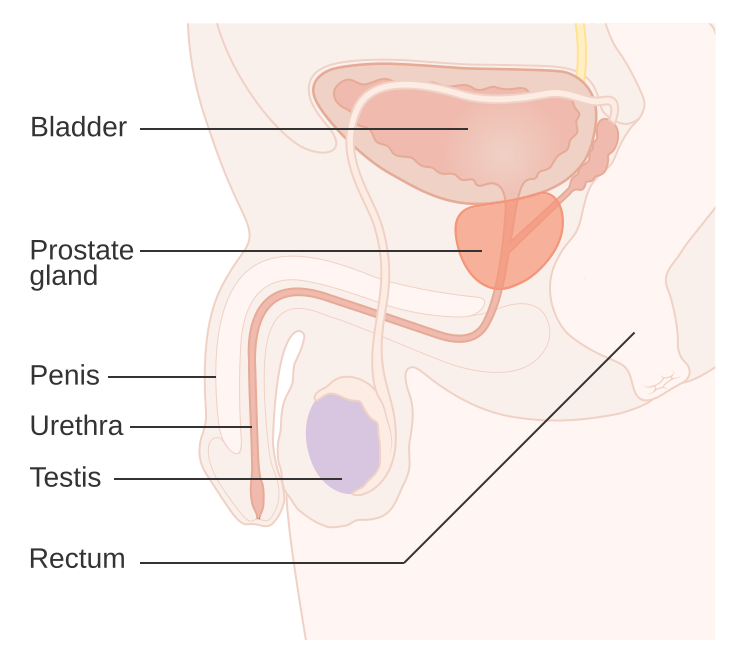
\includegraphics[width=0.7\textwidth]{background/Diagram_showing_the_position_of_the_prostate_and_rectum_CRUK_358.svg.png}
\caption{Visualization showing where a prostate is located\cite{prostate-rectum-image}.}
\end{figure}

\newpage
\subsection{Prostate cancer}
Prostate cancer is a tumour that grows in the prostate. During growth, it can press against the urethra, triggering the symptoms described below.
Cancer can spread to other organs of the body, so it is important to detect the disease early and monitor it properly. 
The 5-year survival rate for one with the condition is between 30-99 percent.

This cancer ranks as the world's second most common cancer among men, after lung cancer. In 2020, there were approximately 1.4 million diagnosed cases and 375,000 deaths worldwide\cite{culp_recent_2020}.
In Europe, it is the most commonly diagnosed cancer in males and the third leading cause of cancer-related deaths, what can be observed in Poland (Fig. [\ref{fig:prostate-cancer-occurences}]). 

\begin{figure}[H]
\begin{subfigure}[b]{0.5\textwidth}
    \centering
    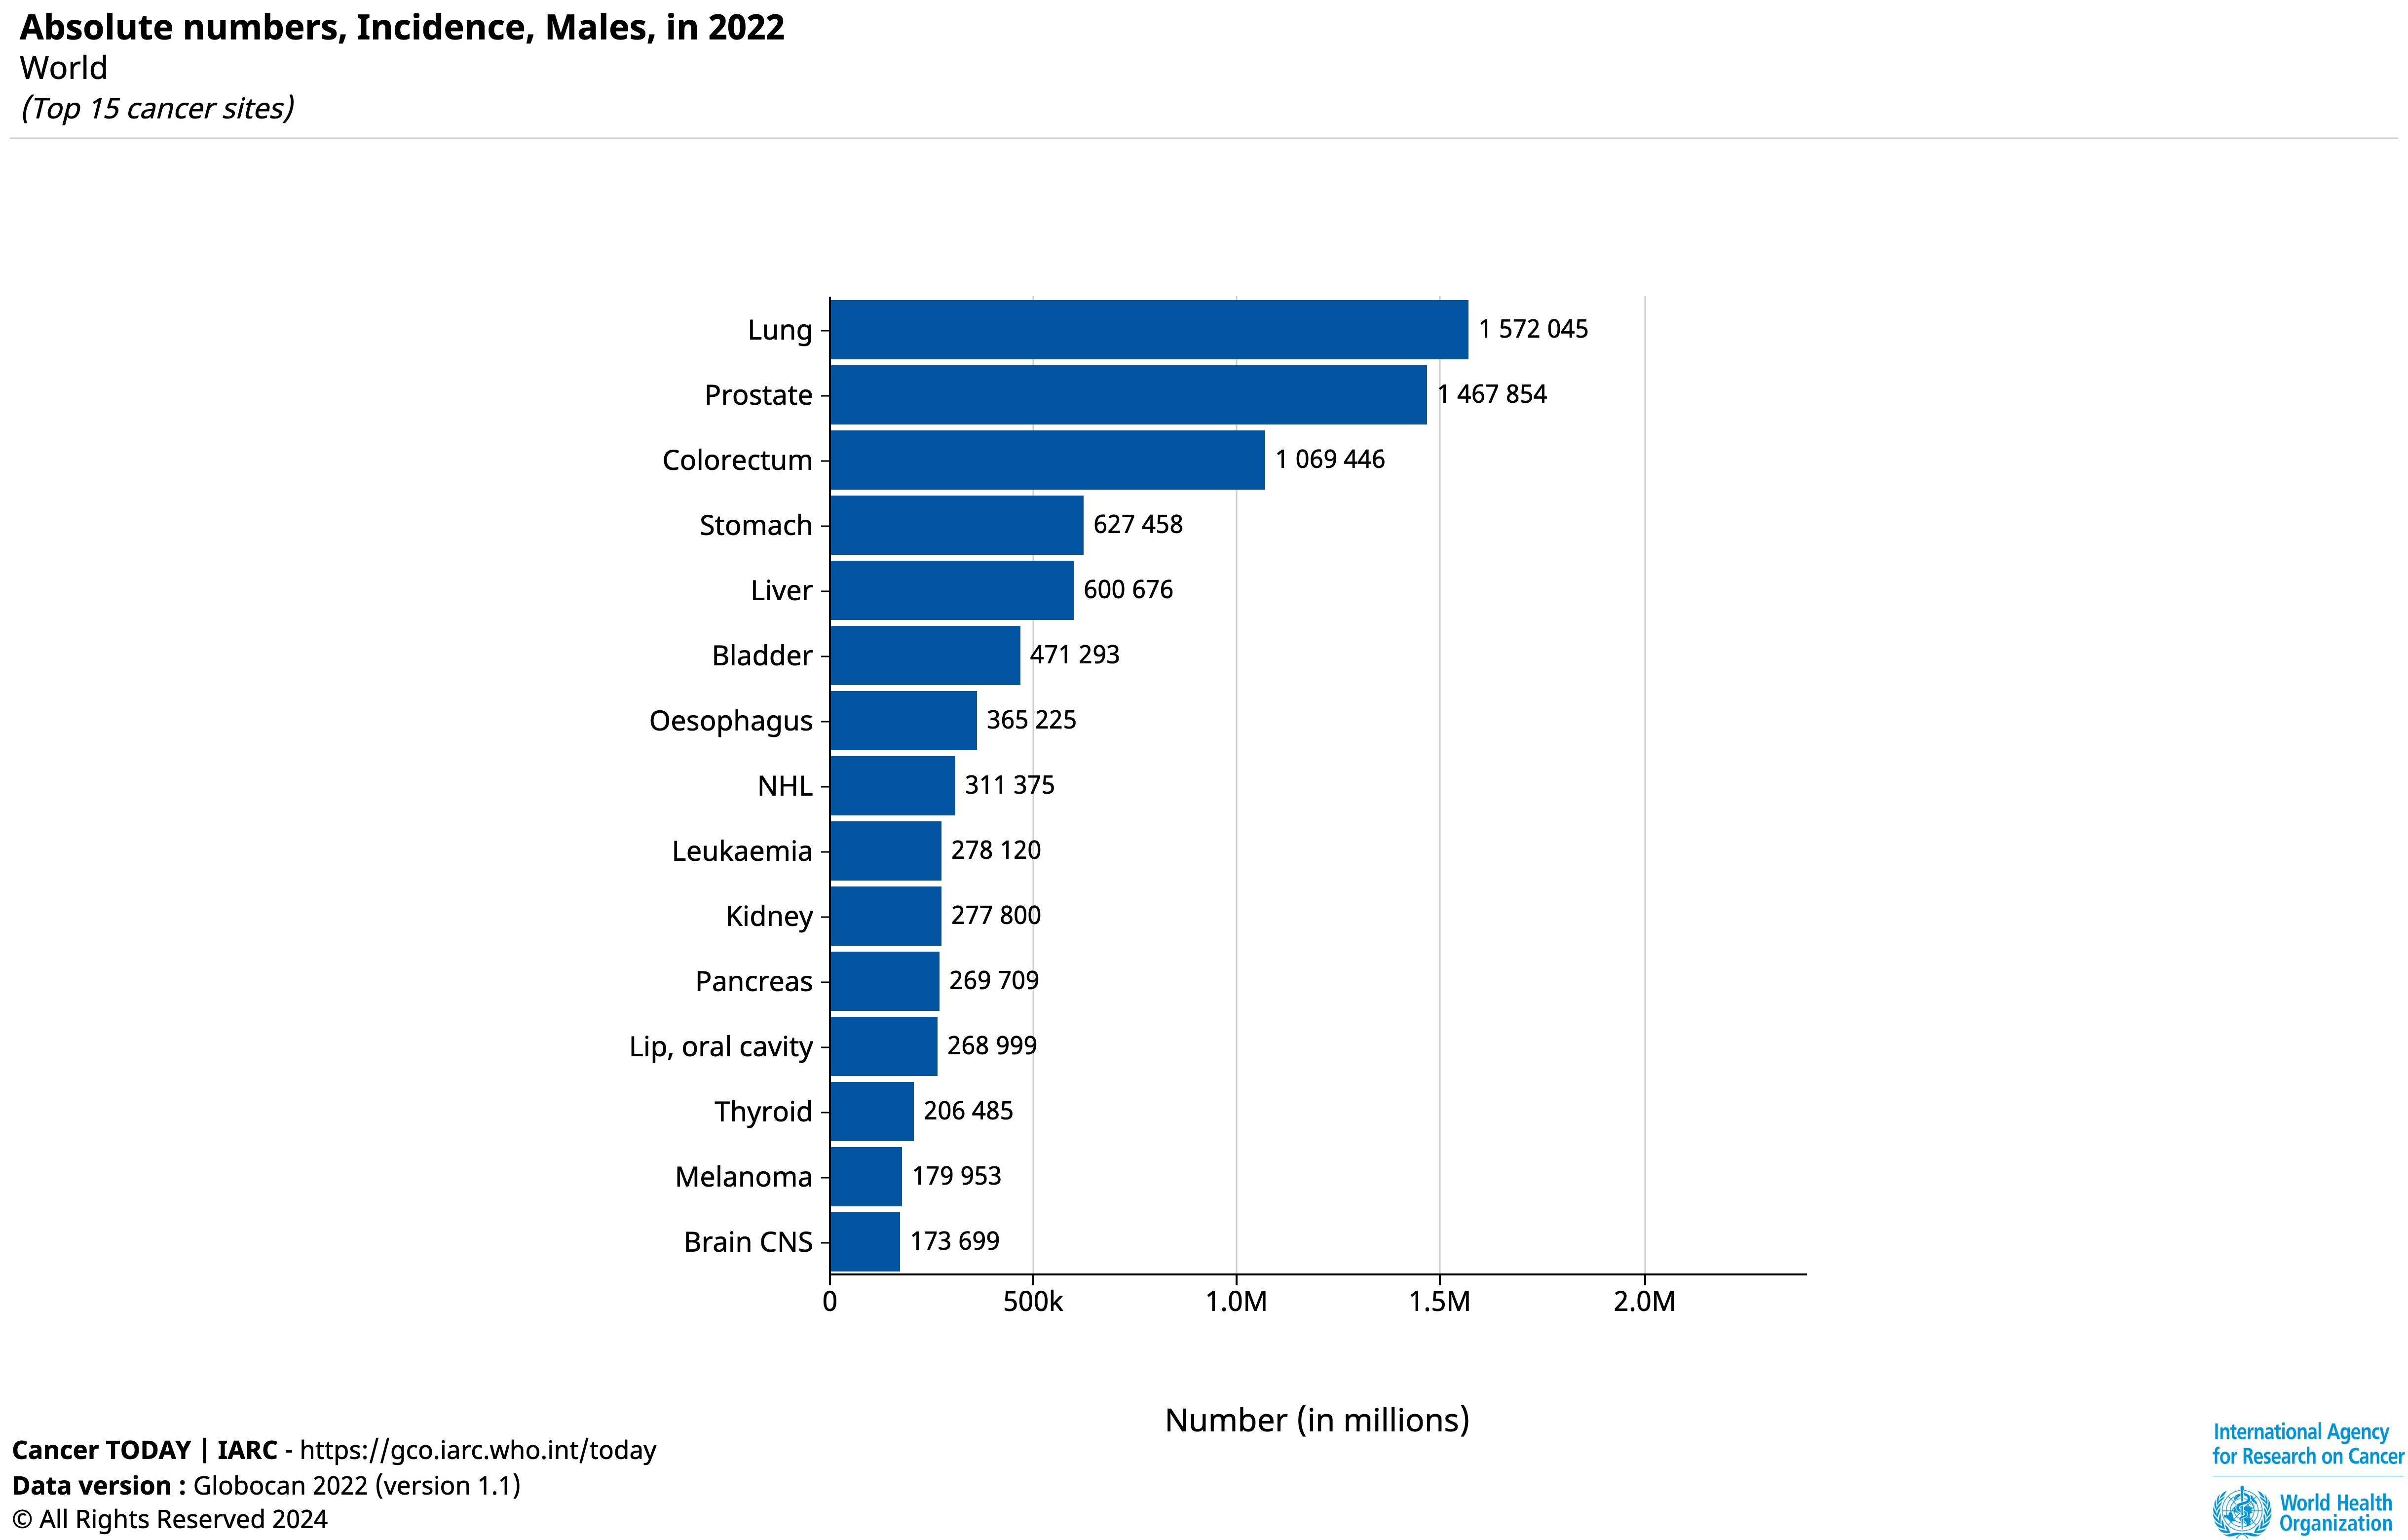
\includegraphics[width=1\linewidth]{background/graphic-absolute-numbers-inc-males-in-2022-world.png}
    \label{fig:pc-incidence-world}
\end{subfigure}
\begin{subfigure}[b]{0.5\textwidth}
    \centering
    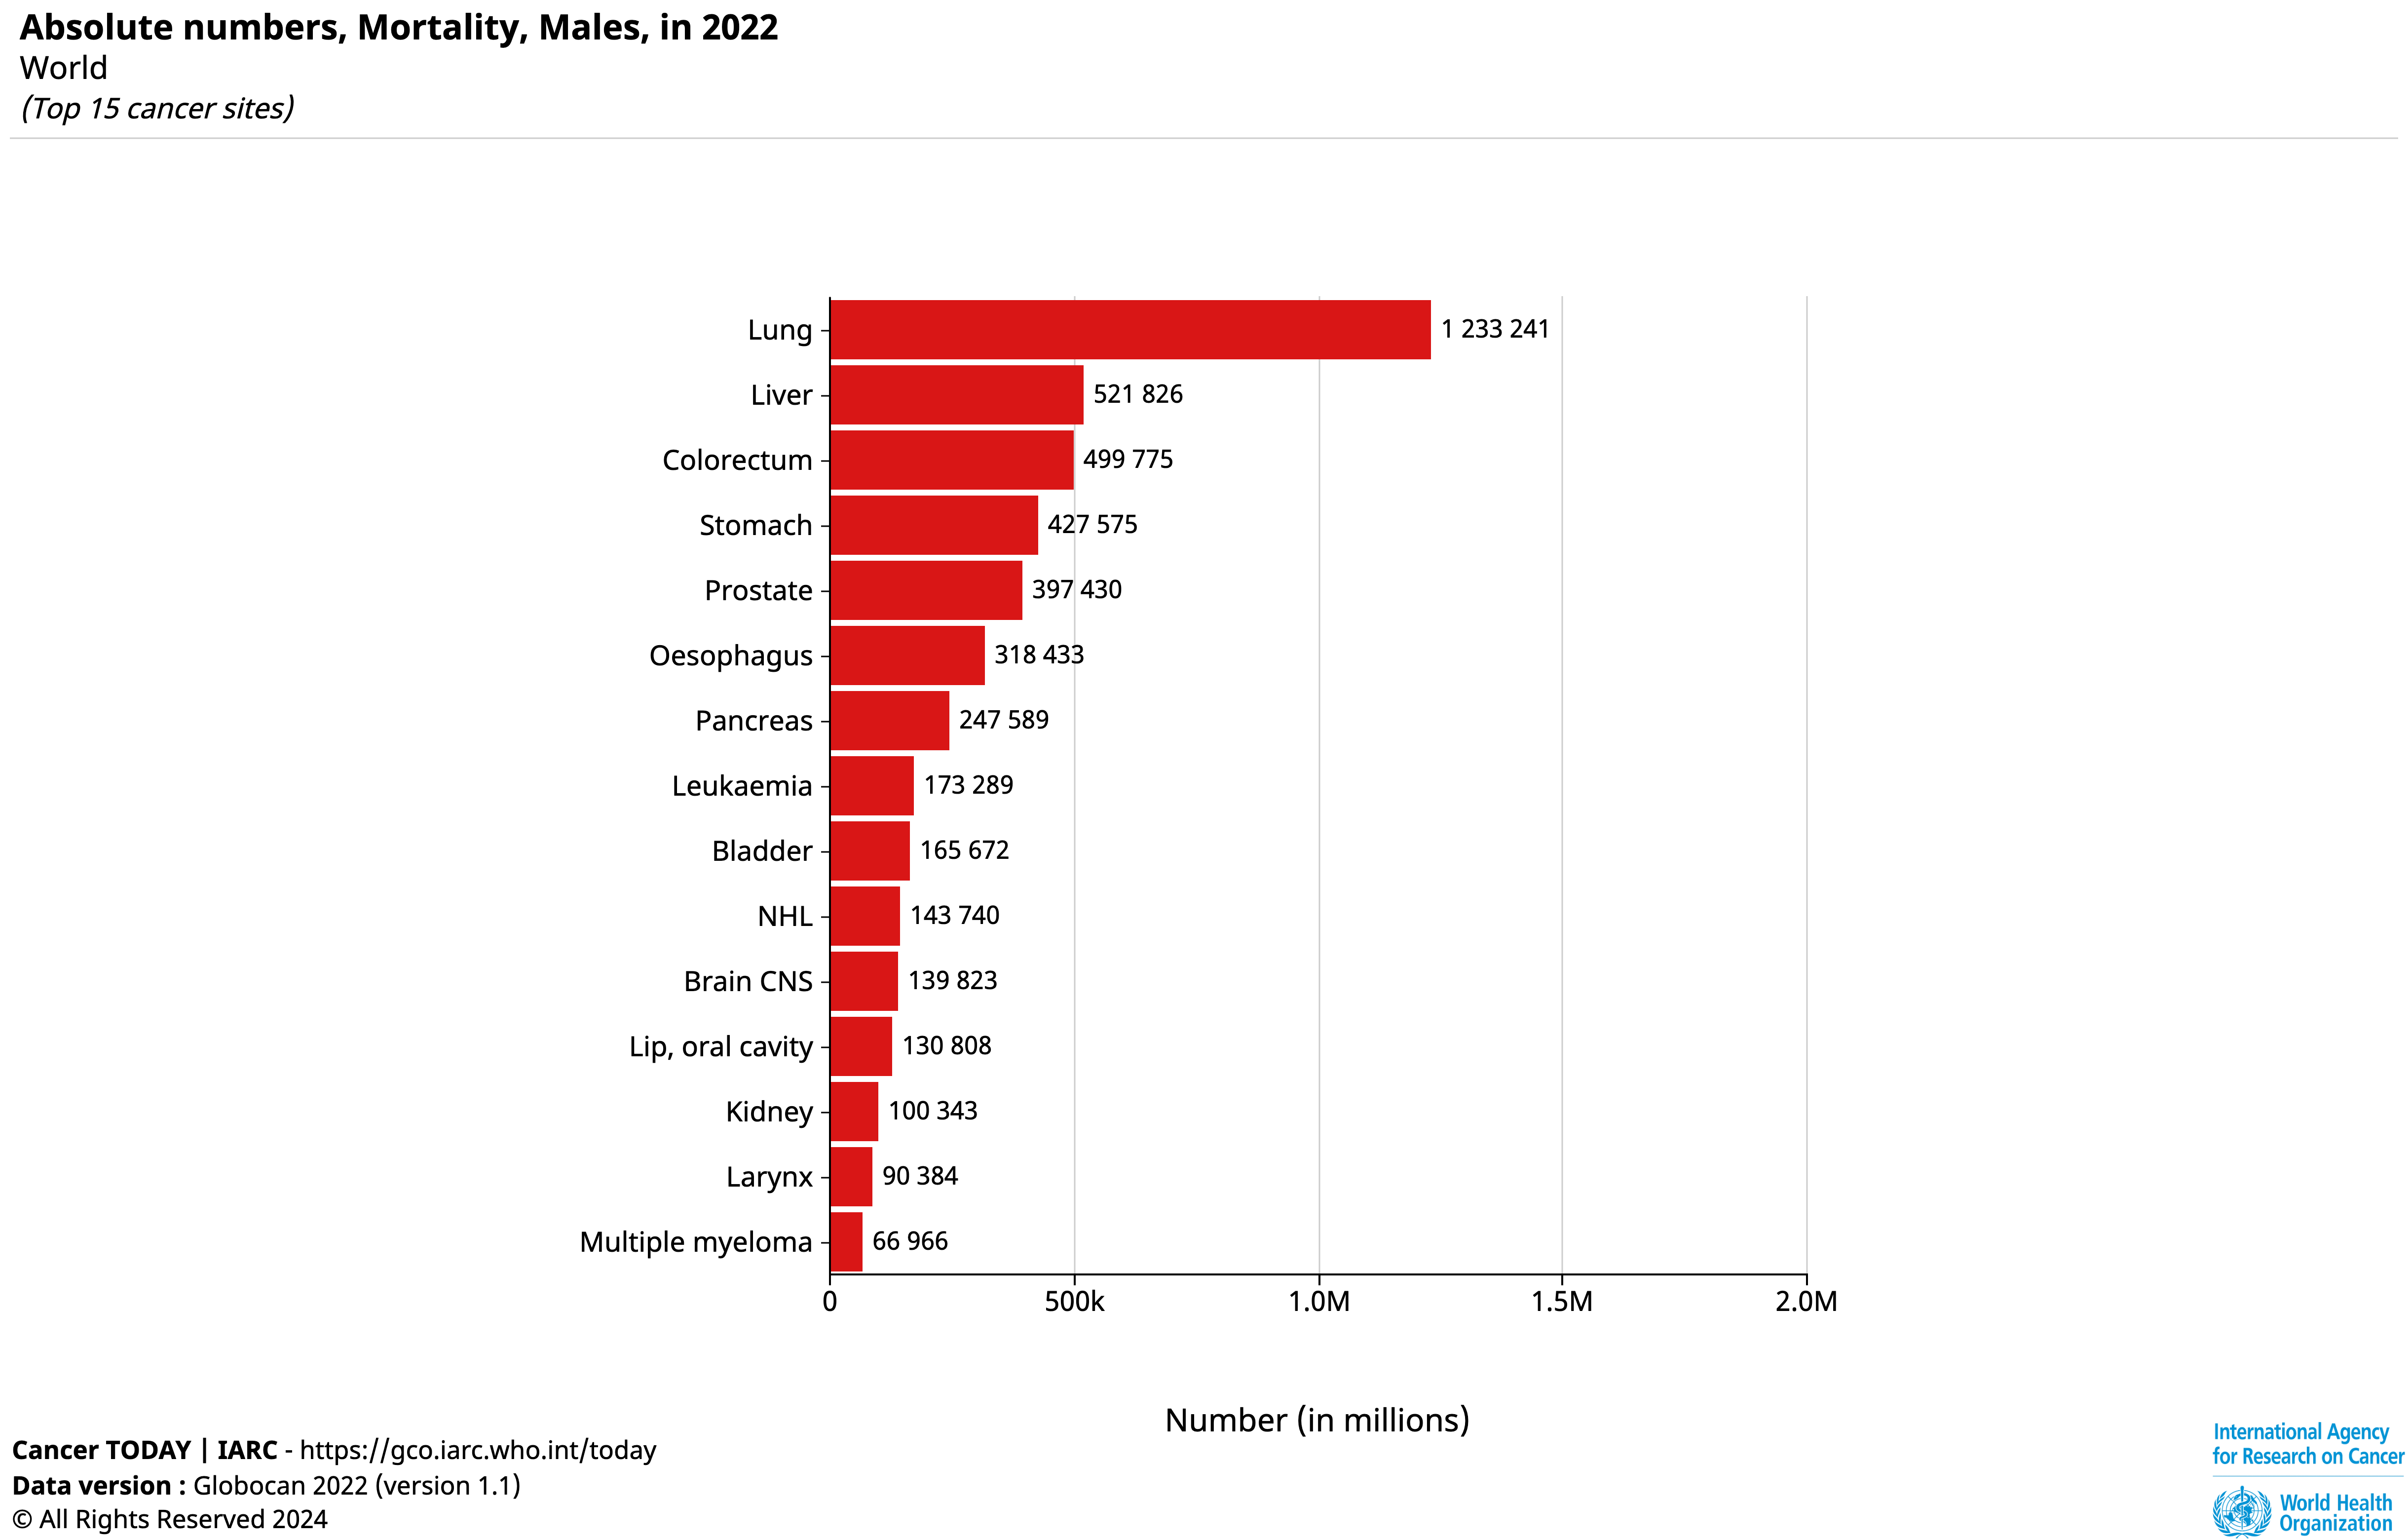
\includegraphics[width=1\linewidth]{background/graphic-absolute-numbers-mort-males-in-2022-world.png}
    \label{fig:pc-mortality-world}
\end{subfigure}
\caption{Absolute numbers of prostate cancer incidence and mortality in males in the world in 2022.\cite{gco_cancer_today}.}
\end{figure}

\begin{figure}[H]
    \centering
    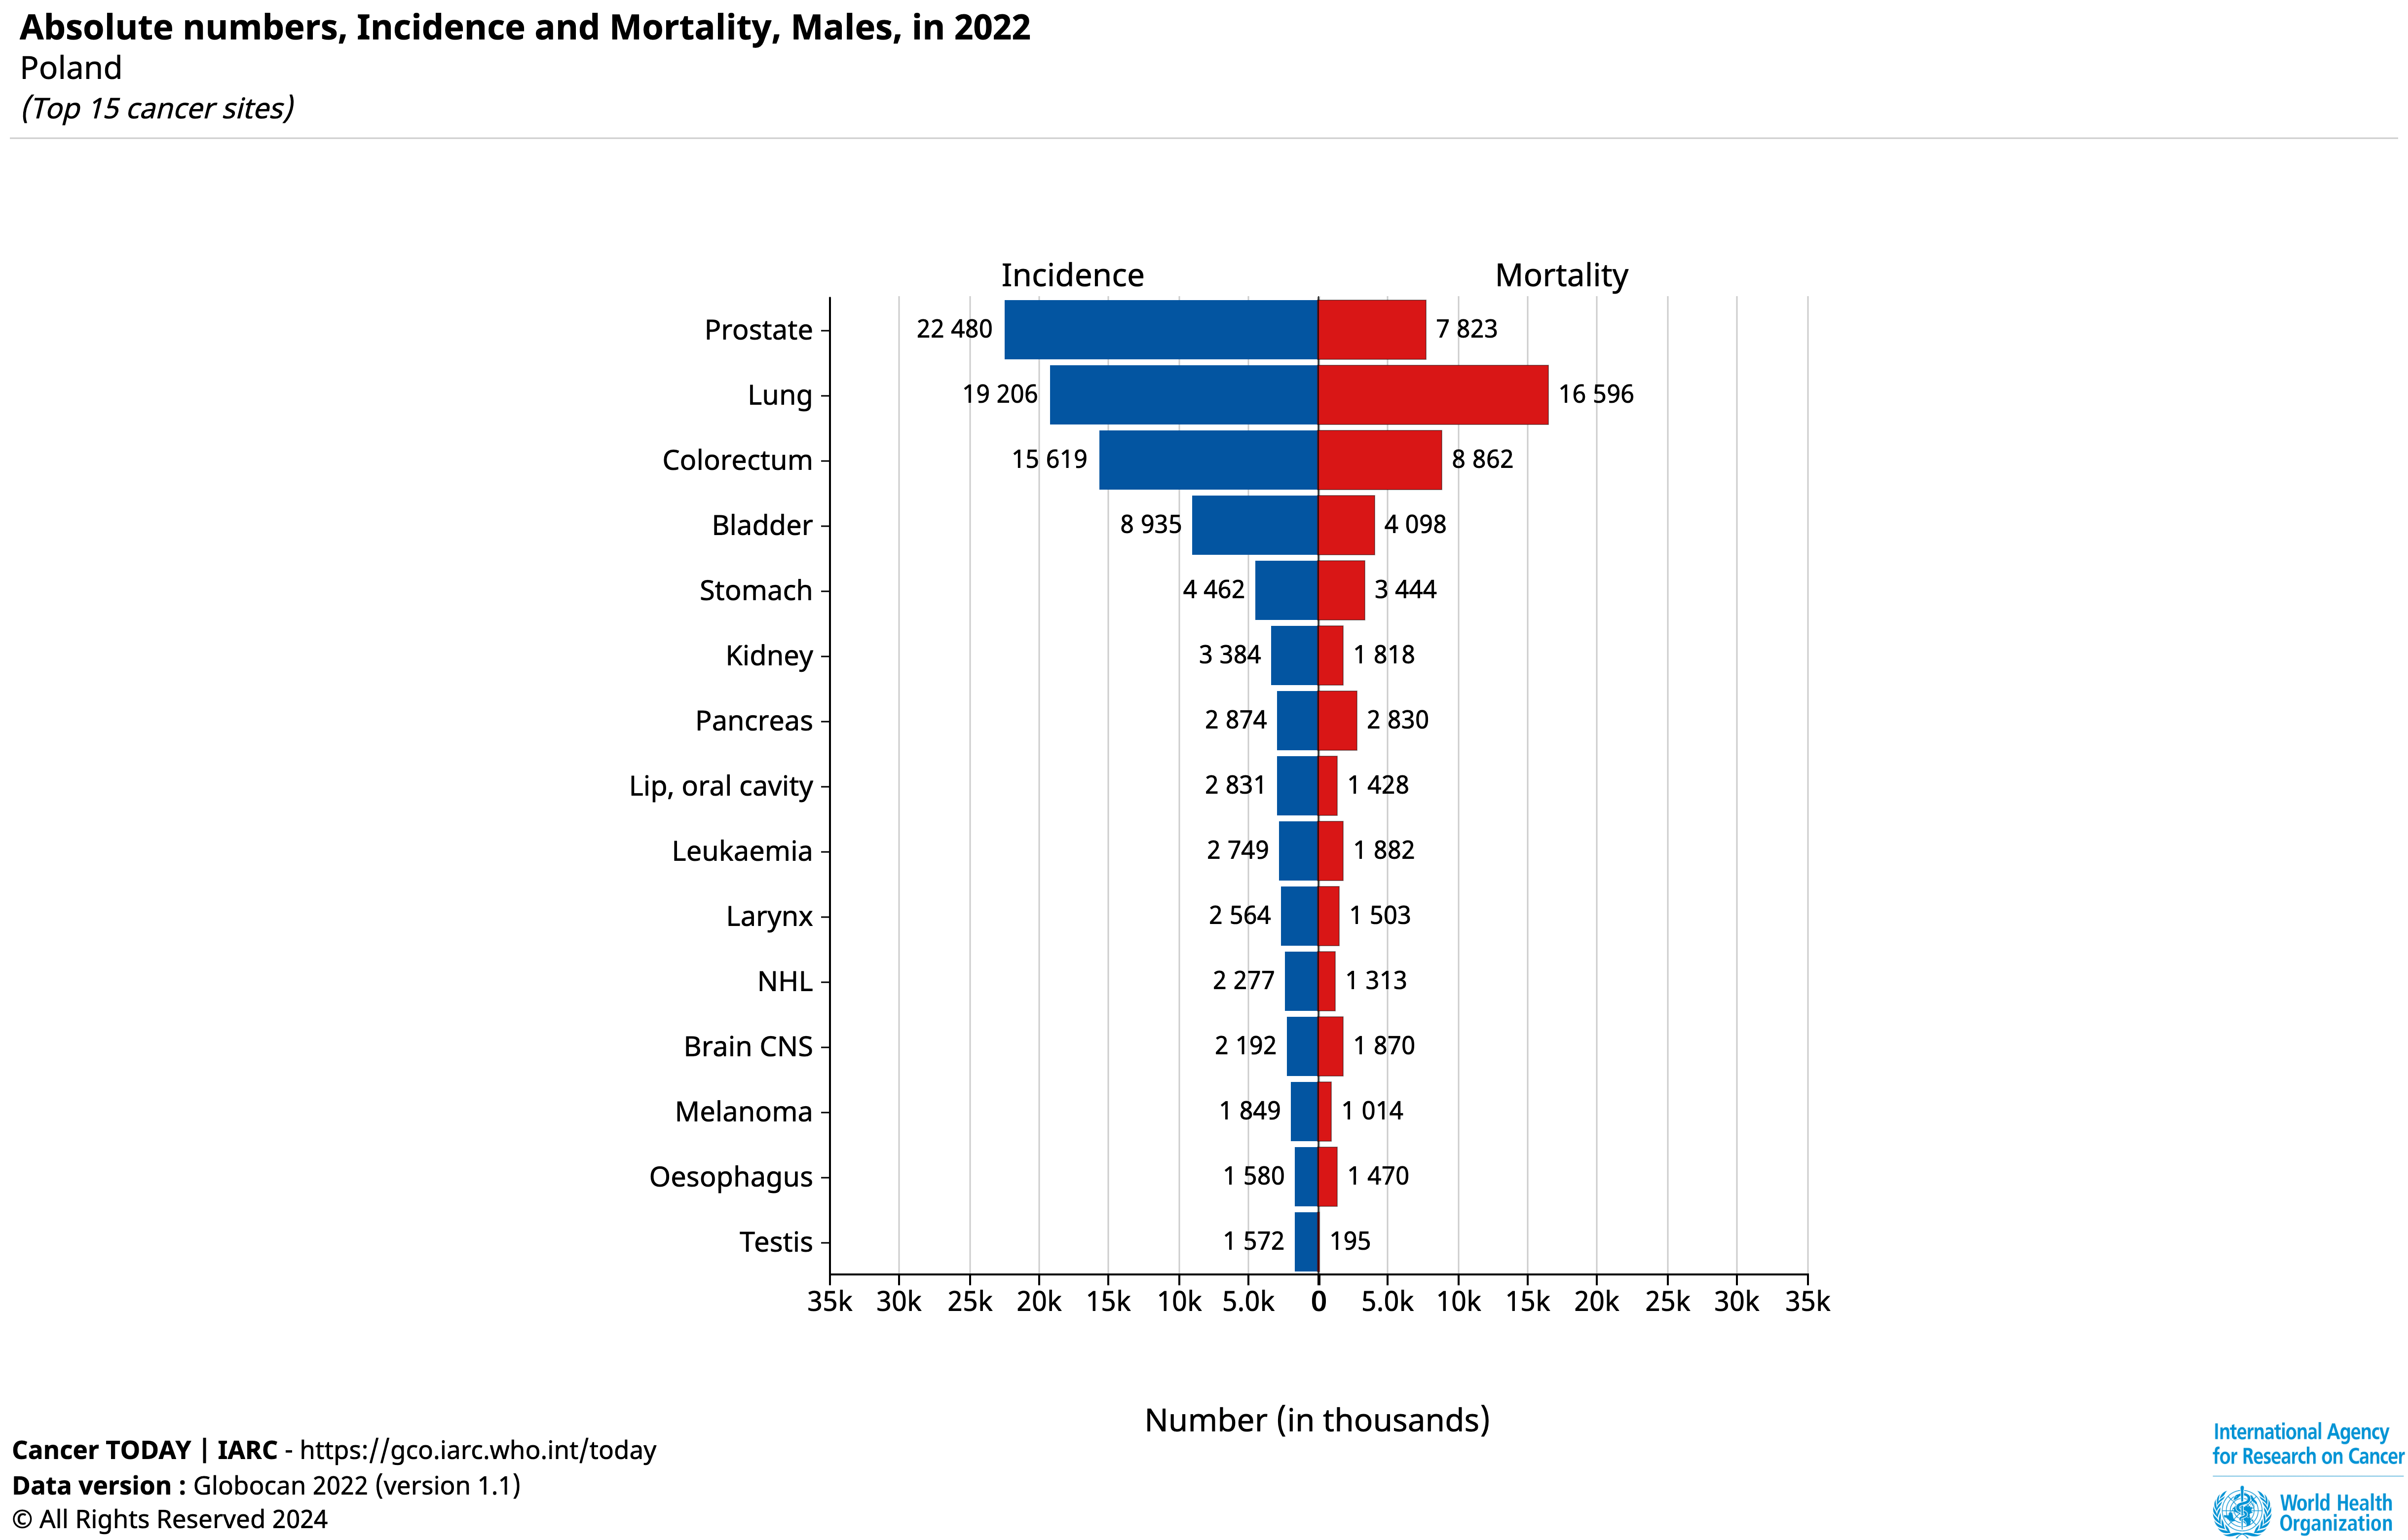
\includegraphics[width=0.5\linewidth]{background/graphic-absolute-numbers-inc-and-mort-males-in-2022-poland.png}
    \caption{Absolute numbers of prostate cancer incidence and mortality in males in Poland in 2022\cite{gco_cancer_today}}.
    \label{fig:prostate-cancer-occurences}
\end{figure}

Chris Parker, Prostate cancer specialist at the Institute of Cancer Research in the United Kingdom, says that even 80 percent of old men have prostate cancer, but they are never diagnosed with it\cite{nhs_choices_2024}. 


\begin{figure}[H]
    \centering
    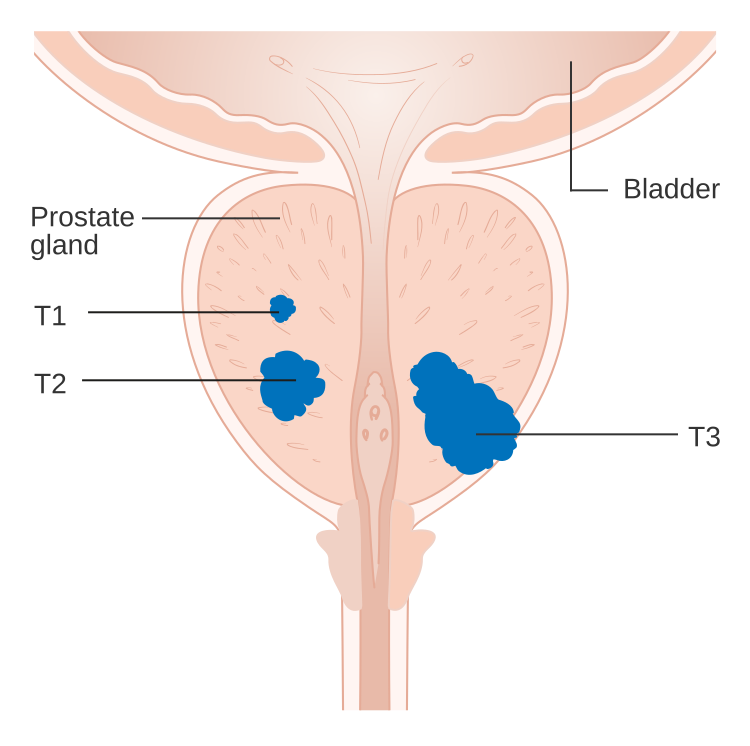
\includegraphics[width=0.5\linewidth]{background/Diagram_showing_T1-3_stages_of_prostate_cancer_CRUK_278.svg.png}
    \caption{Three stages of prostate cancer\cite{pc-stages}.}
    \label{fig:prostate-cancer-stages}
\end{figure}

\paragraph{Symptomps}\mbox{} \\

Prostate cancer can lead to\cite{prostate-cancer-symptomsandcauses_2024}\cite{nhs_choices_2024}:
\begin{itemize}
    \item troubles with urinating,
    \item blood in the urine,
    \item blood in the semen,
    \item bone pain,
    \item weight loose,
    \item erectile dysfunction,
    \item need to use toilet more frequently,
    \item need to use toilet more urgently.
\end{itemize}

\paragraph{Causes\cite{nhs_choices_2024}}\mbox{} \\
\indent Causes of prostate cancer of prostate cancer are not known. However, there are certain things that increase the risk of having the condition. 
Most cases of prostate cancer are diagnosed in men aged 50 or older. 
Men whose relatives were affected by the condition have a slightly increased risk of having it. Recent research suggests that obesity could have an influence on the risk of prostate cancer.

\paragraph{Diagnosis\cite{nhs_choices_2024}}\mbox{} \\
There are multiple tests that can help detect prostate cancer. 
Most commonly used tests are\cite{nhs_choices_2024}:
\begin{itemize}
    \item blood tests - Prostate-specific antigen (PSA) test, it measures the level of PSA in the blod; the test can help detect cancer in an early stage.
    \item physical examination,
    \item biopsy,
    \item medical imaging - MRI and CT scans.
\end{itemize}

\paragraph{Treating prostate cancer\cite{nhs_choices_2024}}
\begin{itemize}
    \item active surveillance,
    \item surigical removal of the prostate,
    \item radiation therapy,
    \item hormone therapy,
    \item chemotherapy.
    
\end{itemize}

% \newpage
\subsection{Medical imaging}
Medical imaging is the technique and process used to produce visual representations of the interior of a body for clinical evaluation and medical treatment. It enables doctors to examine the structures of the body, diagnose illnesses, direct treatments and track the progress of diseases. Various methods of medical imaging exist, each crafted to emphasize different aspects of the body's health. The main ones are the following.

\begin{itemize}
    \item Computed Tomography (CT),
    \item Magnetic Resonance Imaging (MRI),
    \item Ultrasound (USG),
    \item Positron Emission Tomography (PET).
\end{itemize}

\begin{figure}[H]
    \centering
    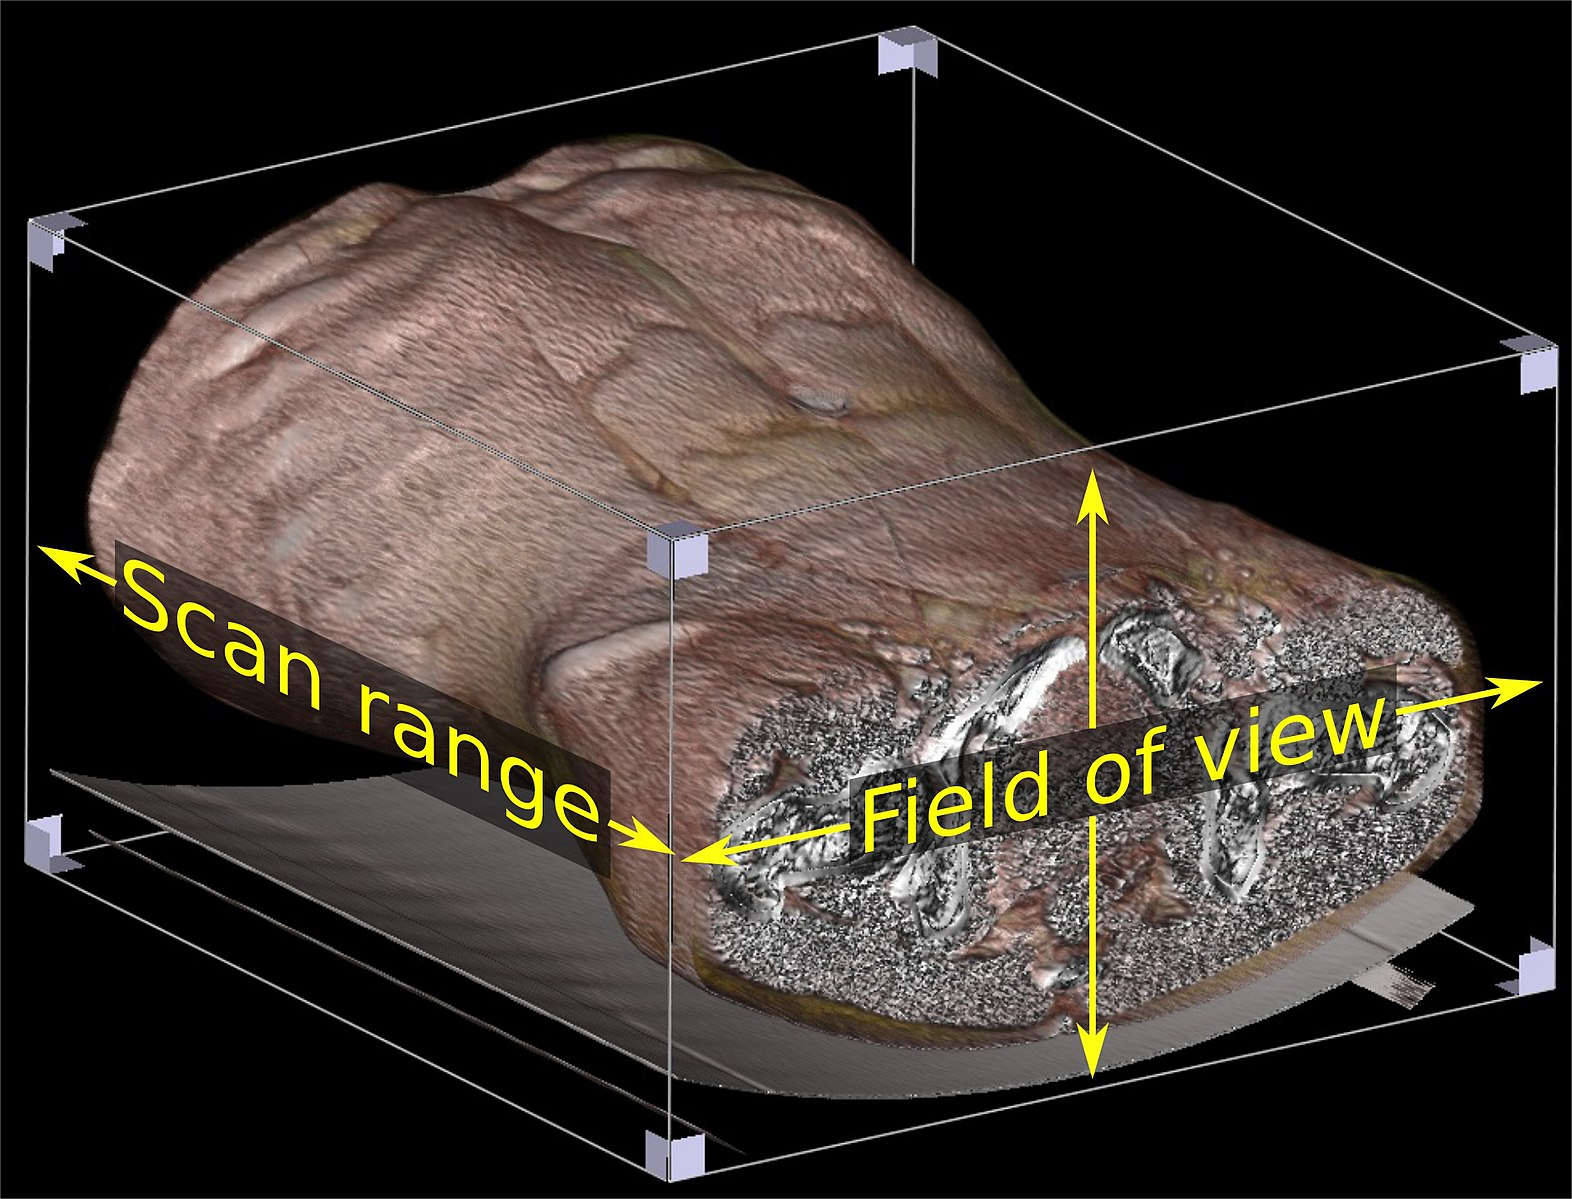
\includegraphics[width=0.5\linewidth]{background/1572px-Abdominal_CT_with_scan_range_and_field_of_view,_with_box_and_text.jpg}
    \caption{Abdominal CT scan\cite{abdominal-ct-scan}.}
    \label{fig:ct-scan-abdominal}
\end{figure}

In this study, our emphasis will be on computed tomography, as the dataset we are using was generated through this method. However, datasets acquired through other approaches could be similarly expanded using the deep learning techniques described later.

% \subsubsection{MRI- Magnetic resonance imaging}

% \begin{figure}[H]
%     \centering
%     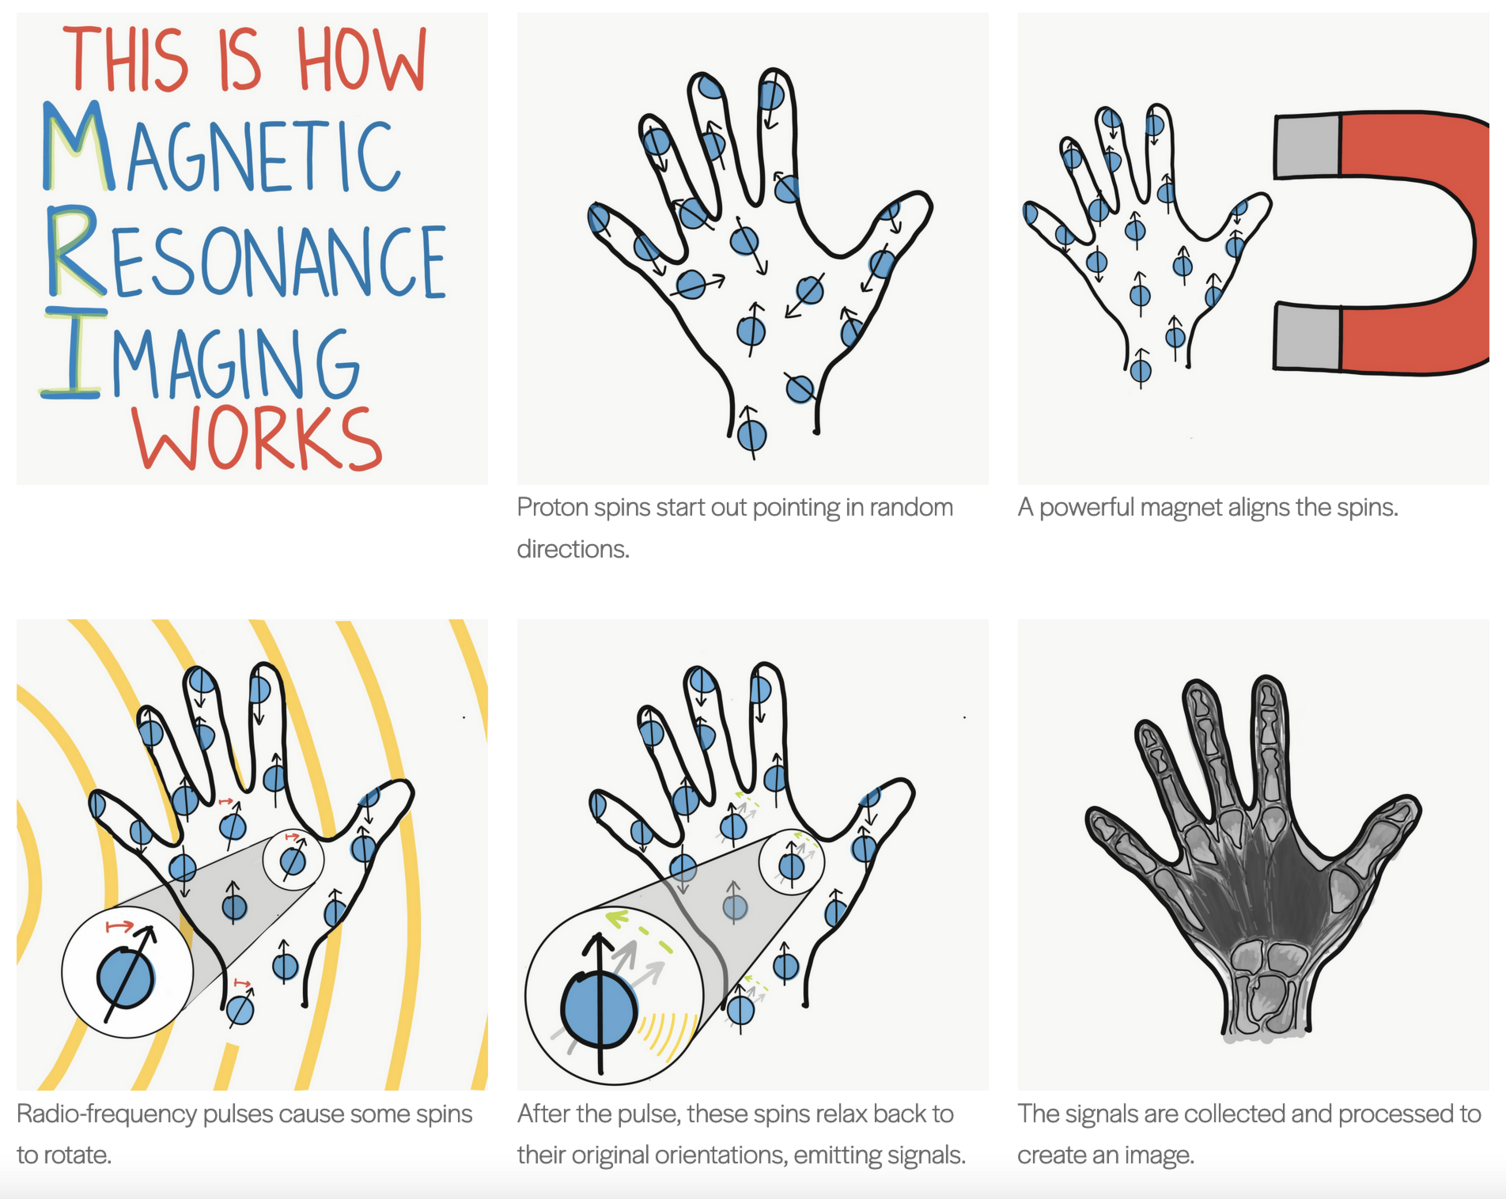
\includegraphics[width=0.99\linewidth]{background/Magnetic_Resonance_Imaging.png}
%     \caption{Explanation how magnetic resonance imaging (MRI) works\cite{mri-scan-how-it-works}.}
%     \label{fig:enter-label}
% \end{figure}

\newpage
\subsubsection{CT - Computed Tompography}
Computed tomography (CT) is a medical imaging technique that produces detailed cross-sectional images of the body. The word "tomography" comes from Ancient Greek, where "tomos" means "to slice" and "graphō" means "to write". 

The slicing of the human body is achieved using X-rays and advanced computer algorithms. Unlike conventional X-rays, which produce flat, two-dimensional images, CT scans produce 3D images by combining multiple X-ray measurements taken from different angles around the body. 

During a CT scan, an X-ray source rotates around the patient. Meanwhile, detectors on the opposite side capture the X-rays as they pass through the body. The X-rays are weakened as they pass through different tissues, such as bone, muscle and fat, which absorb different amounts of radiation. This rotating X-ray system produces multiple images or 'slices' of the body, typically only a few millimetres thick. A computer then processes these images to produce detailed cross-sectional images of the inside of the body. These multiple slices can be combined to create a 3D representation of the area being examined. 

% \begin{figure}[H]
%     \centering
%     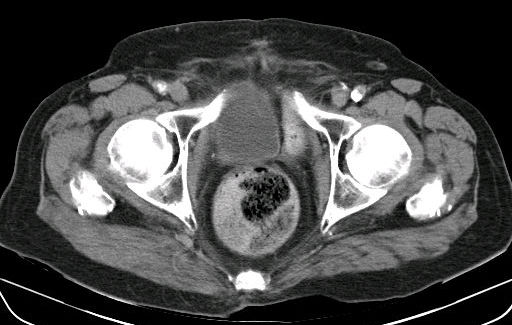
\includegraphics[width=0.5\linewidth]{background/ImpacFecal_149.jpg}
%     \caption{One slice of a tompography scan of prostate and pelvis\cite{ct-scan-prostate}.}
%     \label{fig:enter-label}
% \end{figure}
% - DICOM format for saving CT data.

\begin{figure}[H]
    \centering
    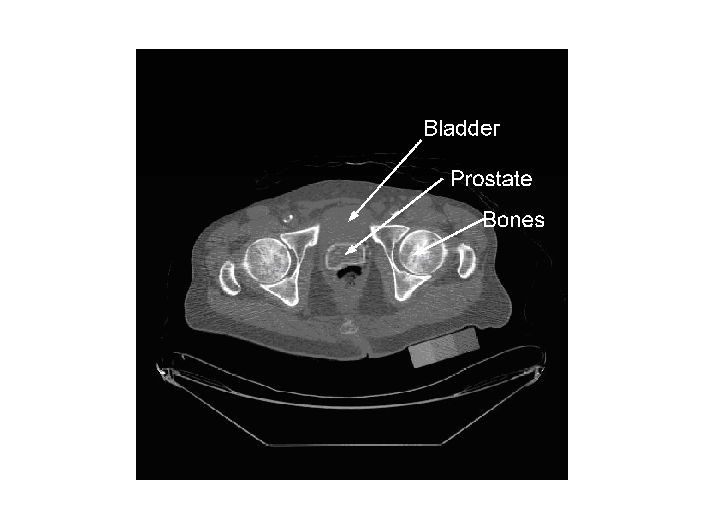
\includegraphics[width=0.9\linewidth]{background/A-typical-2-D-pelvic-CT-scan-Left-Manually-segmented-prostate-region-marked-by-a.png}
    \caption{Single layer from a 3-D pelvic CT scan. Segmented manually and marked by a radiologist\cite{inproceedings}.}
    \label{fig:enter-label}
\end{figure}

\newpage
\subsection{Cancer detection}
% Prostae cancer is usually detected using blood tests. Medicians do not use CT scans to diagnose the condition. They are used to check whether prostate cancer has spread to other parts of the body. 
Prostate cancer is detected by a combination of diagnostic tests, starting with a PSA (prostate specific antigen) blood test and a digital rectal examination. If abnormalities are found, a biopsy is often carried out to confirm the presence of cancer cells. Once diagnosed, imaging tests such as CT (computed tomography) scans are essential for staging the cancer, especially in advanced stages. CT scans can show whether the cancer has spread to other areas, such as lymph nodes, bones or distant organs. This information is crucial in determining the most effective treatment approach, including surgery, radiotherapy or systemic therapies.
\paragraph{Cancer detection using Artificial Intelligence}\mbox{}\\
\indent In the case of prostate cancer, AI is primarily used for segmentation rather than initial detection. Detection is typically done by other diagnostic means. Once prostate cancer is identified, AI plays a crucial role in analyzing medical imaging data, particularly CT scans. AI-powered segmentation algorithms, for example U-Nets, can precisely mark the boundaries of the prostate gland, tumor, and surrounding tissues in these scans. This accurate segmentation is essential for treatment planning. Determining the exact location and extent of a tumour can be the basis for targeted radiotherapy or surgery. AI can also help monitor treatment. It can aid track the cancer progress and detect subtle changes in tumour size or shape over time. While AI improves the accuracy and efficiency of image analysis, it is important to note that it is a tool to assist healthcare professionals rather than a stand-alone diagnostic method. 

\paragraph{Limitations}\mbox{}\\
\indent One of the limitations of using AI in this context is the need for large and diverse datasets to train such models. Unfortunately, the medical imaging field suffers from training data insufficiency caused by data privacy, lack of standardized ways of collecting such data by multiple institutions, and throughput of CT scanners. 
This problem raised the idea of using data augmentation techniques in order to enlarge already existing datasets and it formed the basis for the subject of this thesis.
% \paragraph{State of the art techniques for cancer detection}

\newpage
\subsection{Data augmentation}
Data augmentation is a technique for enlarging existing dataset with new samples created from already existing ones. There exist many techniques that allow us to do so. The more traditional ones focus on transformations of the original images. However, with the rise of artificial intelligence, generative techniques have emerged that allow us to generate artificial samples using deep learning models. In this work, we will focus on generative models that can create synthetic samples from Gaussian noise. 

% \begin{figure}[H]
%     \centering
%     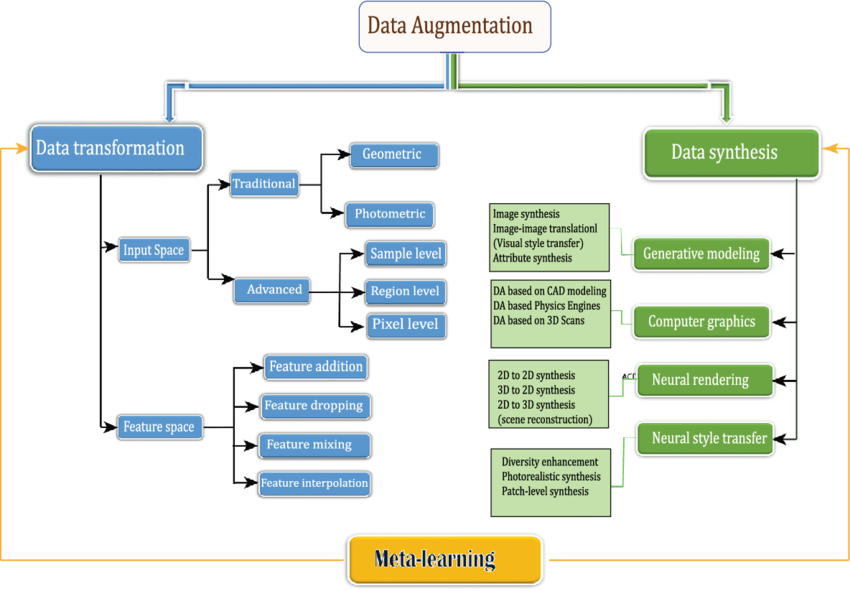
\includegraphics[width=0.99\linewidth]{background/Taxonomy-of-data-augmentation-approaches-used-in-this-survey.png}
%     \caption{Data augmentation taxonomy\cite{Mumuni2022-ka}.}
%     \label{fig:enter-label}
% \end{figure}

\begin{figure}[H]
    \centering
    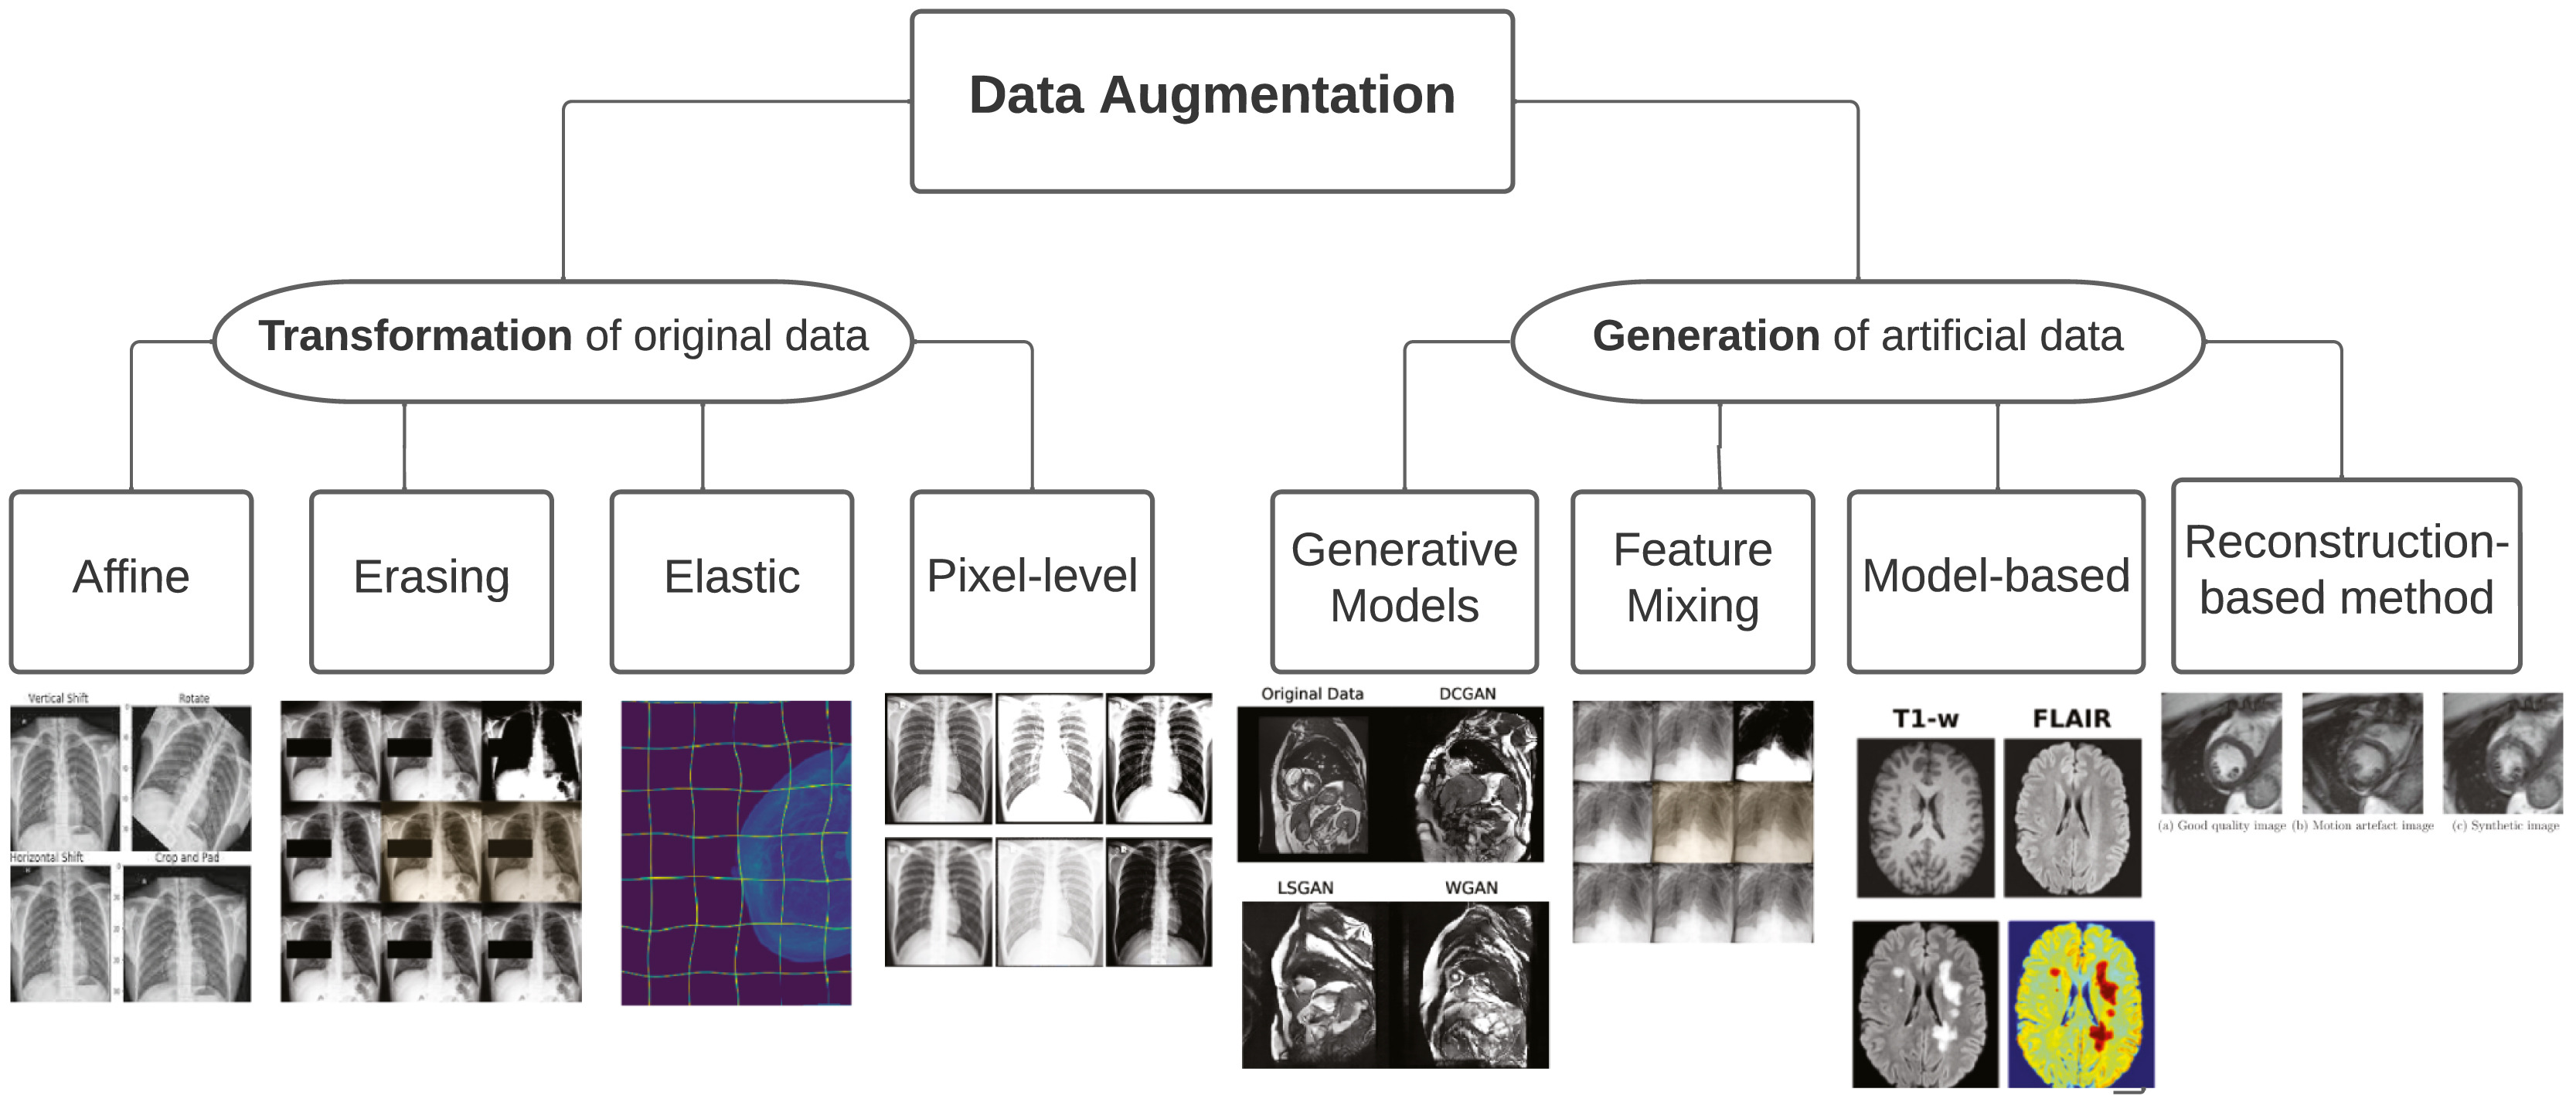
\includegraphics[width=0.99\linewidth]{background/taxonomy-data-augmentation.jpg}
    \caption{Data augmentation taxonomy\cite{GARCEA2023106391}.}
    \label{fig:enter-label}
\end{figure}

% The types of transformations
% \paragraph{Affine transformations} are geometric transformations that preserve lines and parallelism. They do not preserve angles and distances. Exemplary are: rotating, translating, scaling, horizontal and vertical shifting, cropping, padding, shearing.

% \paragraph{Erasing transformation} are used to replace some part of an image with some fixed value or random noise. 

% \paragraph{Pixel level}



\subsection{Generative Medical Imaging}
Medical imaging field in the AI landscape suffers from insufficient data. Thus scientists around the world started to explore generative networks. Now they are the most popular solution for the generation of medical images\cite{osuala2023data}.
Generative models provide a greater potential for data augmentation, in comparison to transformation techniques, by producing a wider variety of samples. However, these methods are much more complex and require significant computational resources.

Artificial samples obtained this way may not have the same visual characteristics or distribution as the original set. Additionally, the samples obtained in this way may include artifacts, even invisible to the human eye, that could be harmful to the models that would be trained on them.
\subsection{State of the art techniques for generative medical imaging}
\newpage
\section{Concept engineering}
\subsection{Possible data augmentation techniques}

\subsubsection{Core concepts}
\paragraph{CNN - Convolutional Neural Network}\mbox{}\\

Convolutional neural networks are used to extract intermediate representations of the input. They take advantage of convolutional filters with weights that are learned during training. Such convolutional filters create a convolutional layer. An image passed through a first convolutional layer creates the feature maps. Convolutional layers can be stacked together, creating in the result a convolutional network.
Convolutional layers are usually combined with subsampling techniques, such as pooling. 

\begin{figure}[H]
    \centering
    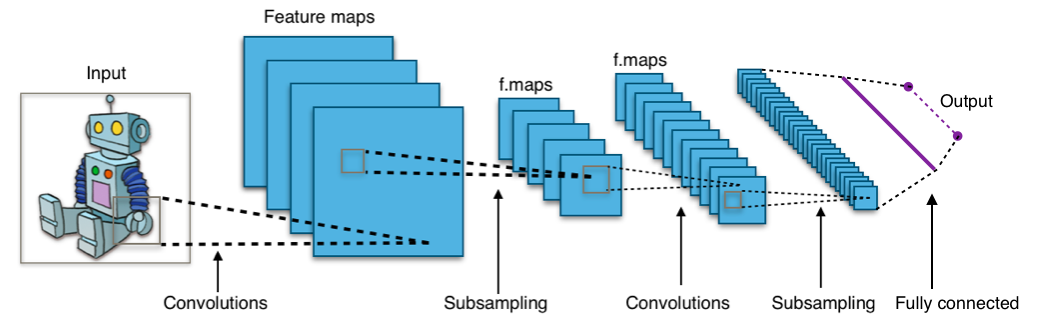
\includegraphics[width=\linewidth]{concept_engineering/Typical_cnn.png}
    \caption{Typical architecture of a convolutional neural network\cite{cnn-typical}.}
    \label{fig:cnn}
\end{figure}


\paragraph{Autoencoder}\mbox{}\\
\begin{figure}[H]
    \centering
    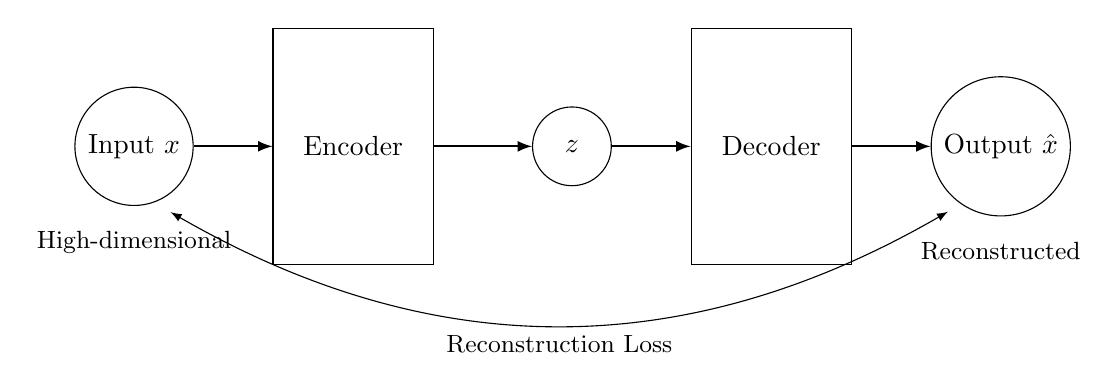
\begin{tikzpicture}[
    box/.style={draw, minimum width=2cm, minimum height=3cm, text width=1.8cm, align=center},
    smallbox/.style={draw, minimum width=1.5cm, minimum height=1.2cm, text width=1.3cm, align=center},
    arrow/.style={->, >=latex, thick},
    label/.style={font=\small}
]

% Components
\node[circle, draw] (input) {Input $x$};
\node[box, right=1cm of input] (encoder) {Encoder};

% Latent space
\node[right=1cm of encoder] (latent) {};
\node[circle, draw, minimum size=1cm, right=0cm of latent] (z) {$z$};

\node[box, right=1cm of z] (decoder) {Decoder};
\node[circle, draw, right=1cm of decoder] (output) {Output $\hat{x}$};

% Reparameterization trick

% Connections
\draw[arrow] (input) -- (encoder);
\draw[arrow] (encoder) -- (z);
\draw[arrow] (z) -- (decoder);
\draw[arrow] (decoder) -- (output);

% Labels
\node[label, below=0.2cm of input] {High-dimensional};
% \node[label, above=0.2cm of mu] {Latent space};
\node[label, below=0.2cm of output] {Reconstructed};

% KL Divergence

% Reconstruction Loss
\draw[<->, >=latex, bend right=30] ($(input.south west)+(1,-0.3)$) to node[below, font=\small] {Reconstruction Loss} ($(output.south east)+(-1.3,-0.2)$);
\end{tikzpicture}
    \caption{Visualization of an autoencoder. Circles are tensors, rectangles neural networks.}
    \label{fig:autoencoder}
\end{figure}
\indent Autoencoder is an architecture of deep learning model that consists of two deep neural networks - Encoder and Decoder. The task of the encoder is to transform the input into latent representation of the input. Usually it compresses it, for example to a vector or smaller matrix/tensor. Decoder then takes such latent representation and transforms it back to its original form. 

The loss function between input $x$ and output $\hat{x}$ is usually one of the following: L1, L2, MSE.

\paragraph{U-Net}\mbox{}\\
\indent U-Net is a special type of convolutional neural network, originally built for the task of image segmentation, especially in medical imaging. Its architecture resembles a U-shape, similar to an autoencoder. The encoder on the left side reduces the input image size while capturing significant features. The right side increases resolution and performs tasks like segmentation, utilizing the features extracted by the encoder via "skip connections." Despite the similarity, U-Net is not considered an autoencoder due to the use of skip connections.

\begin{figure}[H]
    \centering
    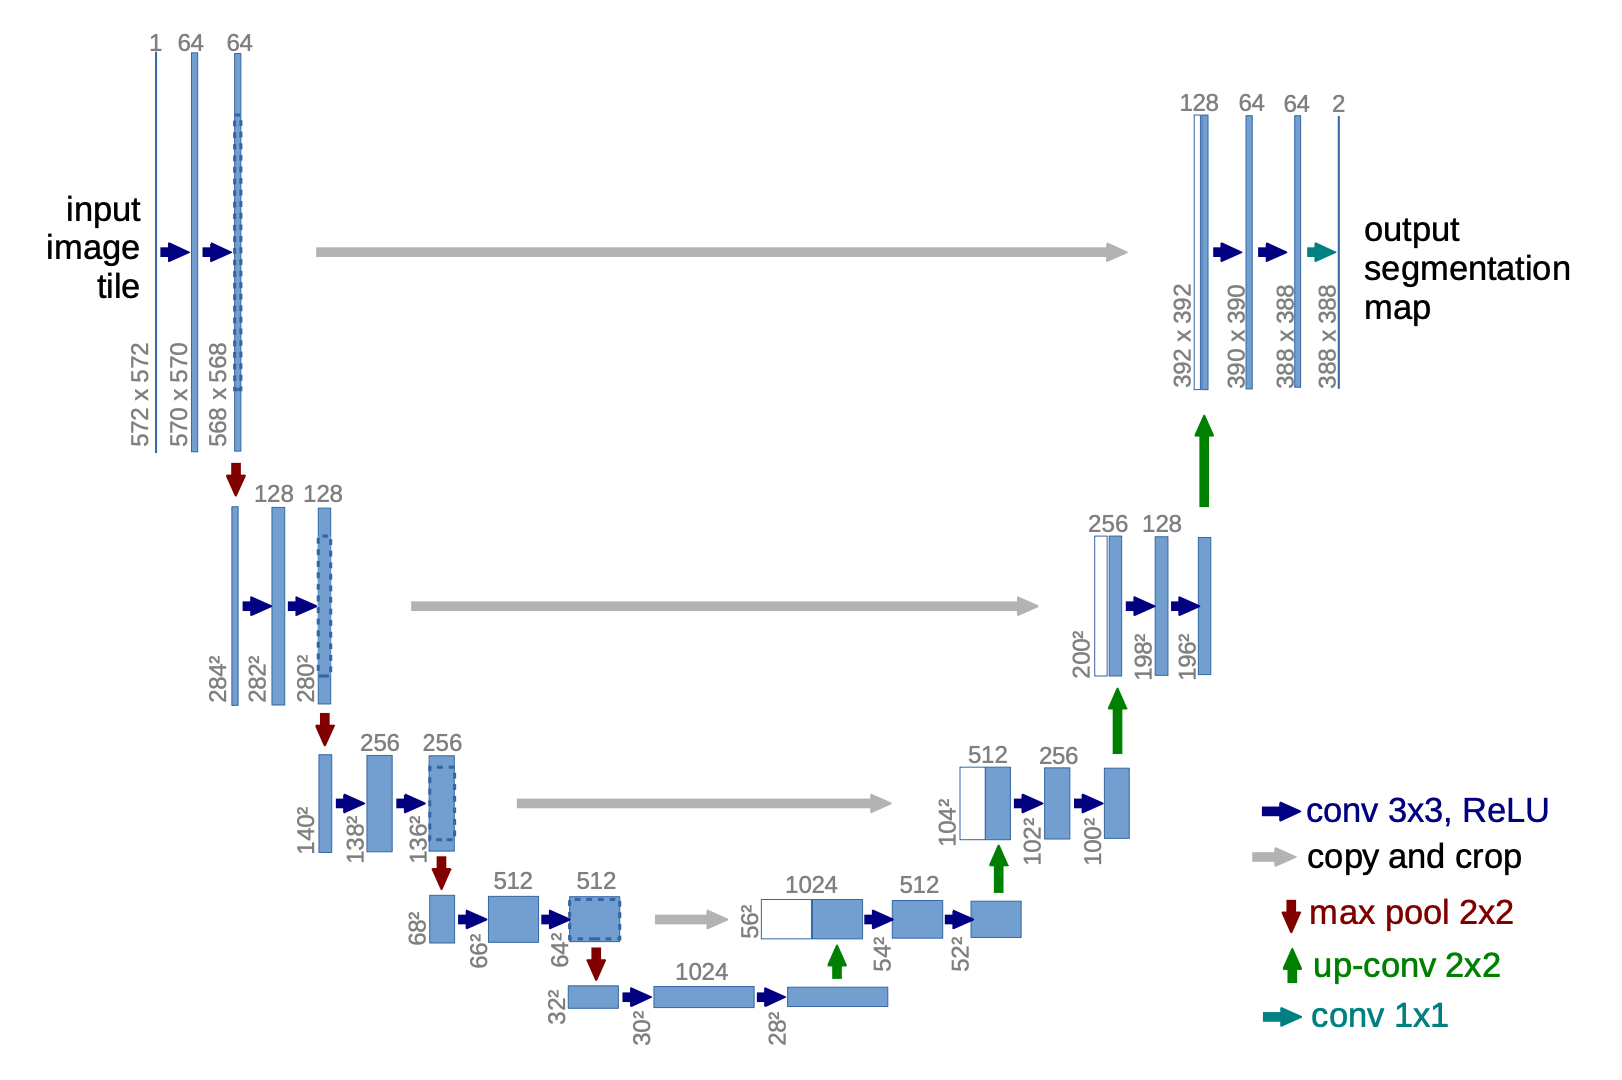
\includegraphics[width=0.9\linewidth]{concept_engineering/unet/U-net.png}
    \caption{U-Net architecture\cite{RFB15a}.}
    \label{fig:unet}
\end{figure}



\newpage
\subsubsection{GANS}

\begin{figure}[H]
    \centering
    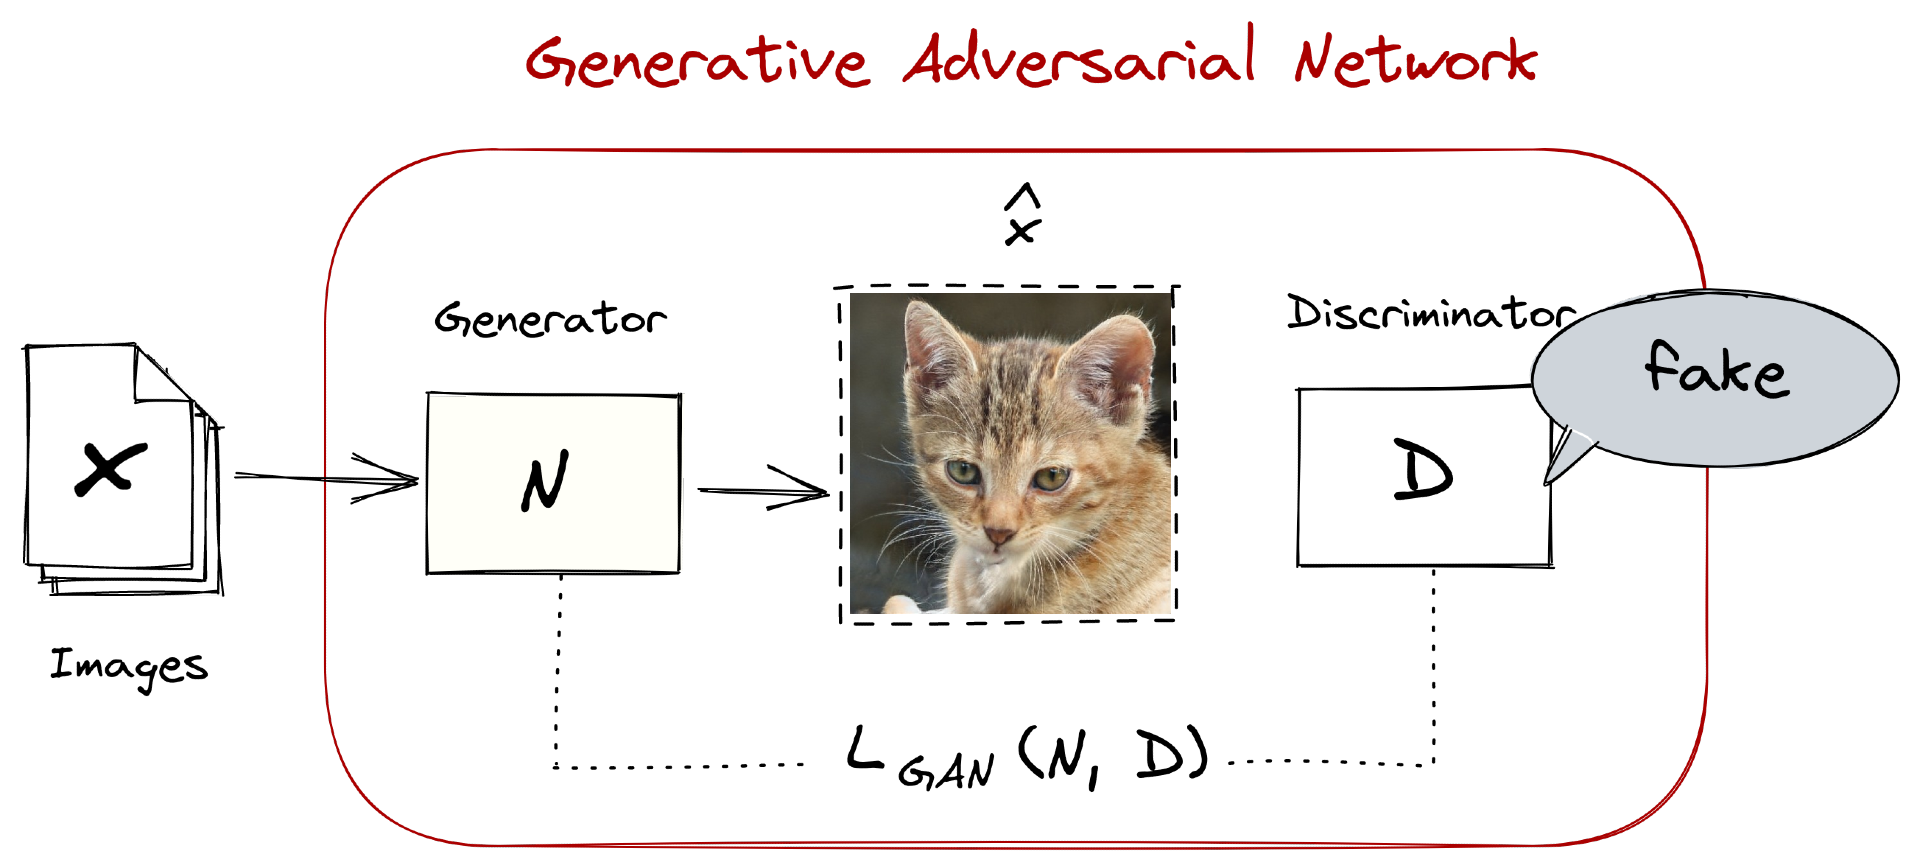
\includegraphics[width=0.9\linewidth]{concept_engineering/vqgan/vqgan_gan_inside.png}
    \caption{Caption}
    \label{fig:gan}
\end{figure}

Generative Adversarial Networks (GANs) are deep learning models that consist of two neural networks.
The first is a generator \( G \), which is responsible for generating false samples from random noise, and the second is a discriminator \( D \), which tries to detect which samples are false.
The generator and the discriminator compete in a minimax game. The two networks are trained simultaneously with opposite goals.

Mathematically, the goal of GANs is represented by the following minimax objective function:

\begin{equation}
\min_G \max_D V(D, G) = \mathbb{E}_{x \sim p_{data}(x)}[\log D(x)] + \mathbb{E}_{z \sim p_z(z)}[\log (1 - D(G(z)))]
\end{equation}
where:

\begin{itemize}
\item \( D(x) \) represents the probability that the discriminator correctly identifies a real sample \( x \),

\item \( G(z)=\hat{x} \) represents the synthetic data generated by the generator from random noise \( z \), in our case CT scan,

\item \( p_{data}(x) \) is the data distribution of the real samples,

\item \( p_z(z) \) is the distribution of the random noise input to the generator.
\end{itemize}

\paragraph{Loss function}\mbox{}\\
\indent GAN loss function can be calculated as
\begin{equation}
    L_{GAN}(N,D) = [\log D(x) + log(1-D(\hat{x}))]
\label{loss_gan}
\end{equation}
However it often leads to discriminator being too good on the beginning and in result generator stops training. To mitigate that, each neural network, generator and discriminator has their own loss.
The loss function of the discriminator is typically defined as

\begin{equation}
L_D = - \left( \mathbb{E}_{x \sim p_{data}(x)}[\log D(x)] + \mathbb{E}_{z \sim p_z(z)}[\log (1 - D(\hat{x}))] \right)
\end{equation}


This loss encourages the discriminator to maximize its ability to distinguish real from false data. On the other hand, the generator loss function can be defined as


\begin{equation}
L_G = - \mathbb{E}_{z \sim p_z(z)}[\log D(\hat{x})]
\end{equation}


This loss encourages the generator to improve the quality of the false samples by "fooling" the discriminator into classifying them as real. Training continues until the generator produces samples that are indistinguishable from the real data, at which point the discriminator cannot distinguish between real and generated samples and a Nash equilibrium\footnote{\url{https://en.wikipedia.org/wiki/Nash_equilibrium}} is reached.

GANs have had a significant impact in areas such as image generation, data augmentation and even super-resolution tasks, but their training can be unstable due to problems such as vanishing gradients. 


\paragraph{Generation of CT scan}\mbox{}\\

To generate an artifical CT scan using GAN, one should sample a Gaussian noise tensor $z$ from $\mathcal{N}(0,1)$, of shape the same as the generator input, and then pass it to a generator, which would produce a synthetic CT scan as a result.
\newpage
\subsubsection{Diffusion}
% \paragraph{Forward diffusion process}\mbox{} \\
% \begin{equation}
%     q(\mathbf{x}_{t}|\mathbf{x}_0)=\mathcal{N}(\mathbf{x}_{t};\sqrt{\bar{\alpha}_{t}}\mathbf{x}_0,(1-\bar{\alpha}_{t})\mathbf{I})
% \end{equation}

% \begin{equation}
% \mathbf{x}_{t}=\sqrt{\alpha_{t}}\mathbf{x}_{t-1}+\sqrt{1-\alpha_{t}}\boldsymbol{\epsilon},\quad\boldsymbol{\epsilon}\sim\mathcal{N}(0,\mathbf{I}).
% \end{equation}

% \begin{aligned}
% \mathbf{x}_t 
% &= \sqrt{\alpha_t}\mathbf{x}_{t-1} + \sqrt{1 - \alpha_t}\boldsymbol{\epsilon}_{t-1} & \text{ ;where } \boldsymbol{\epsilon}_{t-1}, \boldsymbol{\epsilon}_{t-2}, \dots \sim \mathcal{N}(\mathbf{0}, \mathbf{I}) \\
% &= \sqrt{\alpha_t \alpha_{t-1}} \mathbf{x}_{t-2} + \sqrt{1 - \alpha_t \alpha_{t-1}} \bar{\boldsymbol{\epsilon}}_{t-2} & \text{ ;where } \bar{\boldsymbol{\epsilon}}_{t-2} \text{ merges two Gaussians (*).} \\
% &= \dots \\
% &= \sqrt{\bar{\alpha}_t}\mathbf{x}_0 + \sqrt{1 - \bar{\alpha}_t}\boldsymbol{\epsilon} \\
% q(\mathbf{x}_t \vert \mathbf{x}_0) &= \mathcal{N}(\mathbf{x}_t; \sqrt{\bar{\alpha}_t} \mathbf{x}_0, (1 - \bar{\alpha}_t)\mathbf{I})
% \end{aligned}

\begin{figure}[h]
    \centering
    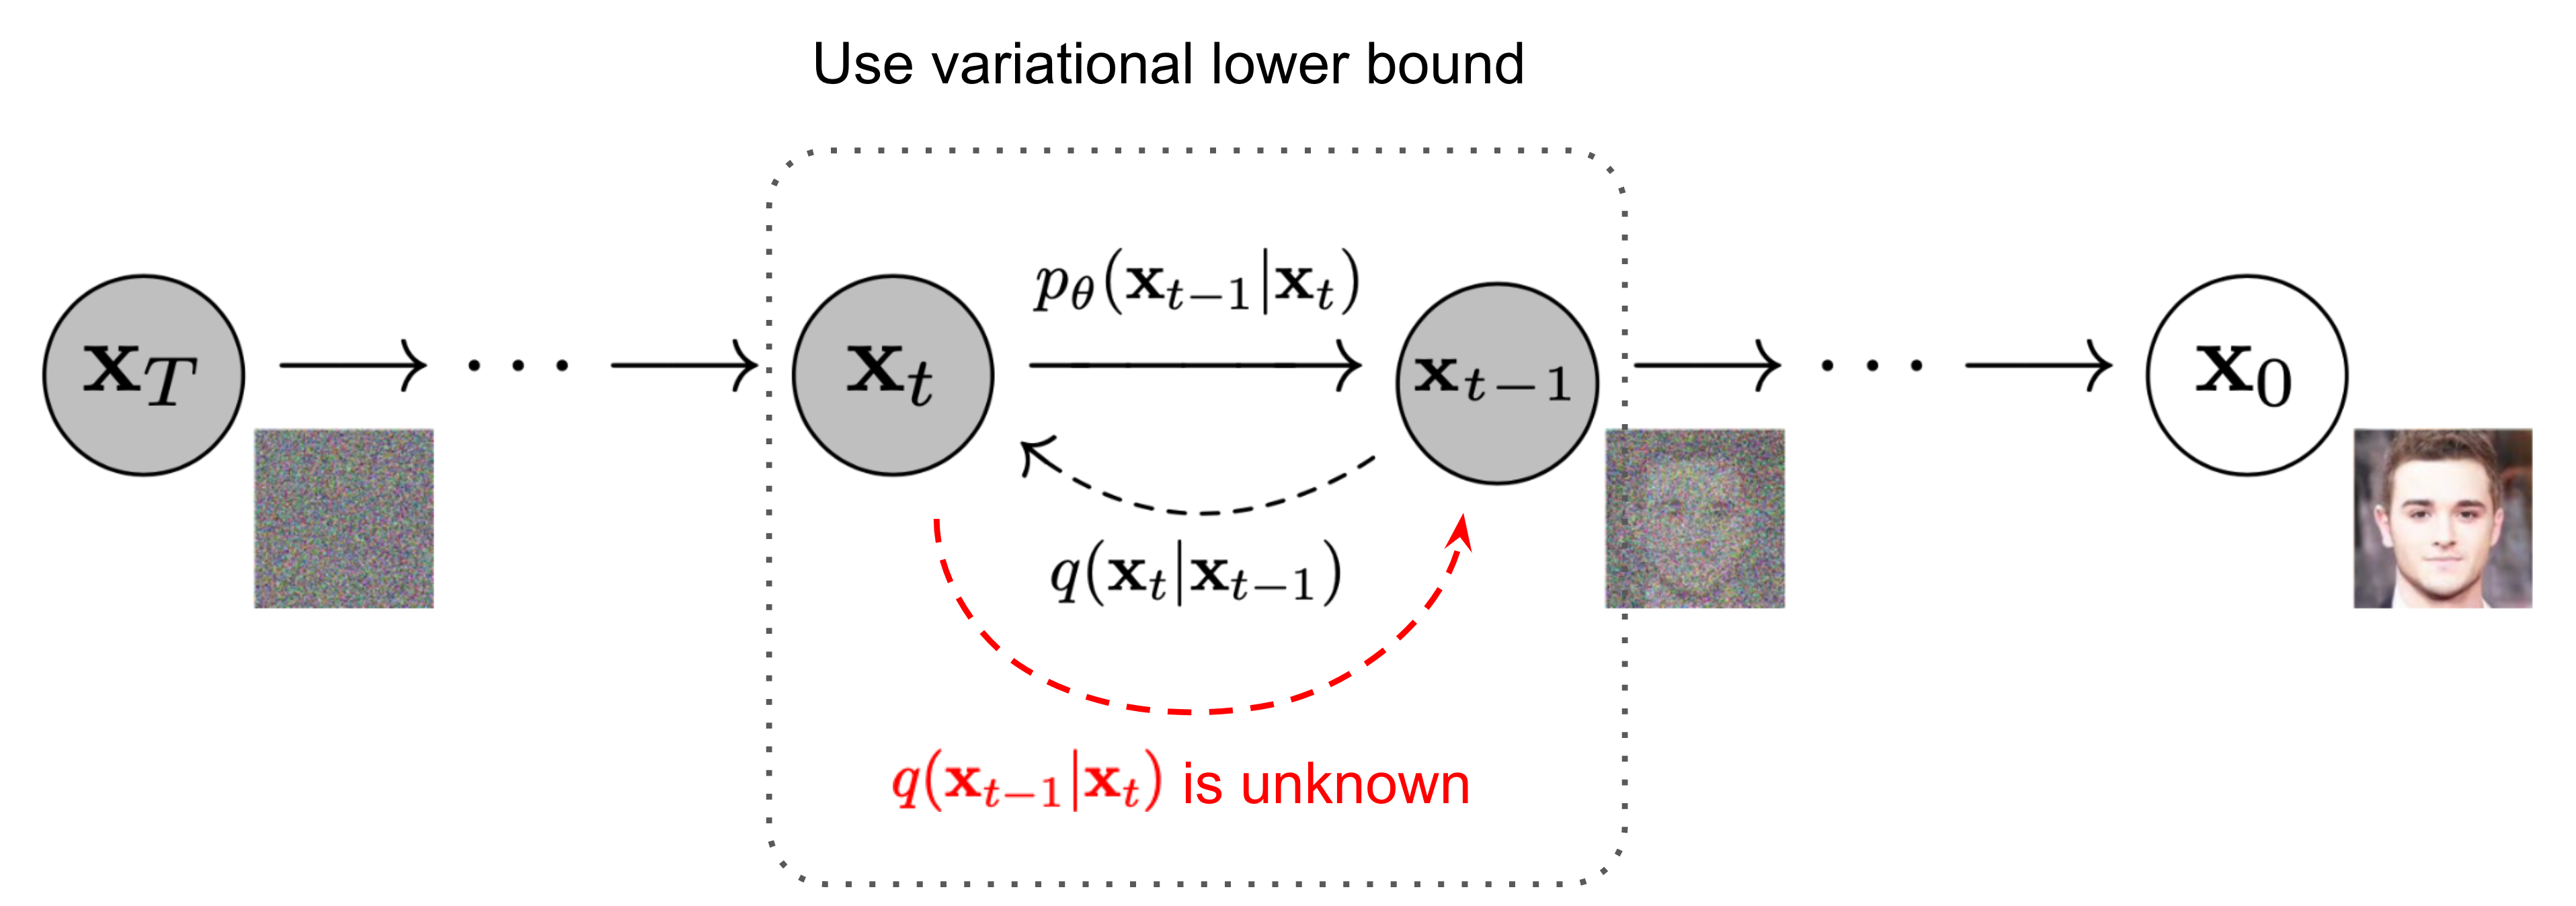
\includegraphics[width=0.9\linewidth]{concept_engineering/ddpm/DDPM.png}
    \caption{Visualization of the diffusion process\cite{ho2020denoisingdiffusionprobabilisticmodels}.}
    \label{fig:diffusion-process}
\end{figure}
Denoising Diffusion Probabilistic Models (DDPM)\cite{ho2020denoisingdiffusionprobabilisticmodels} are generative models that work by gradually adding noise to the data in several steps, and then learning how to reverse this process to recover the original data. The model learns to denoise the image step by step, starting from pure noise and progressively improving its reconstruction until it produces a realistic image. This approach allows DDPM to produce highly detailed synthetic images. 


\paragraph{Loss function}\mbox{}\\
\indent The loss function in DDPM is based on the evidence lower bound (ELBO\footnote{\url{https://en.wikipedia.org/wiki/Evidence_lower_bound}}), also known as "variational lower bound", which involves minimising the difference between the data distribution and the model distribution at each step of the diffusion process. In particular, it includes a term that encourages the model to effectively learn the backward diffusion process.

In practice, ELBO optimization is only the theoretical objective in DDPMs.
\textbf{M}ean \textbf{S}quared \textbf{E}rror and sometimes \textbf{A}bsolute \textbf{E}rror are the practical ways of loss calculation. They are used to calculate an error between added noise and predicted noise. The training objective is to minimize this error. This approach is an approximation of the ELBO optimization.\footnote{Full derivation can be seen in \cite{ho2020denoisingdiffusionprobabilisticmodels} or in this blogpost \url{https://learnopencv.com/denoising-diffusion-probabilistic-models/}}. 

% \begin{equation}
%     \centering
%     L(\theta)=\mathbb{E}_{t, x_0, \epsilon}\left[\left\|\epsilon-\epsilon_\theta\left(x_t, t\right)\right\|^2\right]
%     \label{loss-ddpm}
% \end{equation}

\begin{equation}
\begin{aligned} L_{\text {simple }}(\theta) & :=E_{t \sim U[1, T], \mathbf{x}_0, \epsilon}\left[\left\|\epsilon-\epsilon_\theta\left(\mathbf{x}_t, t\right)\right\|^2\right] \\ & =E_{t \sim U[1, T], \mathbf{x}_0, \epsilon}\left[\left\|\epsilon-\epsilon_\theta\left(\sqrt{\bar{\alpha}_t} \mathbf{x}_0+\sqrt{1-\bar{\alpha}_t} \epsilon, t\right)\right\|^2\right]
\end{aligned}
\end{equation}

where:
\begin{itemize}
    \item $x_0$ - original image,
    \item $T$ - number of timesteps, usually hundreds,
    \item $t$ - particular timestep,
    \item $\epsilon$ - gaussian noise added to original image,
    \item $\theta$ - neural network, for example U-Net,
    \item $\epsilon_\theta(x_t, t)$ - noise predicted by a neural network for a timestep $t$,
    \item $\overline{\alpha_t}$ - scaling factor,
\end{itemize}

The scaling factor is defined as cumulative product of all $\alpha$ between 1 and $t$. 
\begin{equation}
    \overline{\alpha_t} = \prod_{s=1}^t \alpha_s.
\end{equation}

\begin{equation}
    \alpha_t = 1-\beta_t
\end{equation}

The term $\beta_t$ is called "diffusion rate" for timestep $t$ and is calculated using a "noise scheduler". Such scheduler controls how much noise is added to an image in each step. Noise scheduler can be, for example, linear, scaled linear or squared cosine cap.

\paragraph{Training process}\mbox{}\\

\begin{figure}[H]
    \centering
    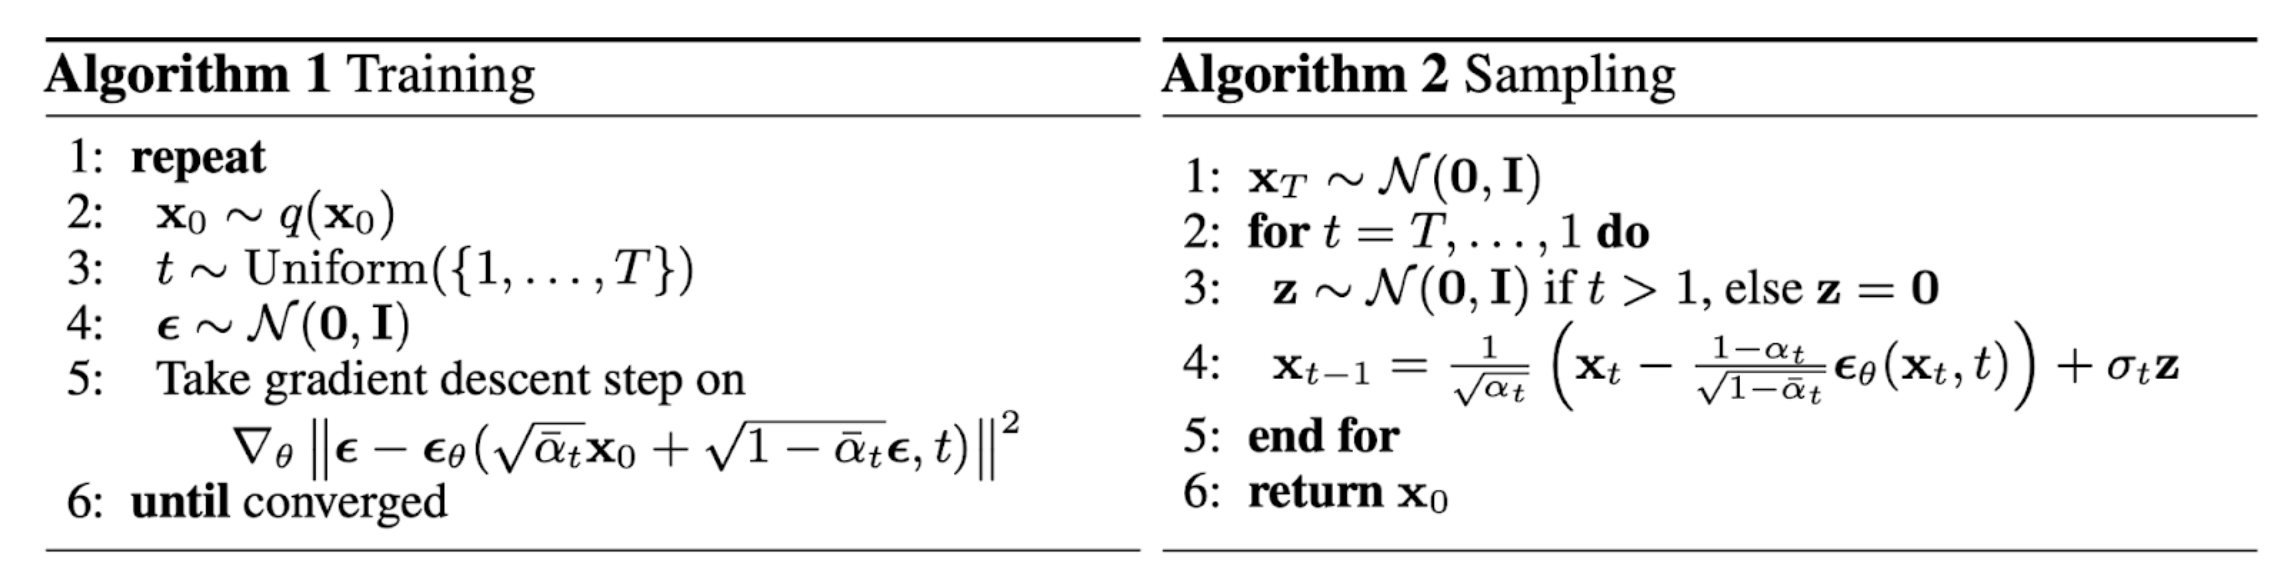
\includegraphics[width=0.9\linewidth]{concept_engineering/ddpm/DDPM-algo.png}
    \caption{Training and sampling algorithms for the diffusion process\cite{ho2020denoisingdiffusionprobabilisticmodels}.}
    \label{fig:diffusion-algo}
\end{figure}
In the training algorithm[\ref{fig:diffusion-algo}] the loss is calculated as a squared error between noise and predicted noise at a timestep $t$. However in practice all squared errors are calculated for each timestep $t$ and then final loss over an image (or a scan in 3D case) is calculated as a mean of these squared errors - MSE. 
This final loss is then aggregated with losses from the whole batch. In this point the gradient is calculated.  

\paragraph{Generation of CT scans}\mbox{}\\
\indent To generate artificial CT scans using DDPM, we could start by sampling gaussian noise and iteratively apply the learned reverse diffusion process. This process should refine the noise into a synthetic CT image that would progressively capture more and more of the anatomical details of the pelvis region.


\paragraph{Latent Diffusion Models}\mbox{}\\
\indent Latent diffusion models are diffusion models but in the latent space of an autoencoder. Unlike original diffusion, they do not generate an image from a Gaussian noise, but they generate its latent representation from a Gaussian noise. Then we can use a decoder to generate an image.
% \begin{figure}
%     \centering
%     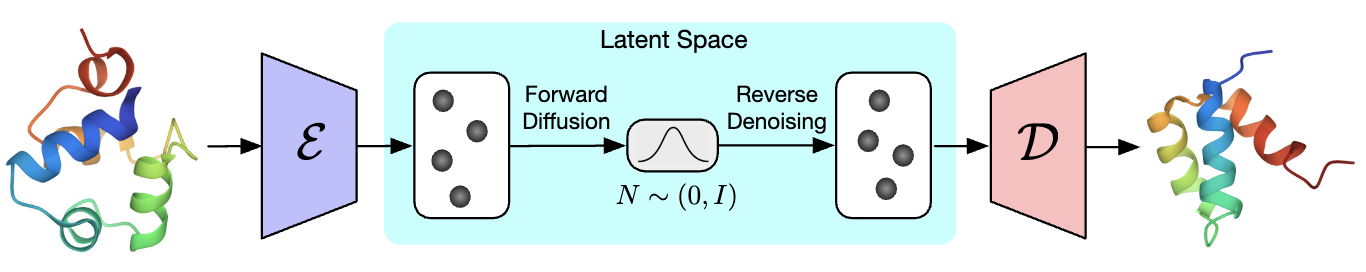
\includegraphics[width=\linewidth]{concept_engineering/ldm/LatentDiff.png}
%     \caption{Caption}
%     \label{fig:enter-label}
% \end{figure}

\begin{figure}[H]
    \centering
    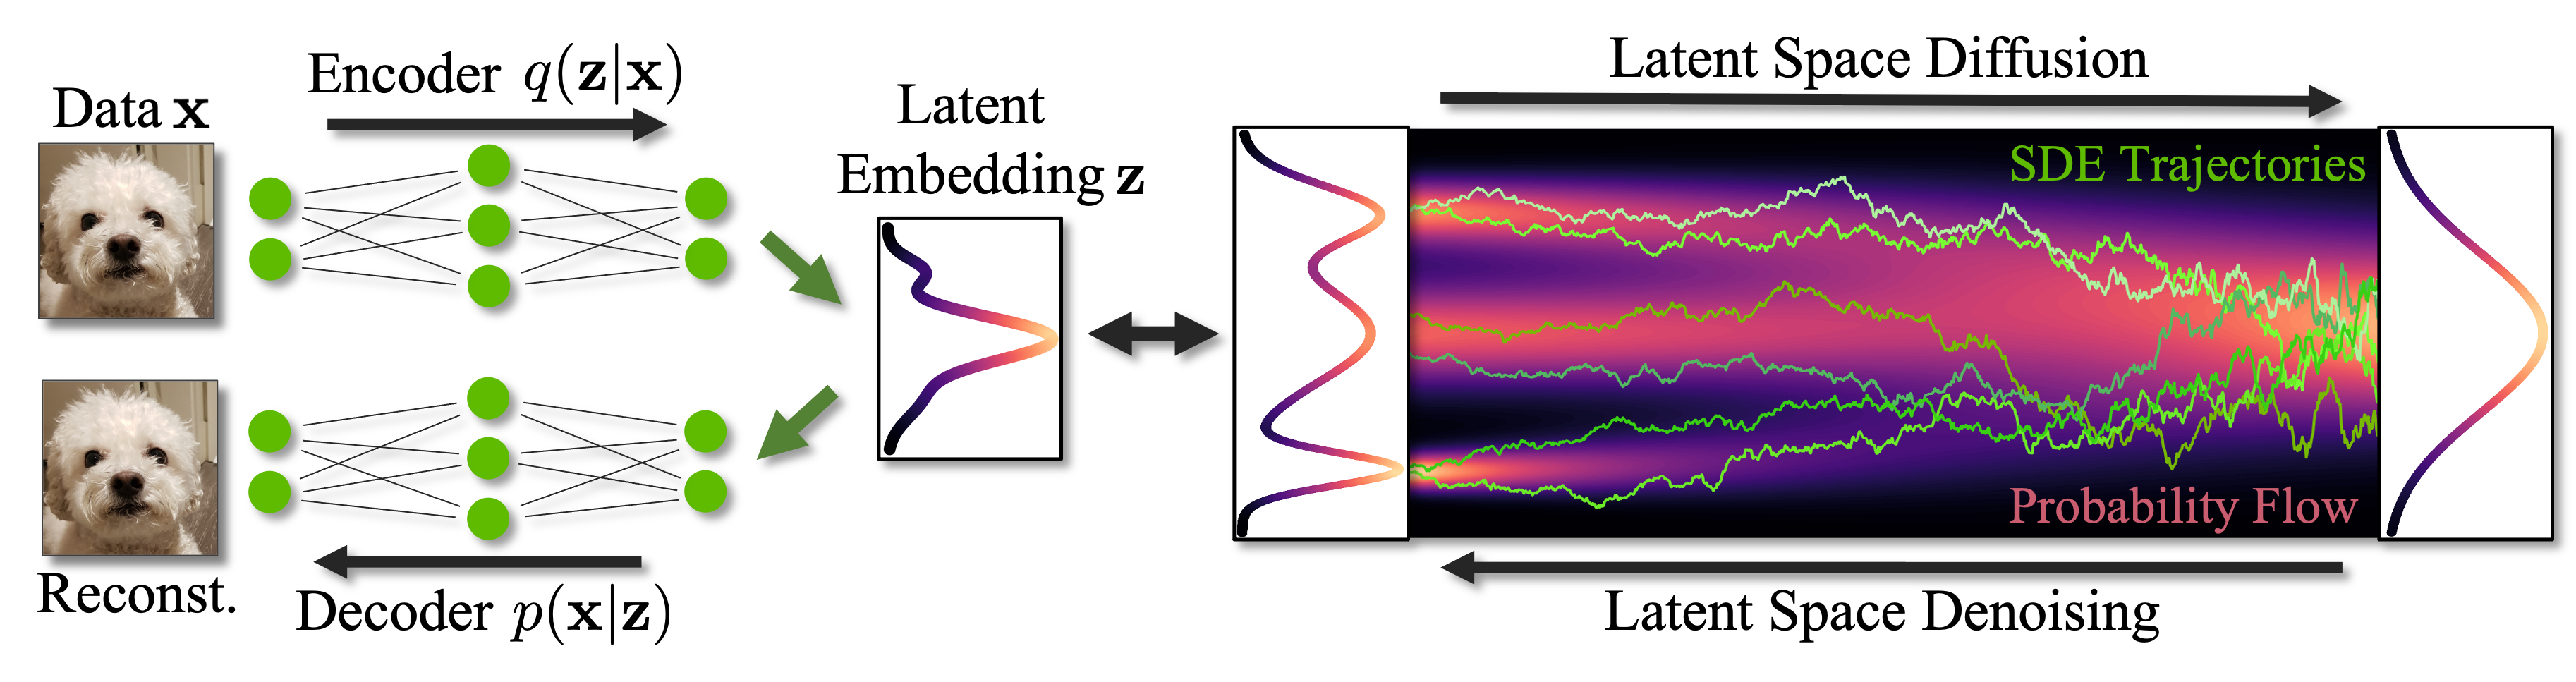
\includegraphics[width=\linewidth]{concept_engineering/ldm/ldm_figure.png}
    \caption{Visualization on how Latent Diffusion Models work. LDM learns latent representations distribution instead of distribution of input data\cite{neurips2023-ldm-tutorial/neurips2023-ldm-tutorial.github.io_2023}.}
    \label{fig:ldm}
\end{figure}

The idea of using diffusion model in the latent space will be used in the architectures below.
More information on LDM can be found on the website\footnote{\url{https://neurips2023-ldm-tutorial.github.io/}} and in the presentation\footnote{\url{https://drive.google.com/file/d/1p_aZ627Bwvku7nKyYRHtfZe50nAnpqGU/view}}.

\newpage
\subsubsection{VAE - Variational Autoencoder}
\begin{figure}[H]
    \centering
    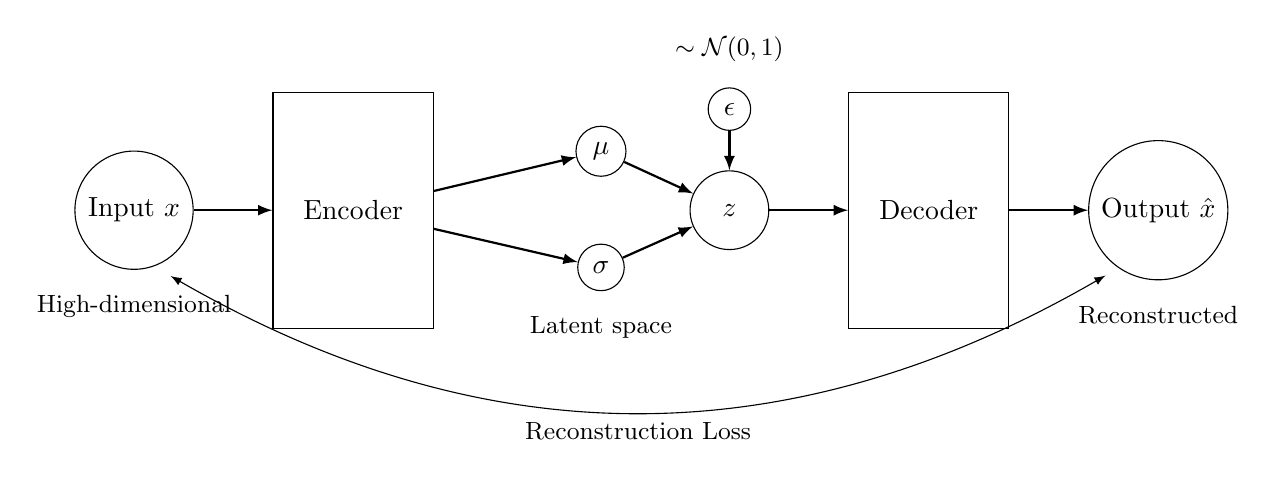
\begin{tikzpicture}[
    box/.style={draw, minimum width=2cm, minimum height=3cm, text width=1.8cm, align=center},
    smallbox/.style={draw, minimum width=1.5cm, minimum height=1.2cm, text width=1.3cm, align=center},
    arrow/.style={->, >=latex, thick},
    label/.style={font=\small}
]

% Components
\node[circle, draw] (input) {Input $x$};
\node[box, right=1cm of input] (encoder) {Encoder};

% Latent space
\node[right=2cm of encoder] (latent) {};
\node[circle, draw, above=0.3cm of latent] (mu) {$\mu$};
\node[circle, draw, below=0.3cm of latent] (sigma) {$\sigma$};
\node[circle, draw, minimum size=1cm, right=1cm of latent] (z) {$z$};

\node[box, right=1cm of z] (decoder) {Decoder};
\node[circle, draw, right=1cm of decoder] (output) {Output $\hat{x}$};

% Reparameterization trick
\node[circle, draw, fill=white, minimum size=0.5cm, above=0.5cm of z] (epsilon) {$\epsilon$};

% Connections
\draw[arrow] (input) -- (encoder);
\draw[arrow] (encoder) -- (mu);
\draw[arrow] (encoder) -- (sigma);
\draw[arrow] (mu) -- (z);
\draw[arrow] (sigma) -- (z);
\draw[arrow] (epsilon) -- (z);
\draw[arrow] (z) -- (decoder);
\draw[arrow] (decoder) -- (output);

% Labels
\node[label, below=0.2cm of input] {High-dimensional};
% \node[label, above=0.2cm of mu] {Latent space};
\node[label, below=0.2cm of sigma] {Latent space};
\node[label, above=0.2cm of epsilon] {$\sim \mathcal{N}(0,1)$};
\node[label, below=0.2cm of output] {Reconstructed};

% % KL Divergence
% \draw[<->, >=latex, bend left=30] ($(encoder.north east)+(0.2,0.2)$) to node[above, font=\small] {KL Divergence} ($(mu.north west)+(-0.2,0.2)$);

% Reconstruction Loss
\draw[<->, >=latex, bend right=30] ($(input.south west)+(1,-0.3)$) to node[below, font=\small] {Reconstruction Loss} ($(output.south east)+(-1.3,-0.2)$);

\end{tikzpicture}
    \caption{Visualization of Variational Autoencoder. Circles are tensors, rectangles are neural networks.}
    \label{fig:vae}
\end{figure}

\indent The main issue with autoencoders in the context of synthetic data generation is that we do not know what values should be assigned to the layer $z$ and passed through decoder in order to obtain meaningful results. The Variational Autoencoder addresses it.
This model extends the standard autoencoder by linking it with probability concepts: mean and standard deviation. VAE learns not only to create a compressed representation of the data, but also a distribution over that representation. This makes VAEs capable of generating new data samples that are similar to those in the training set. Thus, VAE is a suitable choice for image generation, data augmentation, and even anomaly detection.

\begin{figure}[H]
    \centering
    
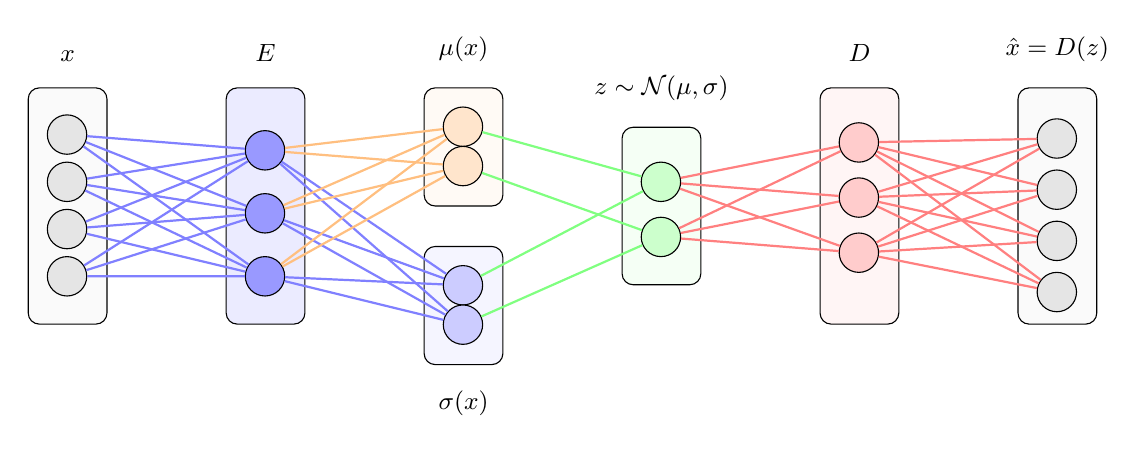
\begin{tikzpicture}[
    neuron/.style={circle, draw, minimum size=0.5cm},
    layer/.style={rectangle, draw, rounded corners, minimum height=3cm, minimum width=1cm, fill opacity=0.2},
    arrow/.style={->, >=latex, thick},
    label/.style={font=\small}
]

% Color definitions
\colorlet{input}{gray!20}
\colorlet{encoder}{blue!40}
\colorlet{mu}{orange!20}
\colorlet{sigma}{blue!20}
\colorlet{latent}{green!20}
\colorlet{decoder}{red!20}

% Input layer
\node[layer, fill=input] (input) {};
\foreach \y in {1,...,4} {
    \node[neuron, fill=input] (i\y) at (input.west |- input.north) [yshift=-\y*0.60cm, xshift=0.5cm] {};
}

% Encoder layer
\node[layer, fill=encoder, right=1.5cm of input] (encoder) {};
\foreach \y in {1,...,3} {
    \node[neuron, fill=encoder] (e\y) at (encoder.west |- encoder.north) [yshift=-\y*0.8cm, xshift=0.5cm] {};
}

% Mu layer
\node[layer, fill=mu, right=1.5cm of encoder, minimum height=1.5cm, yshift=0.75cm] (mu) {};
\foreach \y in {1,...,2} {
    \node[neuron, fill=mu] (mu\y) at (mu.west |- mu.north) [yshift=-\y*0.5cm, xshift=0.5cm] {};
}

% Sigma layer
\node[layer, fill=sigma, below=0.5cm of mu, minimum height=1.5cm] (sigma) {};
\foreach \y in {1,...,2} {
    \node[neuron, fill=sigma] (sigma\y) at (sigma.west |- sigma.north) [yshift=-\y*0.5cm, xshift=0.5cm] {};
}

% Latent layer
\node[layer, fill=latent, right=1.5cm of mu, yshift=-0.75cm, minimum height=2cm] (latent) {};
\foreach \y in {1,...,2} {
    \node[neuron, fill=latent] (l\y) at (latent.west |- latent.north) [yshift=-\y*0.7cm, xshift=0.5cm] {};
}

% Decoder layer
\node[layer, fill=decoder, right=1.5cm of latent] (decoder) {};
\foreach \y in {1,...,3} {
    \node[neuron, fill=decoder] (d\y) at (decoder.west |- decoder.north) [yshift=-\y*0.7cm, xshift=0.5cm] {};
}

% Output layer
\node[layer, fill=input, right=1.5cm of decoder] (output) {};
\foreach \y in {1,...,4} {
    \node[neuron, fill=input] (o\y) at (output.west |- output.north) [yshift=-\y*0.65cm, xshift=0.5cm] {};
}

% Connections
\foreach \i in {1,...,4} {
    \foreach \j in {1,...,3} {
        \draw[blue!50, thick] (i\i) -- (e\j);
    }
}

\foreach \i in {1,...,3} {
    \foreach \j in {1,...,2} {
        \draw[orange!50, thick] (e\i) -- (mu\j);
        \draw[blue!50, thick] (e\i) -- (sigma\j);
    }
}

\foreach \i in {1,...,2} {
    \draw[green!50, thick] (mu\i) -- (l\i);
    \draw[green!50, thick] (sigma\i) -- (l\i);
}

\foreach \i in {1,...,2} {
    \foreach \j in {1,...,3} {
        \draw[red!50, thick] (l\i) -- (d\j);
    }
}

\foreach \i in {1,...,3} {
    \foreach \j in {1,...,4} {
        \draw[red!50, thick] (d\i) -- (o\j);
    }
}

% Labels
\node[label, above=0.2cm of input] {$x$};
\node[label, above=0.2cm of encoder] {$E$};
\node[label, above=0.2cm of mu] {$\mu(x)$};
\node[label, below=0.2cm of sigma] {$\sigma(x)$};
\node[label, above=0.2cm of latent] {$z \sim \mathcal{N}(\mu, \sigma)$};
\node[label, above=0.2cm of decoder] {$D$};
\node[label, above=0.2cm of output] {$\hat{x} = D(z)$};

\end{tikzpicture}
    \caption{Visualization of a simple VAE.}
    \label{fig:vae-simple}
\end{figure}

The figure[\ref{fig:vae-simple}] shows detailed visualization of a simple Variational Autoencoder. It is worth noticing that the encoder $E$ has two outputs, $\mu$ and $\sigma$, which produce $z$ using the reparameterization trick\footnote{\url{https://www.baeldung.com/cs/vae-reparameterization}}.

\begin{equation}
    z = \mu + \sigma\cdot\epsilon,
\end{equation}

where $\epsilon\sim\mathcal{N}(0,1)$.

\paragraph{Loss Function:}\mbox{}\\
The VAE loss is a combination of:
\begin{enumerate}
\item \textbf{Reconstruction Loss}, which ensures how well the reconstructed image matches the original input image, for example $L1$, $L2$, $MSE$,
\item \textbf{KL Divergence Loss} that ensures the latent space follows a Gaussian distribution.
\end{enumerate}

\begin{equation}
    L = L_{reconstruction} + \mathbb{KL}(q(z | x) || p(z)),
\end{equation}

where 
\begin{itemize}
    \item $\mathbb{KL}$ - Kullback-Leibler divergence\footnote{\url{https://en.wikipedia.org/wiki/Kullback\%E2\%80\%93Leibler_divergence}}, measures how much two distributions differ from each other,
    \item $q(z | x) = \mathcal{N}(\mu, \sigma)$ - probability distribution of the latent representation $z$, in other words probability distribution of endocers output,
    \item $p(z) = \mathcal{N}(0,1)$ - expected probability distribution.
\end{itemize}

After substituting probabilities, the loss $L$ becomes\footnote{Broader explanation and Pytorch toy example can be found here \url{https://avandekleut.github.io/vae/}.}
\begin{equation}
    L = L_{reconstruction} + \mathbb{KL}(\mathcal{N}(\mu,\sigma), \mathcal{N}(0,1)).
\end{equation}

The difference between two Gaussians can be calculated using the identity\cite{7449}. 

\begin{equation}
    \mathbb{KL}\left( \mathcal{N}(\mu, \sigma) \parallel \mathcal{N}(0, 1) \right) = \sum_{x \in X} \left( \sigma^2 + \mu^2 - \log \sigma - \frac{1}{2} \right)
\end{equation}


% Train the VAE on prostate CT scans to learn an efficient latent space representation.
\paragraph{Generation of CT scans}\mbox{}\\

To generate new CT scans, we could sample the Gaussian noise tensor of shape $z$, which follows the normal distribution, and then pass it through the decoder.
If the model is properly trained, the decoder should reconstruct this latent representation into a realistic synthetic CT image. 

However, it is not guaranteed that the learned distribution $q(z)$ is always similar to $\mathbf{N}(0,1)$, especially when the $\mathbb{KL}$ loss is far from $0$. To mitigate this issue, aggregated posterior probability could be used. For example, by passing the entire dataset through the encoder and averaging resulted in $\mu$s to $\overline{\mu}$ and $\sigma$s to $\overline{\sigma}$ and then sampling from $\mathcal{N}(\overline{\mu}, \overline{\sigma})$. The alternative solution is to train another neural network that would learn the distribution of the latent representation of $z$ - $q(z)$. Such a neural network could be a Latent Diffusion Model described in the previous section.

% ### Key Differences from Traditional Autoencoders

% ### VAE Structure

% 1. **Encoder (Inference Network)**: The encoder maps an input \( x \) to a latent representation, but instead of outputting a single value, it outputs parameters of a probability distribution, typically a Gaussian distribution with a mean \( \mu \) and a variance \( \sigma^2 \). This is achieved by splitting the encoder's output into two parts:

% \[
% q(z|x) = \mathcal{N}(z; \mu(x), \sigma^2(x))
% \]

% where:
% - \( \mu(x) \) is the mean of the latent distribution for input \( x \),
% - \( \sigma^2(x) \) is the variance of the latent distribution for input \( x \),
% - \( z \) is the latent variable sampled from the distribution \( q(z|x) \).

% 2. **Reparameterization Trick**: To allow backpropagation through the stochastic sampling process, VAEs use the reparameterization trick. Instead of sampling \( z \) directly from \( \mathcal{N}(\mu(x), \sigma^2(x)) \), a random variable \( \epsilon \sim \mathcal{N}(0, 1) \) is sampled, and \( z \) is computed as:

% \[
% z = \mu(x) + \sigma(x) \cdot \epsilon
% \]

% This trick makes the sampling process differentiable, enabling gradient-based optimization.

% 3. **Decoder (Generative Network)**: The decoder reconstructs the input data from the latent variable \( z \). The decoder maps \( z \) back to the data space, producing a reconstruction \( \hat{x} \). Similar to traditional autoencoders, this is done through a neural network.

% ### VAE Loss Function

% The loss function in a VAE consists of two terms:

% 1. **Reconstruction Loss**: This measures how well the decoder can reconstruct the input from the latent variable \( z \). It is typically the Mean Squared Error (MSE) or binary cross-entropy, depending on the nature of the data:

% \[
% L_{reconstruction} = \mathbb{E}_{q(z|x)} [||x - \hat{x}||^2]
% \]

% 2. **KL Divergence (Regularization Term)**: The second term ensures that the learned latent distribution \( q(z|x) \) is close to a chosen prior distribution \( p(z) \) (usually a standard normal distribution \( \mathcal{N}(0, 1) \)). This regularization term is the Kullback-Leibler (KL) divergence between the approximate posterior \( q(z|x) \) and the prior \( p(z) \):

% \[
% D_{KL}(q(z|x) || p(z)) = \frac{1}{2} \sum_{i=1}^n (1 + \log(\sigma_i^2) - \mu_i^2 - \sigma_i^2)
% \]

% The total VAE loss is a combination of the reconstruction loss and the KL divergence:

% \[
% L_{VAE} = L_{reconstruction} + D_{KL}(q(z|x) || p(z))
% \]

% This loss encourages the model to reconstruct the input data accurately while ensuring that the latent variables follow the prior distribution.

% ### Applications

% 1. **Data Generation**: By sampling latent vectors from the learned distribution, VAEs can generate new data points similar to those in the training set.
   
% 2. **Anomaly Detection**: VAEs can detect anomalies by measuring the reconstruction error for unseen data; higher reconstruction errors often indicate anomalies.
   
% 3. **Data Augmentation**: VAEs can be used to generate additional synthetic data for training, improving model generalization.

% 4. **Latent Space Exploration**: The continuous and smooth latent space learned by VAEs allows for meaningful interpolations between data points.

% ---

% **References**:
% 1. Kingma, D. P., & Welling, M. (2013). *Auto-Encoding Variational Bayes*. arXiv preprint arXiv:1312.6114.
% 2. Doersch, C. (2016). *Tutorial on Variational Autoencoders*. arXiv preprint arXiv:1606.05908.
% 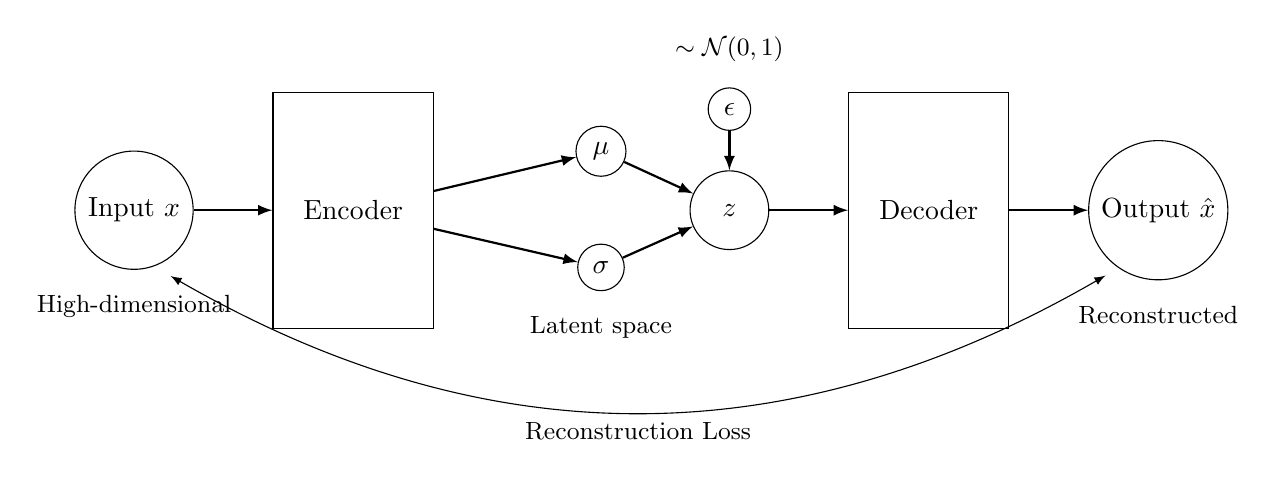
\begin{tikzpicture}[
    box/.style={draw, minimum width=2cm, minimum height=3cm, text width=1.8cm, align=center},
    smallbox/.style={draw, minimum width=1.5cm, minimum height=1.2cm, text width=1.3cm, align=center},
    arrow/.style={->, >=latex, thick},
    label/.style={font=\small}
]

% Components
\node[circle, draw] (input) {Input $x$};
\node[box, right=1cm of input] (encoder) {Encoder};

% Latent space
\node[right=2cm of encoder] (latent) {};
\node[circle, draw, above=0.3cm of latent] (mu) {$\mu$};
\node[circle, draw, below=0.3cm of latent] (sigma) {$\sigma$};
\node[circle, draw, minimum size=1cm, right=1cm of latent] (z) {$z$};

\node[box, right=1cm of z] (decoder) {Decoder};
\node[circle, draw, right=1cm of decoder] (output) {Output $\hat{x}$};

% Reparameterization trick
\node[circle, draw, fill=white, minimum size=0.5cm, above=0.5cm of z] (epsilon) {$\epsilon$};

% Connections
\draw[arrow] (input) -- (encoder);
\draw[arrow] (encoder) -- (mu);
\draw[arrow] (encoder) -- (sigma);
\draw[arrow] (mu) -- (z);
\draw[arrow] (sigma) -- (z);
\draw[arrow] (epsilon) -- (z);
\draw[arrow] (z) -- (decoder);
\draw[arrow] (decoder) -- (output);

% Labels
\node[label, below=0.2cm of input] {High-dimensional};
% \node[label, above=0.2cm of mu] {Latent space};
\node[label, below=0.2cm of sigma] {Latent space};
\node[label, above=0.2cm of epsilon] {$\sim \mathcal{N}(0,1)$};
\node[label, below=0.2cm of output] {Reconstructed};

% % KL Divergence
% \draw[<->, >=latex, bend left=30] ($(encoder.north east)+(0.2,0.2)$) to node[above, font=\small] {KL Divergence} ($(mu.north west)+(-0.2,0.2)$);

% Reconstruction Loss
\draw[<->, >=latex, bend right=30] ($(input.south west)+(1,-0.3)$) to node[below, font=\small] {Reconstruction Loss} ($(output.south east)+(-1.3,-0.2)$);

\end{tikzpicture}
% Reparametrization trick


% 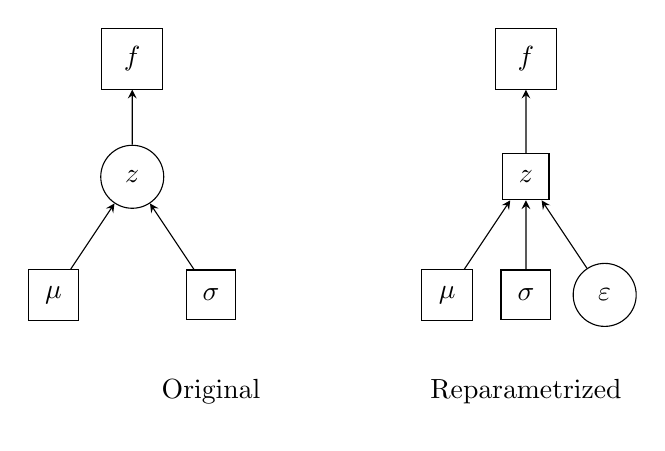
\begin{tikzpicture}[
    node distance = 1cm and 2cm,
    every node/.style = {draw, minimum size=0.8cm},
    % square/.style = {sides=4},
    square/.style = {regular polygon,regular polygon sides=4},
    arr/.style = {->, >=stealth}
]

% Original graph
\node[square] (f1) at (0,0) {$f$};
\node[circle] (z1) at (0,-1.5) {$z$};
\node[square] (mu1) at (-1,-3) {$\mu$};
\node[square] (sigma1) at (1,-3) {$\sigma$};

\draw[arr] (mu1) -- (z1);
\draw[arr] (sigma1) -- (z1);
\draw[arr] (z1) -- (f1);

\node[below=0.5cm of sigma1, draw=none] {Original};

% Reparametrized graph
\node[square] (f2) at (5,0) {$f$};
\node[square] (z2) at (5,-1.5) {$z$};
\node[square] (mu2) at (4,-3) {$\mu$};
\node[square] (sigma2) at (5,-3) {$\sigma$};
\node[circle] (epsilon) at (6,-3) {$\varepsilon$};

\draw[arr] (mu2) -- (z2);
\draw[arr] (sigma2) -- (z2);
\draw[arr] (epsilon) -- (z2);
\draw[arr] (z2) -- (f2);

\node[below=0.5cm of sigma2, draw=none] {Reparametrized};

\end{tikzpicture}

\newpage
\subsubsection{VQVAE}
% 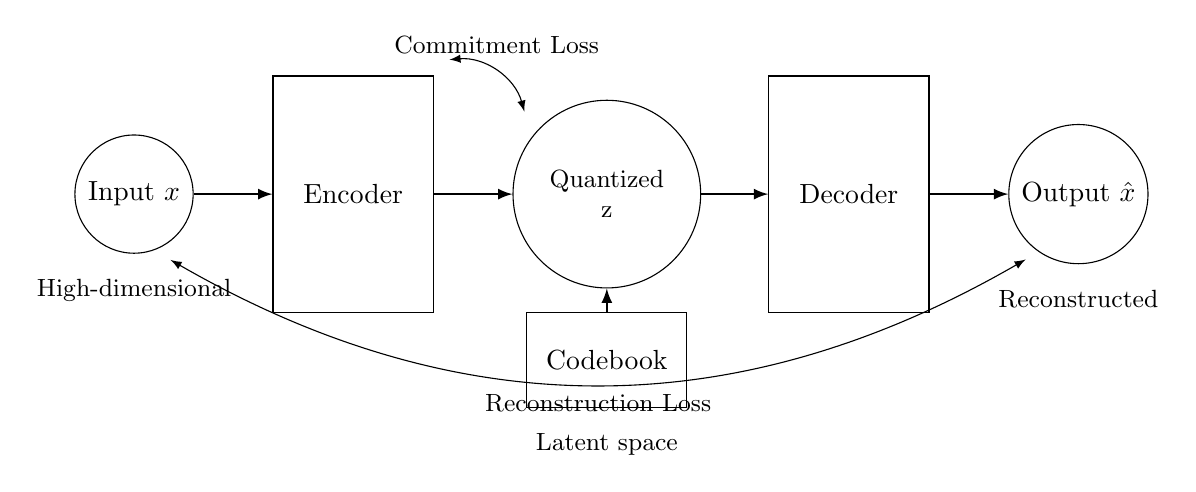
\begin{tikzpicture}[
    box/.style={draw, minimum width=2cm, minimum height=3cm, text width=1.8cm, align=center},
    smallbox/.style={draw, minimum width=1.5cm, minimum height=1.2cm, text width=1.8cm, align=center},
    arrow/.style={->, >=latex, thick},
    label/.style={font=\small},
    % circle/.style={draw, align=center}
]

% Components
\node[circle, draw] (input) {Input $x$};
\node[box, right=1cm of input] (encoder) {Encoder};

% Latent space
\node[right=2cm of encoder] (latent) {};
\node[circle, draw, right=1cm of encoder, font=\small, align=center,text width=2cm] (quantized) {Quantized \\ z};
\node[smallbox, below=0.3cm of quantized] (codebook) {Codebook};

\node[box, right=2cm of latent] (decoder) {Decoder};
\node[circle, draw, right=1cm of decoder] (output) {Output $\hat{x}$};

% Connections
\draw[arrow] (input) -- (encoder);
\draw[arrow] (encoder) -- (quantized);
\draw[arrow] (codebook) -- (quantized);
\draw[arrow] (quantized) -- (decoder);
\draw[arrow] (decoder) -- (output);

% Labels
\node[label, below=0.2cm of input] {High-dimensional};
\node[label, below=0.2cm of codebook] {Latent space};
\node[label, below=0.2cm of output] {Reconstructed};

% Reconstruction Loss
\draw[<->, >=latex, bend right=30] ($(input.south west)+(1,-0.3)$) to node[below, font=\small] {Reconstruction Loss} ($(output.south east)+(-1.3,-0.2)$);

% Commitment Loss
\draw[<->, >=latex, bend left=40] ($(encoder.north east)+(0.2,0.2)$) to node[above=0.1cm, font=\small] {Commitment Loss} ($(quantized.north west)+(-0.2,0.2)$);

\end{tikzpicture}
\begin{figure}[H]
    \centering
    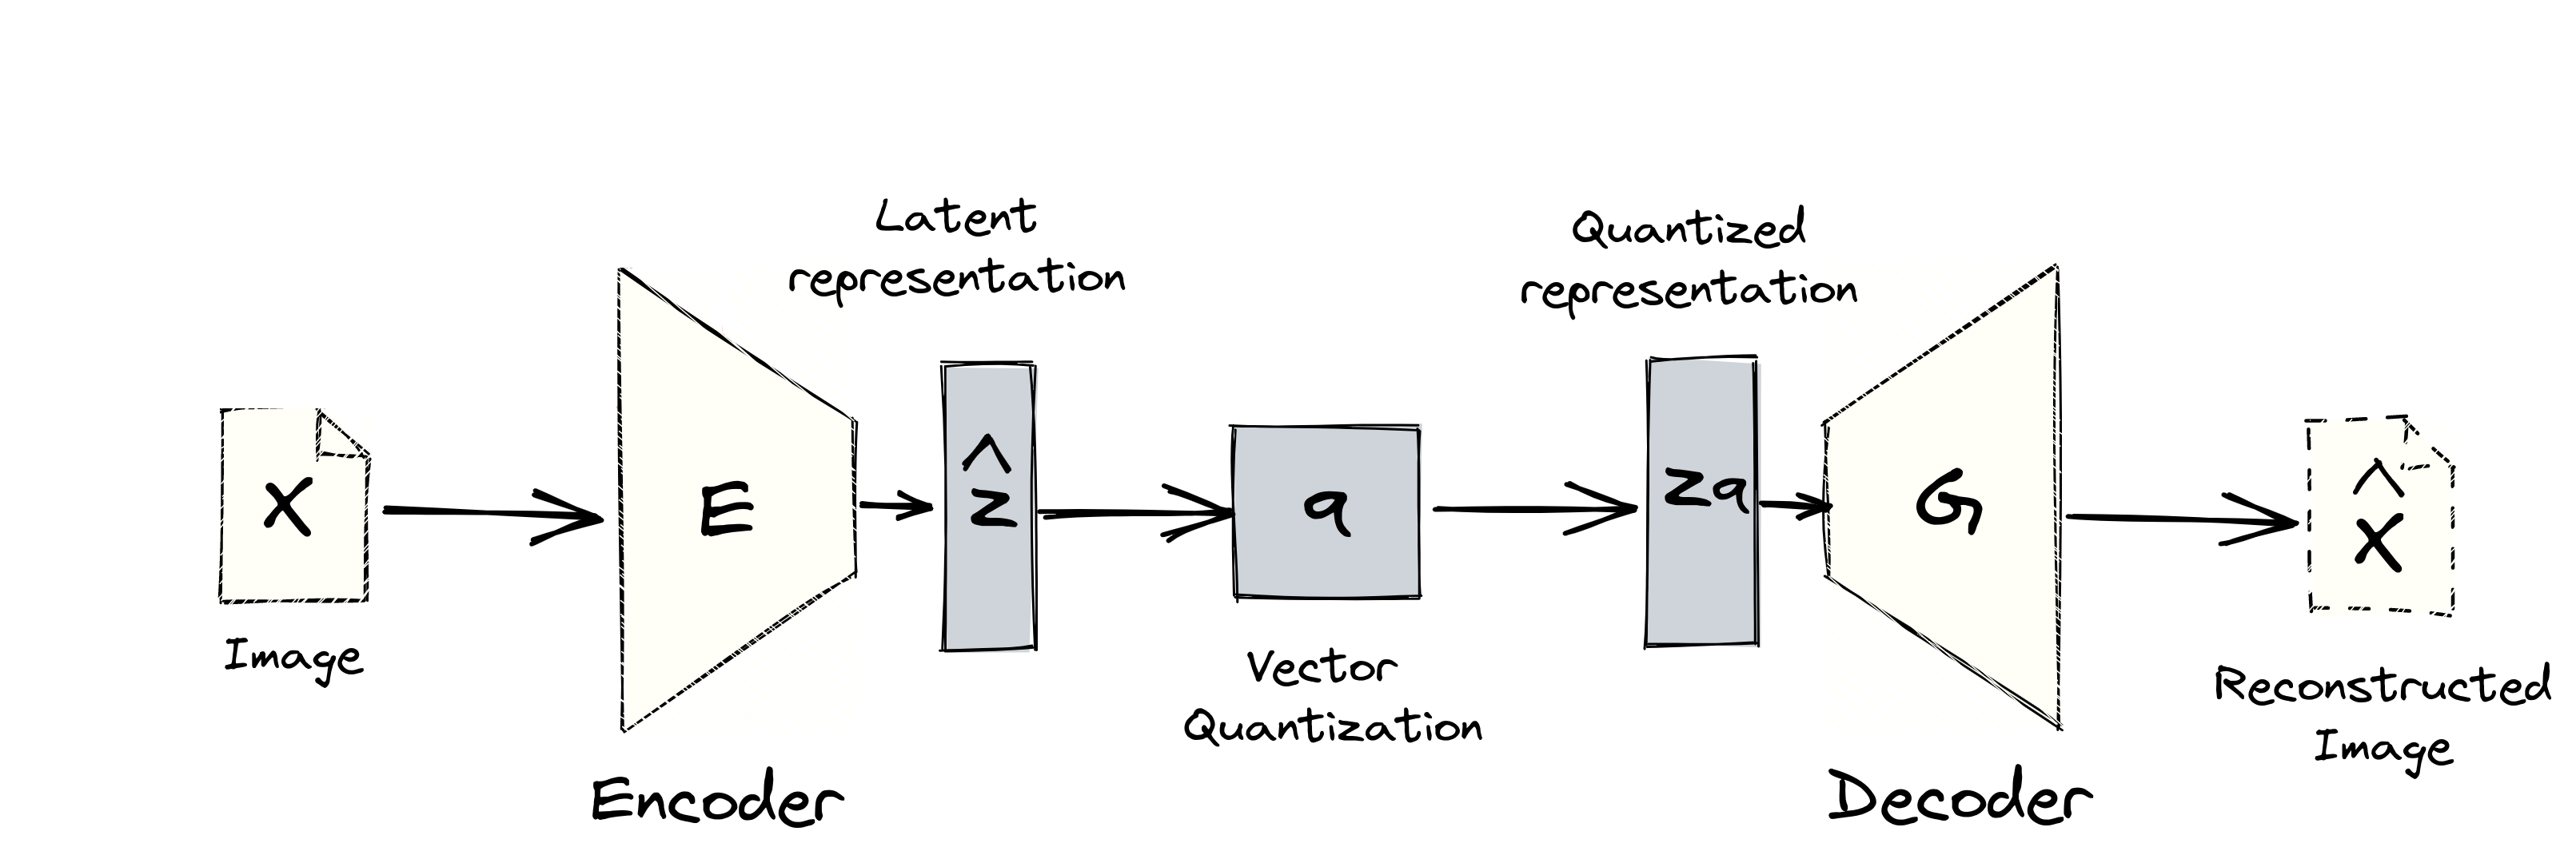
\includegraphics[width=\linewidth]{concept_engineering/vqgan/vqvae.png}
    \caption{Visualization of Vector Quantized Variational Autoencoder\cite{miranda2021vqgan}.}
    \label{fig:vavae1}
\end{figure}

The variational autoencoders latent representation $z$ can have any value, usually from the distribution $\sim \mathbb{N}(0,1)$. Unfortunately, it sometimes leads to posterior collapse. This means that the decoder starts to treat latent representation $z$ as meaningless noise and ignores it. Instead, it learns to encode the dataset in itself. When something like this happens decoder cannot generate meaningful results, no matter the given $z$. 

\begin{figure}[H]
    \centering
    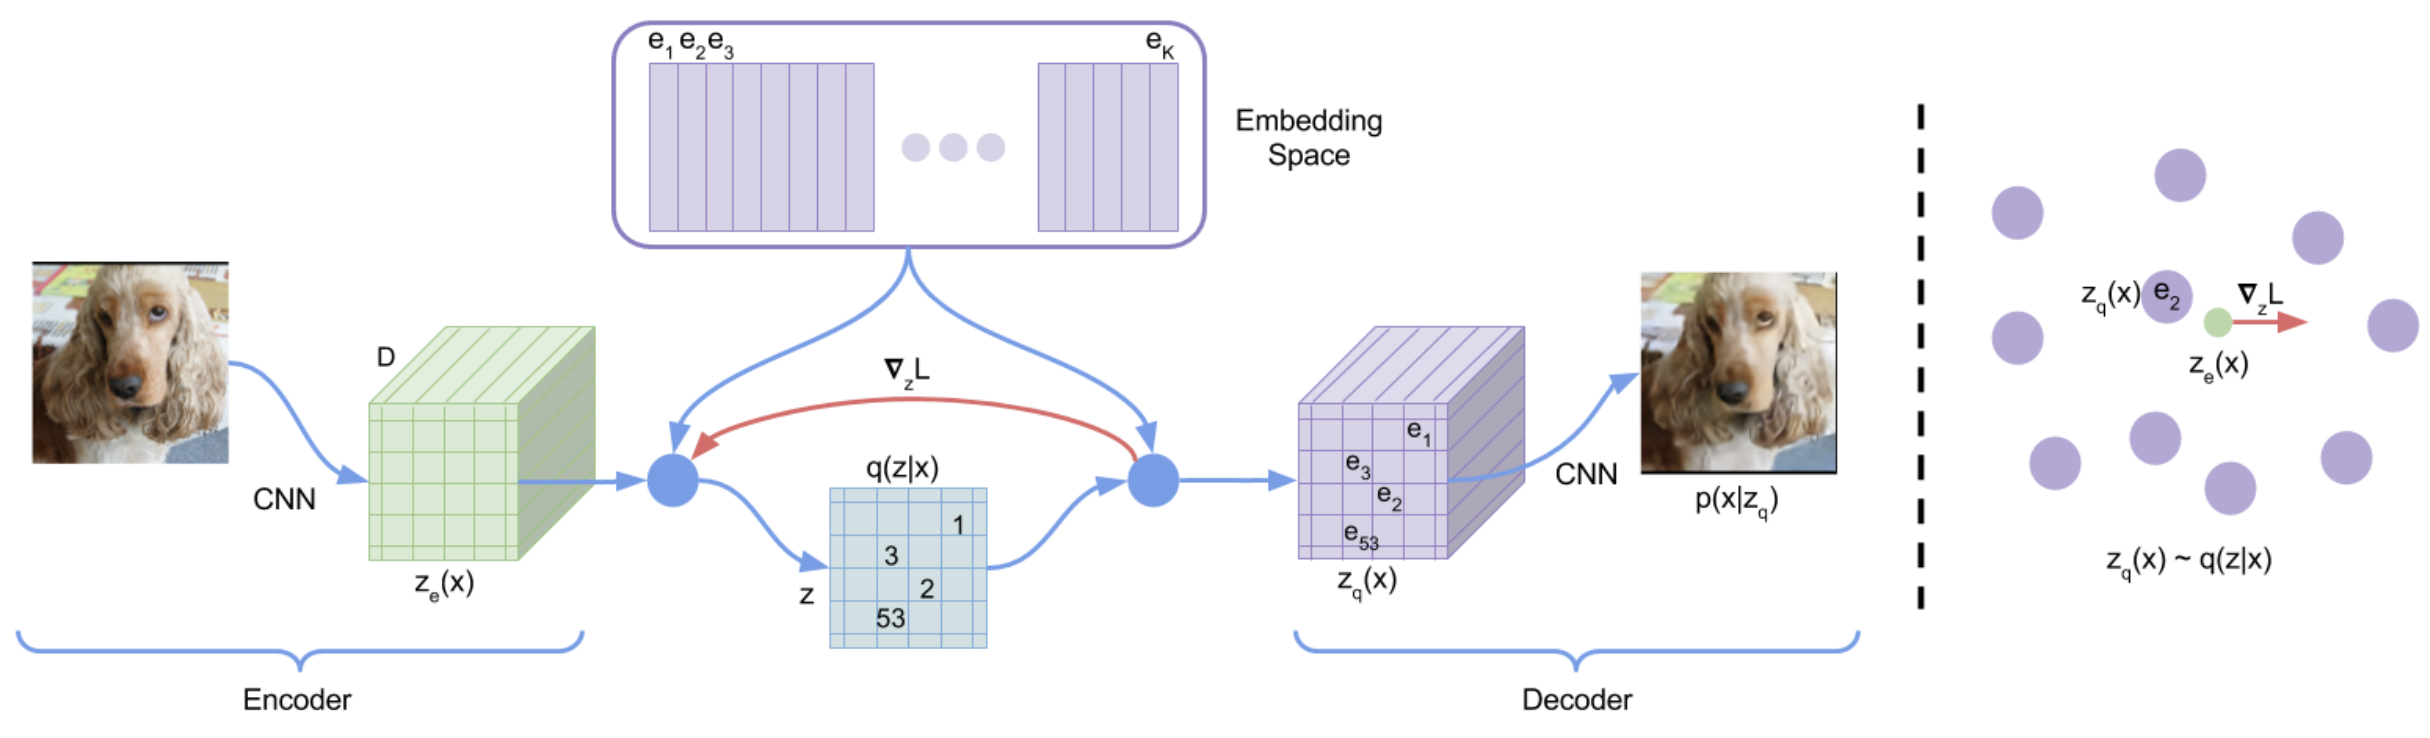
\includegraphics[width=\linewidth]{concept_engineering/vqvae.png}
    \caption{VQVAE visualization showing compression of an image to latent representation (a cube), encoding and decompression\cite{oord2018neuraldiscreterepresentationlearning}.}
    \label{fig:vqvae-paper}
\end{figure}

To mitigate this issue, researchers\cite{oord2018neuraldiscreterepresentationlearning} came up with the idea of having a fixed set of latent representations that hold semantic meaning. In case of images, the encoder compresses the original image of dimensions $(C,H,W)$ to its latent representation $(D,H_2,W_2)$ (a tensor "cube"), where $C<D$, $H>H_2$ and $W>W_2$. Then each latent "pixel" (a cell on a figure\ref{fig:vqvae-paper}) gets a vector from the codebook that holds the semantic meaning of this part of the compressed image. 

%the image to codes from the codebook and then uses the decoder to retrieve the original value. 

\paragraph{Loss function}\mbox{}\\
% Reconstruction Loss (between input and output) and Commitment Loss (penalizing the difference between encoder outputs and quantized embeddings).
The VQVAE loss has three parts.

\begin{itemize}
    \item \textbf{Reconstruction loss} the same as in the VAE, measures how ensures the output matches the input.
    \item \textbf{Commitment loss} - penalizes the difference between encoder outputs and quantized embeddings,
    \item \textbf{Codebook loss} - it is the same value as commitment loss, however it is used to change values of codebook representations through backpropagation.
\end{itemize}

which can be expressed by this formula
\begin{equation}
    L_{VQ}(E, G, Z) = \underbrace{||x-\hat{x}||^{2}}_{\text{reconstruction loss}} + \underbrace{||sg[E(x)] - z_\mathbf{q}||_2^2}_{\text{codebook loss}}
+ \underbrace{||sg[z_\mathbf{q}] - E(x) ||_{2}^2}_{\text{commitment loss}},
    \label{loss_vq}
\end{equation}

where
\begin{itemize}
    \item $\hat{x}$ - reconstructed image,
    \item $E(x)=\hat{z}$ - encoder output,
    \item $z_\mathbf{q}$ - quantized $\hat{z}$,
    \item $sg$ - stop gradient.
\end{itemize}

VQVAE models have one important metric to note - Perplexity. It measures utilization of the codebook during embeeding. Higher is better.

% Codebook Loss: Ensures the quantized latent vectors match the encoder output.
% The commitment loss encourages the encoder to use the codebook efficiently.
\paragraph{Generation of CT scans}\mbox{}\\
\indent Unlike in case of VAE, the probability distribution $q(z_e|x)$ is not conditioned to be close to $\mathcal{N}(0,1)$. Thus, to generate a new image, one cannot just pass a Gaussian noise tensor through the codebook and decoder.
Instead, after successful training of VQVAE, another model like LDM should be used to learn to generate $z_e$ from Gaussian noise.

After that, to generate a synthetic CT scan, one can generate a tensor $z$ of Gaussian noise and then pass it through the denoising LDM to obtain $z_e$. Next, the closest codebook vector should be chosen for each "hidden pixel", for example using L1, L2 or MSE. After that, one would obtain $z_q$, which should then pass through the decoder to obtain the synthetic image.


% should be created and used to select the closest latent code from the codebook. Then the retrieved latent code should be passed through the decoder in order to transform it into a synthetic CT image.

% The target is to:
% $$ (\phi,\theta)=\underset{\phi,\theta}{\mathrm{argmax}}\quad\sum_{\mathbf{x}\in\mathcal{X}}\mathrm{ELBO}(\mathbf{x}), $$

% $$ \begin{aligned}\nabla_{\boldsymbol{\theta},\boldsymbol{\phi}}\:\mathrm{ELBO}(\mathbf{x}) & =\nabla_{\boldsymbol{\theta},\boldsymbol{\phi}}\left\{\mathbb{E}_{q_{\phi}(\mathbf{z}|\mathbf{x})}\left[\log\frac{p_{\boldsymbol{\theta}}(\mathbf{x},\mathbf{z})}{q_{\boldsymbol{\phi}}(\mathbf{z}|\mathbf{x})}\right]\right\}\\  & =\nabla_{\boldsymbol{\theta},\boldsymbol{\phi}}\Big{\{}\mathbb{E}_{q_{\mathrm{o}}(\mathbf{z}|\mathbf{x})}\Big{[}\log p_{\boldsymbol{\theta}}(\mathbf{x},\mathbf{z})-\log q_{\boldsymbol{\phi}}(\mathbf{z}|\mathbf{x})\Big{]}\Big{\}}.\end{aligned} $$

% $$ (\boldsymbol{\mu},\boldsymbol{\sigma}^2)=\mathrm{EncoderNetwork}_{\boldsymbol{\phi}}(\mathbf{x})\\q_{\phi}(\mathbf{z}|\mathbf{x})=\mathcal{N}(\mathbf{z}\mid\boldsymbol{\mu},\mathrm{diag}(\boldsymbol{\sigma}^2)) $$

% $$ (\boldsymbol{\mu},\sigma^2)=\mathrm{EncoderNetwork}_{\boldsymbol{\phi}}(\mathbf{x})q_{\phi}(\mathbf{z}|\mathbf{x})=\mathcal{N}(\mathbf{z}\mid\mathbf{\mu},\sigma^2\mathbf{I} $$

% $$ \begin{aligned}\mu & =\underbrace{\mu_{\phi}}_{\text{neural network}}(\mathbf{x}),\\ \sigma^2 & =\underbrace{\sigma_{\phi}^2}_{\text{neural network}}(\mathbf{x}),\end{aligned} $$


% $$ \begin{aligned}\mathrm{ELBO}_{\boldsymbol{\phi},\boldsymbol{\theta}}(\mathbf{x}) & =\mathbb{E}_{q_{\boldsymbol{\phi}}(\mathbf{x}_1|\mathbf{x}_0)}\Big{[}\log\underbrace{p_{\boldsymbol{\theta}}(\mathbf{x}_0|\mathbf{x}_1)}_{\mathrm{how~good~the~tintial~block~is}}\Big{]}\\  & -\mathbb{E}_{q_{\boldsymbol{\phi}}(\mathbf{x}_{T-1}|\mathbf{x}_0)}\Big{[}\underbrace{\mathbb{D}_{\mathrm{KL}}\Big{(}q_{\boldsymbol{\phi}}(\mathbf{x}_{T}|\mathbf{x}_{T-1})\|p(\mathbf{x}_{T})\Big{)}\Big{]}}_{\mathrm{how~good~the~final~block~is}}\Big{]}\\  & -\sum_{t=1}^{T-1}\mathbb{E}_{q_{\boldsymbol{\theta}}(\mathbf{x}_{t-1},\mathbf{x}_{t+1}|\mathbf{x}_0)}\Big{[}\underbrace{\mathbb{D}_{\mathrm{KL}}\Big{(}q_{\boldsymbol{\phi}}(\mathbf{x}_{t}|\mathbf{x}_{t-1})\|p_{\boldsymbol{\theta}}(\mathbf{x}_{t}|\mathbf{x}_{t+1})\Big{)}}_{\mathrm{how~good~the~transition~blocks~are}}\Big{]},\end{aligned} $$

\newpage
\subsubsection{VQGAN} 
VQGAN proposed in \cite{Esser_2021_CVPR} is a hybrid model that combines VQVAE's structured latent space with GANs. VQGAN can create high-quality images by using GANs to make textures and details look more realistic.
% This technique, in comparison to the direct use of diffusion models to 3D data, allows one to train a model using less computational resources and sampling from compressed latent space that has an abstract representation of the input.

\begin{figure}[H]
    \centering
    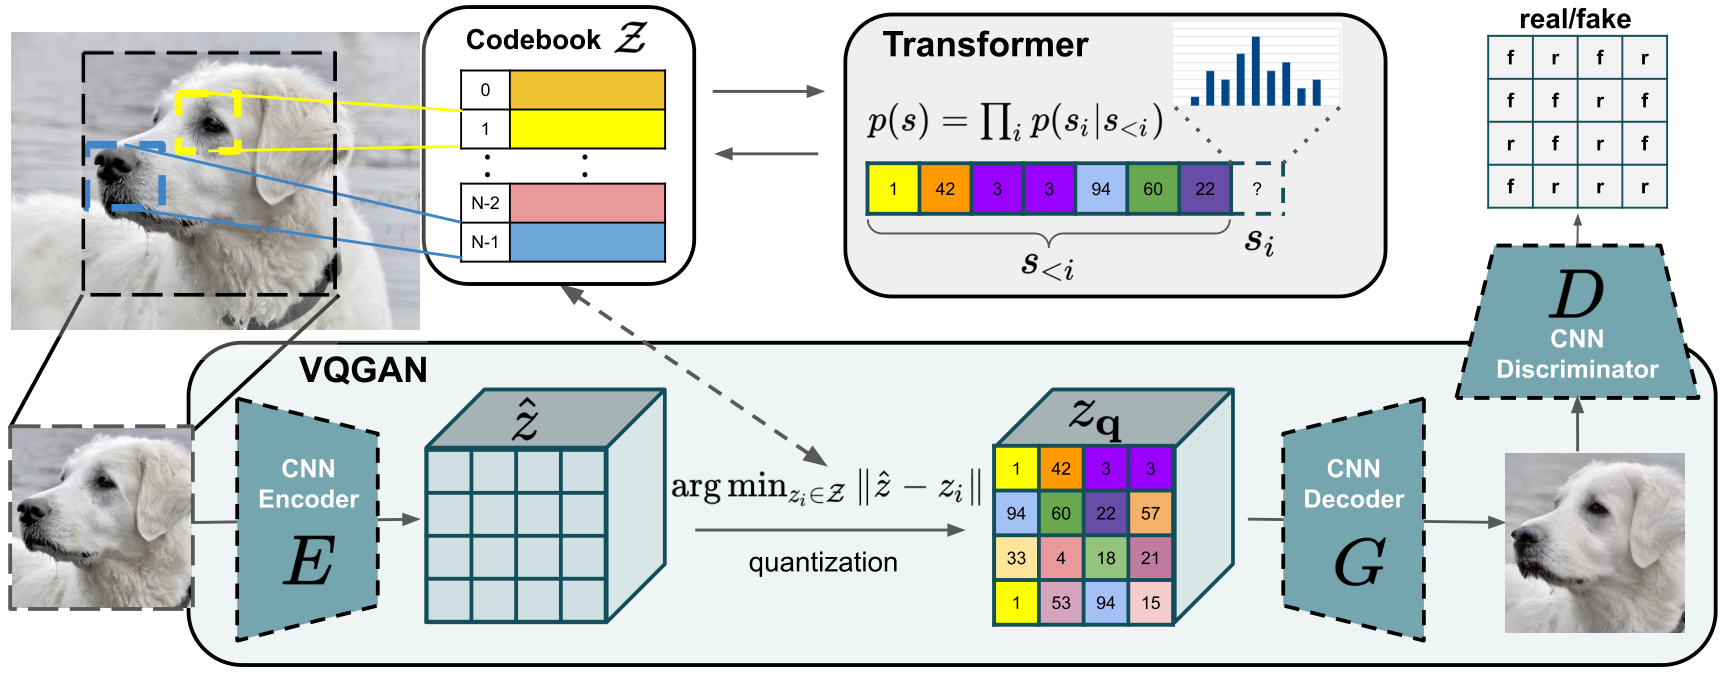
\includegraphics[width=0.9\linewidth]{concept_engineering/vqgan/vqgan.png}
    \caption{VQGAN visualization.\cite{Esser_2021_CVPR}. }
    \label{fig:vqgan-diagram}
\end{figure}

VQGAN has also a transformer part, which is trained to learn connections between embeeding vectors. It is useful for generating images from text.
\paragraph{Loss function}\mbox{}\\

The loss function for VQGAN combines VQVAE and GAN losses:

\begin{itemize}
    \item \textbf{VQVAE loss}: \sout{Reconstruction}, Commitment and Codebook losses,
    \item \textbf{Adversarial Loss}: the GAN component introduces a discriminator that tries to distinguish between real and synthetic images, pushing the generator to create more realistic images,
    \item \textbf{Perceptual similarity loss} instead of Reconstruction loss: ensures the generated image matches the real image in terms of higher-level features, most commonly LPIPS\footnote{\url{https://github.com/richzhang/PerceptualSimilarity}} is used for this puprpose.
\end{itemize}


The optimal compression target $Q^{\star}$ is expressed by the VQVAE loss\eqref{loss_vq} and the GAN loss\eqref{loss_gan} combined together in the formula
\begin{equation}
    Q^{\star} = \text{arg min}_{E,G,Z} \text{max}_D \mathbb{E}_{x~p(x)} [\underbrace{L_{VQ}(E, G, Z)}_{\text{VQVAE loss}} + \lambda\underbrace{L_{GAN}(N, D)}_{\text{adversarial loss}}],
\end{equation}

where $\lambda$ is the scaling factor. It is important to note that reconstruction loss from the $L_{VQ}$ formula\eqref{loss_vq} - $||x-\hat{x}||^2_2$ is calculated as perceptual loss using LPIPS, not the L2 formula. 
% \begin{equation}
%     \mathcal{L}_{GAN}(N,D) = [\log D(x) + log(1-D(\hat{x}))]
% \end{equation}

% \paragraph{Training}\\
% VQGAN should be traon prostate CT scans, learning both a structured latent space and adversarial components to ensure realism.


\paragraph{Generation of CT scans}\mbox{}\\
\indent Generation of CT scans has the same procedure as VQVAE. Firstly LDM is trained and then output is passed through codebook, then decoder. 

% Train it on real CT scans
% To make a new scan, give it some random input
% It will use its codebook and GAN parts to make a realistic-looking CT scan
% % Loss function: VQGAN's loss has several components.

% To generate an artificial CT scan, train the VQGAN on prostate CT scans. This ensures realism.
% To generate a new scan, sample latent codes from the codebook and pass them through the GAN generator.

% To generate a new scan, sample discrete latent codes from the codebook and pass them through the GAN generator.
% The adversarial process refines the image to produce highly realistic synthetic CT scans with well-captured anatomical details.

% \subsection{Stable Diffusion}
\subsubsection{Transfer learning} 
Transfer learning is a popular choice when there is a need to use general purpose model for a specific area. In such case weights of a previously trained neural network are used as a basis for a new neural network model. 
It does not necessairly mean that domain of the new model has to be a subset of the base one. We can assume that base model could learn .
{ImageNet}
\paragraph{}
\subsection{Proposed data generation deep learning algorithms}
\paragraph{DDPM}

\newpage
\subsection{Possible evaluation solutions}
\subsubsection{Algorithms}
Evaluating the quality of artificial model reconstructions or generations necessitates specialized algorithms. These algorithms must be capable of comparing not only individual pixels, but also the structure and semantics of the images.
\paragraph{L1 norm}\mbox{}\\
\indent The L1 norm is also known as the Manhattan distance or the Taxicab norm and is the most straightforward method to measure the distance between vectors, matrices, or tensors. Calculated as the sum of the absolute differences between their components. 
For vectors, the L1 Norm represents the magnitude in a given space. 
In the case of grey CT scan (1,W,H,D) it is calculated as follows:
\begin{equation}
||x-\hat{x}||_1 = \sum_{i=1}^{W} \sum_{j=1}^{H} \sum_{k=1}^{D} |x_{i,j,k}-\hat{x}_{i,j,k}|
\label{norm-l1}
\end{equation}

\paragraph{L2 norm}\mbox{}\\
\indent L2 norm emphasizes larger deviations, making it sensitive to noise and outliers.
\begin{equation}
||x-\hat{x}||_2 = \sqrt{\sum_{i=1}^{W} \sum_{j=1}^{H} \sum_{k=1}^{D} {(x_{i,j,k}-\hat{x}_{i,j,k})^2}}
\label{norm-l2}
\end{equation}
L1 and L2 norms measure pixel-wise differences between generated and real images.
\paragraph{SSIM - Structural Similarity Metric}\mbox{}\\
\indent SSIM is a metric designed to assess image quality by comparing the structural information between two images. Unlike pixel-wise metrics like L1 or L2, SSIM focuses on perceived changes in structural information, such as luminance, contrast, and spatial correlations, which are crucial for medical images like CT scans.
\begin{equation}
    \hbox{SSIM}(x,y) = \frac{(2\mu_x\mu_y + c_1)(2\sigma_{xy} + c_2)}{(\mu_x^2 + \mu_y^2 + c_1)(\sigma_x^2 + \sigma_y^2 + c_2)}
\end{equation}

\begin{itemize}
    \item $\mu_{x}$ - the pixel sample mean of $x$;  
    \item $\mu_{\hat{x}}$ - the pixel sample mean of $\hat{x}$;  
    \item $\sigma_{x}^{2}$ the variance of $x$;  
    \item $\sigma_{\hat{x}}^{2}$ the variance of $\hat{x}$;  
    \item $\sigma_{x\hat{x}}$ the covariance of $x$ and $\hat{x}$;  
\end{itemize}

\begin{equation}
c_{1} = (k_{1}L)^{2}, \quad c_{2} = (k_{2}L)^{2}
\end{equation}
are two variables to stabilize the division with weak denominator.

Where:
\begin{equation}
L = 2^{\#\text{bits per pixel}} - 1,
\end{equation}
$k_{1} = 0.01$ and $k_{2} = 0.03$ by default.

\paragraph{LPIPS - Learned Perceptual Image Patch Similarity}\mbox{}\\
\indent The objective of LPIPS is to assess the perceptual similarity between two images by utilising deep neural networks that have been trained on human visual preferences.

\paragraph{FID - Frechet Image Distance}\mbox{}\\
\indent The FID score compares the distribution of two datasets (real and generated) by calculating the Fréchet distance between multivariate Gaussian distributions, estimated from feature vectors extracted from a pre-trained deep network. The lower the FID score, the more similar the generated images are to the real ones. FVD - Frechet Video Distance.

\subsubsection{Human evaluation}
The final quality of the generated scans or reconstructions can be evaluated by humans. Especially when it comes to assesing the final quality of generated dataset - specialists from the field of radiology and medicine should be the ones to judge whether synthetic dataset has sufficient quality. 

\newpage
\section{Detailed engineering}
\subsection{Programming setup}
Data augmentation using deep learing is a highly complicated process, so choosing the right tooling plays a crucial role in it. Lack of knowledge about modern technologies that help with programming environment setup may lead to many hours of additional time spent on the project that are not specifically related to the core analysis. In order to reduce the time spent on configuration errors, modern state-of-the-art technologies were employed to mitigate this issue.  

\paragraph{Git}\mbox{}\\
\indent Git is a software code versioning system created in 2005. It allows the user to have a local copy of the project code and propose changes to the main copy stored on the remote server, such as Github. Thanks to this tool, collaboration between different programmers is possible. Additionally, unsuccessful attempts or flaws in the implementation may be reverted to the original state.
\paragraph{Github}\mbox{}\\
\indent Enables the user to store git repository on the remote server. The project code is stored in the Github repository.
\paragraph{Data Science project structure}\mbox{}\\
\indent Data Science projects like this often take different forms. Lack of standarization - where and what is stored, may lead to decrease of programmers' productivity over time. Data Science cookie-cutter authors came in the front of this issue. They created a standardized Data Science project structure that can be used to implement a variety of Machine Learning models. 
It has the following form:

\lstinputlisting[basicstyle=\ttfamily\tiny]{detailed_engineering/folder_structure.txt}


The existing project was inspired by the template.
\paragraph{VSCode Remote SSH}\mbox{}\\
\indent Working on a remote computer can be a difficult task to handle. Remote environments often lack the tools that make a programmer effective. Especially a code editor and extensions that the programmer is used to work with and which make a programmer effective in writing code and detecting bugs. VSCode Remote SSH enables a programmer that uses Visual Studio Code to connect to a remote machine with the current editor, so it is almost indistinguishable from the experience of working on a local machine. This way no time was spent on remote code editor setup and extensions installation and configuration. 

\paragraph{Devbox}\mbox{}\\
\indent Remote computers often have their administrators. Almost always they are only ones who are in the super-users' group called "sudoers" in a Linux environment. It helps them keep the machine secure, but also makes them only persons who are able to install additional software, which is later available for everyone. On the other hand, it raises an issue of additional package installation - like specific Python versions and CLI's (Command Line Interfaces) that are required by a project or make a programmer productive.  
To mitigate this issue, a programmer can install software only for himself. However, with the standard Debian/Ubnutu package installer, "apt", it is hard to employ this strategy since many commands still require sudo access. 

Devbox makes it possible to create an environment per project and specify the exact versions of software that should be installed. It can be integrated with Git and Github to make it possible for other programmers to reproduce execalty the same enviornment on their computers. 

Devbox uses the "Nix" package installer under the hood. It is currently the biggest package manager that exists in the Unix landscape. It allows to install most of the open source software that has been ever created. Unfortunatelly, it uses a language that has been specifically created for it. Devbox make it possible to define programs that should be installed in a json file with a specific structure and pin a specific version of the software. Then it creates a lock file in which exact versions for each platform with hashes of the programs are stored. It makes it possible to fully recreate the programming environment created on one computer on another.

CLIs, drivers, versions pinned and managed by the nix package manager.
When it comes to programming environment setup, 

\paragraph{Direnv}\mbox{}\\
\indent When it comes to working with programming projects, the programmer has to switch between them. It requires a Python programmer to change the Python environment to the right one that consists of everything that the project requires to run. Direnv automatically activates the right environment when a directory of the project is entered, so the programmer does not have to do it manually and remember about it.

In the project - Devbox environment and Python environment are automatically enabled when a programmer enters the project directory (and has direnv installed).
\paragraph{Python}\mbox{}\\
\indent Numerous programming languages such as Matlab, Julia, and Elixir support the development of deep learning projects. However, Python stands out as the primary language for most research and advancements in Artificial Intelligence. Therefore, it was the natural choice for this project.
\paragraph{Rye}\mbox{}\\
\indent Almost every Python project nowadays uses external libraries written by other programmers. It makes the programmer not reinvent the wheel again and dramatically reduces the project implementation time. However, it raises the issue of external package version management. To tackle this issue, Python programmers came up with the'requirements.txt' file that should include all external, non-standard, dependencies that the project requires in order to make the environment reproducible on the other computer. In addition, they introduced the `pip` package manager that allows them to be installed. 
Rye is a more modern solution to this problem. It enables the user to create a Python package from the existing project, define external dependencies with their exact versions, and create a Python virtual environment. 

What is more - it makes it possible to use a modern replacement for the `pip` package manager - uv. UV is a modern package installer written in Rust that is in some cases even 100 times faster in comparison to its predecessor.  
\paragraph{Pytorch}\mbox{}\\
\indent Pytorch is a Deep Learning framework for Python programmers. It makes it possible to create neural networks and train them on a GPU. It is currently the most widely used framework in the Deep Learining landscape according to... 
Most of the nowadays research on the neural networks is done using this framework, so it was an obvious choice, since the project was meant to use state of the art neural network written by other programmers. Using this framework made it possible to reuse their code without reimplementation. 
\paragraph{Pytorch Lightning}\mbox{}\\
\indent Implementing neural networks in Pytorch always consists of some repetitive steps, such as recording, training callbacks, retraining, using multiple gpus. Pytorch Lightning authors noticed this issue and created a standard template for Deep Learning model training that proposes a standard structure for a model training, which makes code more readable and easier to modify. Additionally, they employ researcher with many tools that make the programmer more effective, like callbacks mechanism, floating point precision switching, and most importantly, multiple GPU training. Without it, it would be necessary to have deep knowledge about multiple-gpu training. With Pytorch Lightning multiple gpu training was possible with only one parameter switch. 

Deep Learning framework that utilizes Pytorch. 
\paragraph{Monai}\mbox{}\\
\indent Deep Learning framework for medical purposes.
\paragraph{Nohup}\mbox{}\\
\indent CLI that keeps the process running even after the user's log-out/session ends.
\newpage
\subsection{Hardware}
Training neural networks demands substantial computational resources, particularly for the latest architecture models. These models typically consume significant memory, making it impractical to train them on personal computers. To address this, two Nvidia Quadro RTX 8000 GPUs, each equipped with 48GB of RAM, were utilized. 

\subsection{Hardware utilisation - Multiple GPU utilisation techniques}
Training on a single GPU is straightforward. However, when a single card falls short, the challenge of leveraging multiple GPUs arises. The solution varies based on the underlying reason for employing multiple GPUs.
\paragraph{Distributed data parallel}\mbox{} \\
If a single GPU can handle training a neural network but you wish to speed up the process with an additional GPU, the Distributed Data Parallel (DDP) technique can be used. This approach distributes the neural network model and data across both GPUs, allowing for concurrent training of two model instances. However, during the backpropagation phase, the gradients are synchronized and averaged.

This technique was used to train most of the models presented later, since it sped up the training twice. 

\paragraph{Distributed data parallel sharded}\mbox{} \\
If one GPU is unable to fit into its memory model, then the distributed data parallel shared technique can be used to solve the issue. Splits the model layers between cards and then uses cross-device communication techniques to train the model. However, this solution slows down the training due to the overhead of cross-device communication.

\newpage 
\subsection{Training monitoring}
Training of neural networks often takes a lot of time - hours, days, weeks and sometime even months. It is crucial to monitor it in order not to waste resources on unsuccessful training. Whats more - when there are many models that are trained or there are many attempts of training it is easy to loose track of what has been accomplished, which models were already trained and what were the results. 
Monitoring enables the researcher to have visibility of important metrics for the model. Thus, unsuccessful training may be stopped ahead of time. It also helps to visualize training progress, model output and makes it possible to share the results with other researchers during the training. 
\paragraph{Tensorboard}
Tensorboard is an open source project that enables user to locally monitor training of a neural networks. It makes it possible to:
- gather metrics,
- visualize model outputs,
- organize model trainings in the friendly user interface.

\paragraph{Wandb}
Wandb is a commercial product that allows to monitor training of Machine Learning models, especially deep learning ones. W skład monitoringu wchodzi:
- gathering statistics and metrics
- comparison of statistics,
- hardware monitoring,
- configuration monitoring. 
- reports of training. 

It can be synchronised with Tensorobard. The metrics logged there can be viewed in the WanDB website. They give researchers from the academia free resources to use. 

Thanks to the tool it was possible to monitor whether model converges or not.

\newpage
\subsection{Dataset}
\paragraph{Data source}
\paragraph{Data format - DICOM}
- NII.GZ
- 
\paragraph{Data characteristics}
- count
- value range
- number of layers
\paragraph{Data transformations}

\newpage
\subsection{Chosen approaches}
% \subsubsection{WGAN}
% \subsubsection{Autoencoder}
\subsubsection{VAE + DDPM}
\input{}
The first attempt to generate artificial scans was based on the variant autoencoder architecture proposed in \cite{rombach2022high}. The implementation was based on the Monai\cite{Cardoso_MONAI_An_open-source_2022} example available on Github\footnote{\url{https://github.com/Project-MONAI/GenerativeModels/blob/e7cc989cdce440a7bff1cce22fff1caf760f39cd/tutorials/generative/3d_autoencoderkl/3d_autoencoderkl_tutorial.ipynb}} and adjusted to Pytorch Lightning.

\begin{figure}[H]
\minipage{0.49\textwidth}
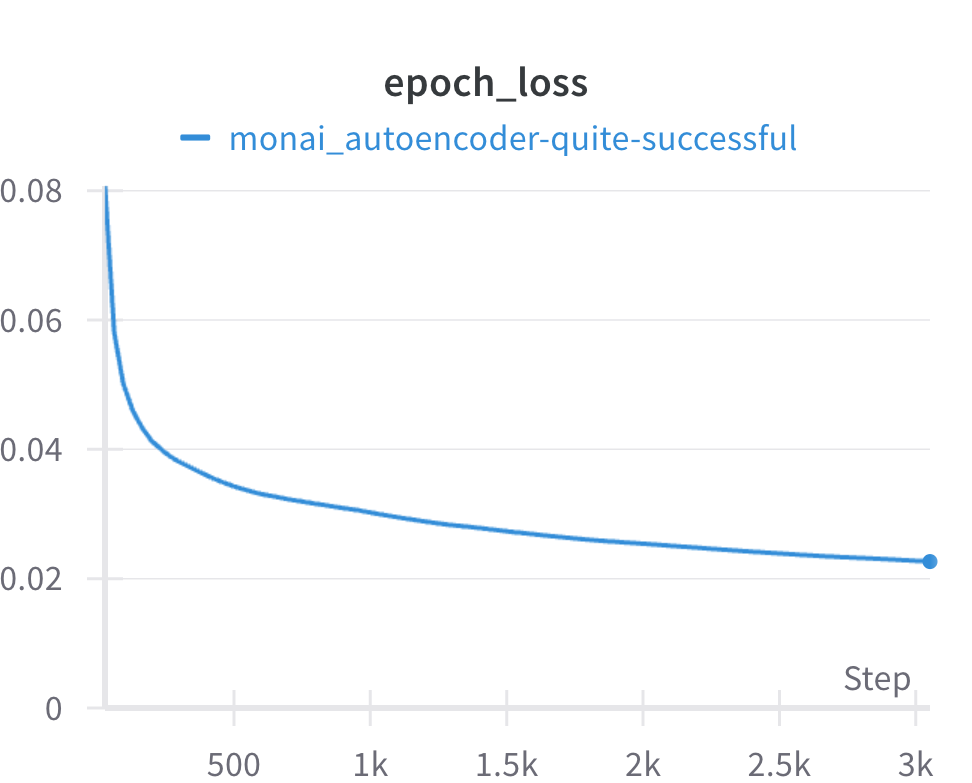
\includegraphics[width=\linewidth]{detailed_engineering/Monai Autoencoder/charts/epoch_loss.png}
\caption{}
\endminipage\hfill
\minipage{0.49\textwidth}
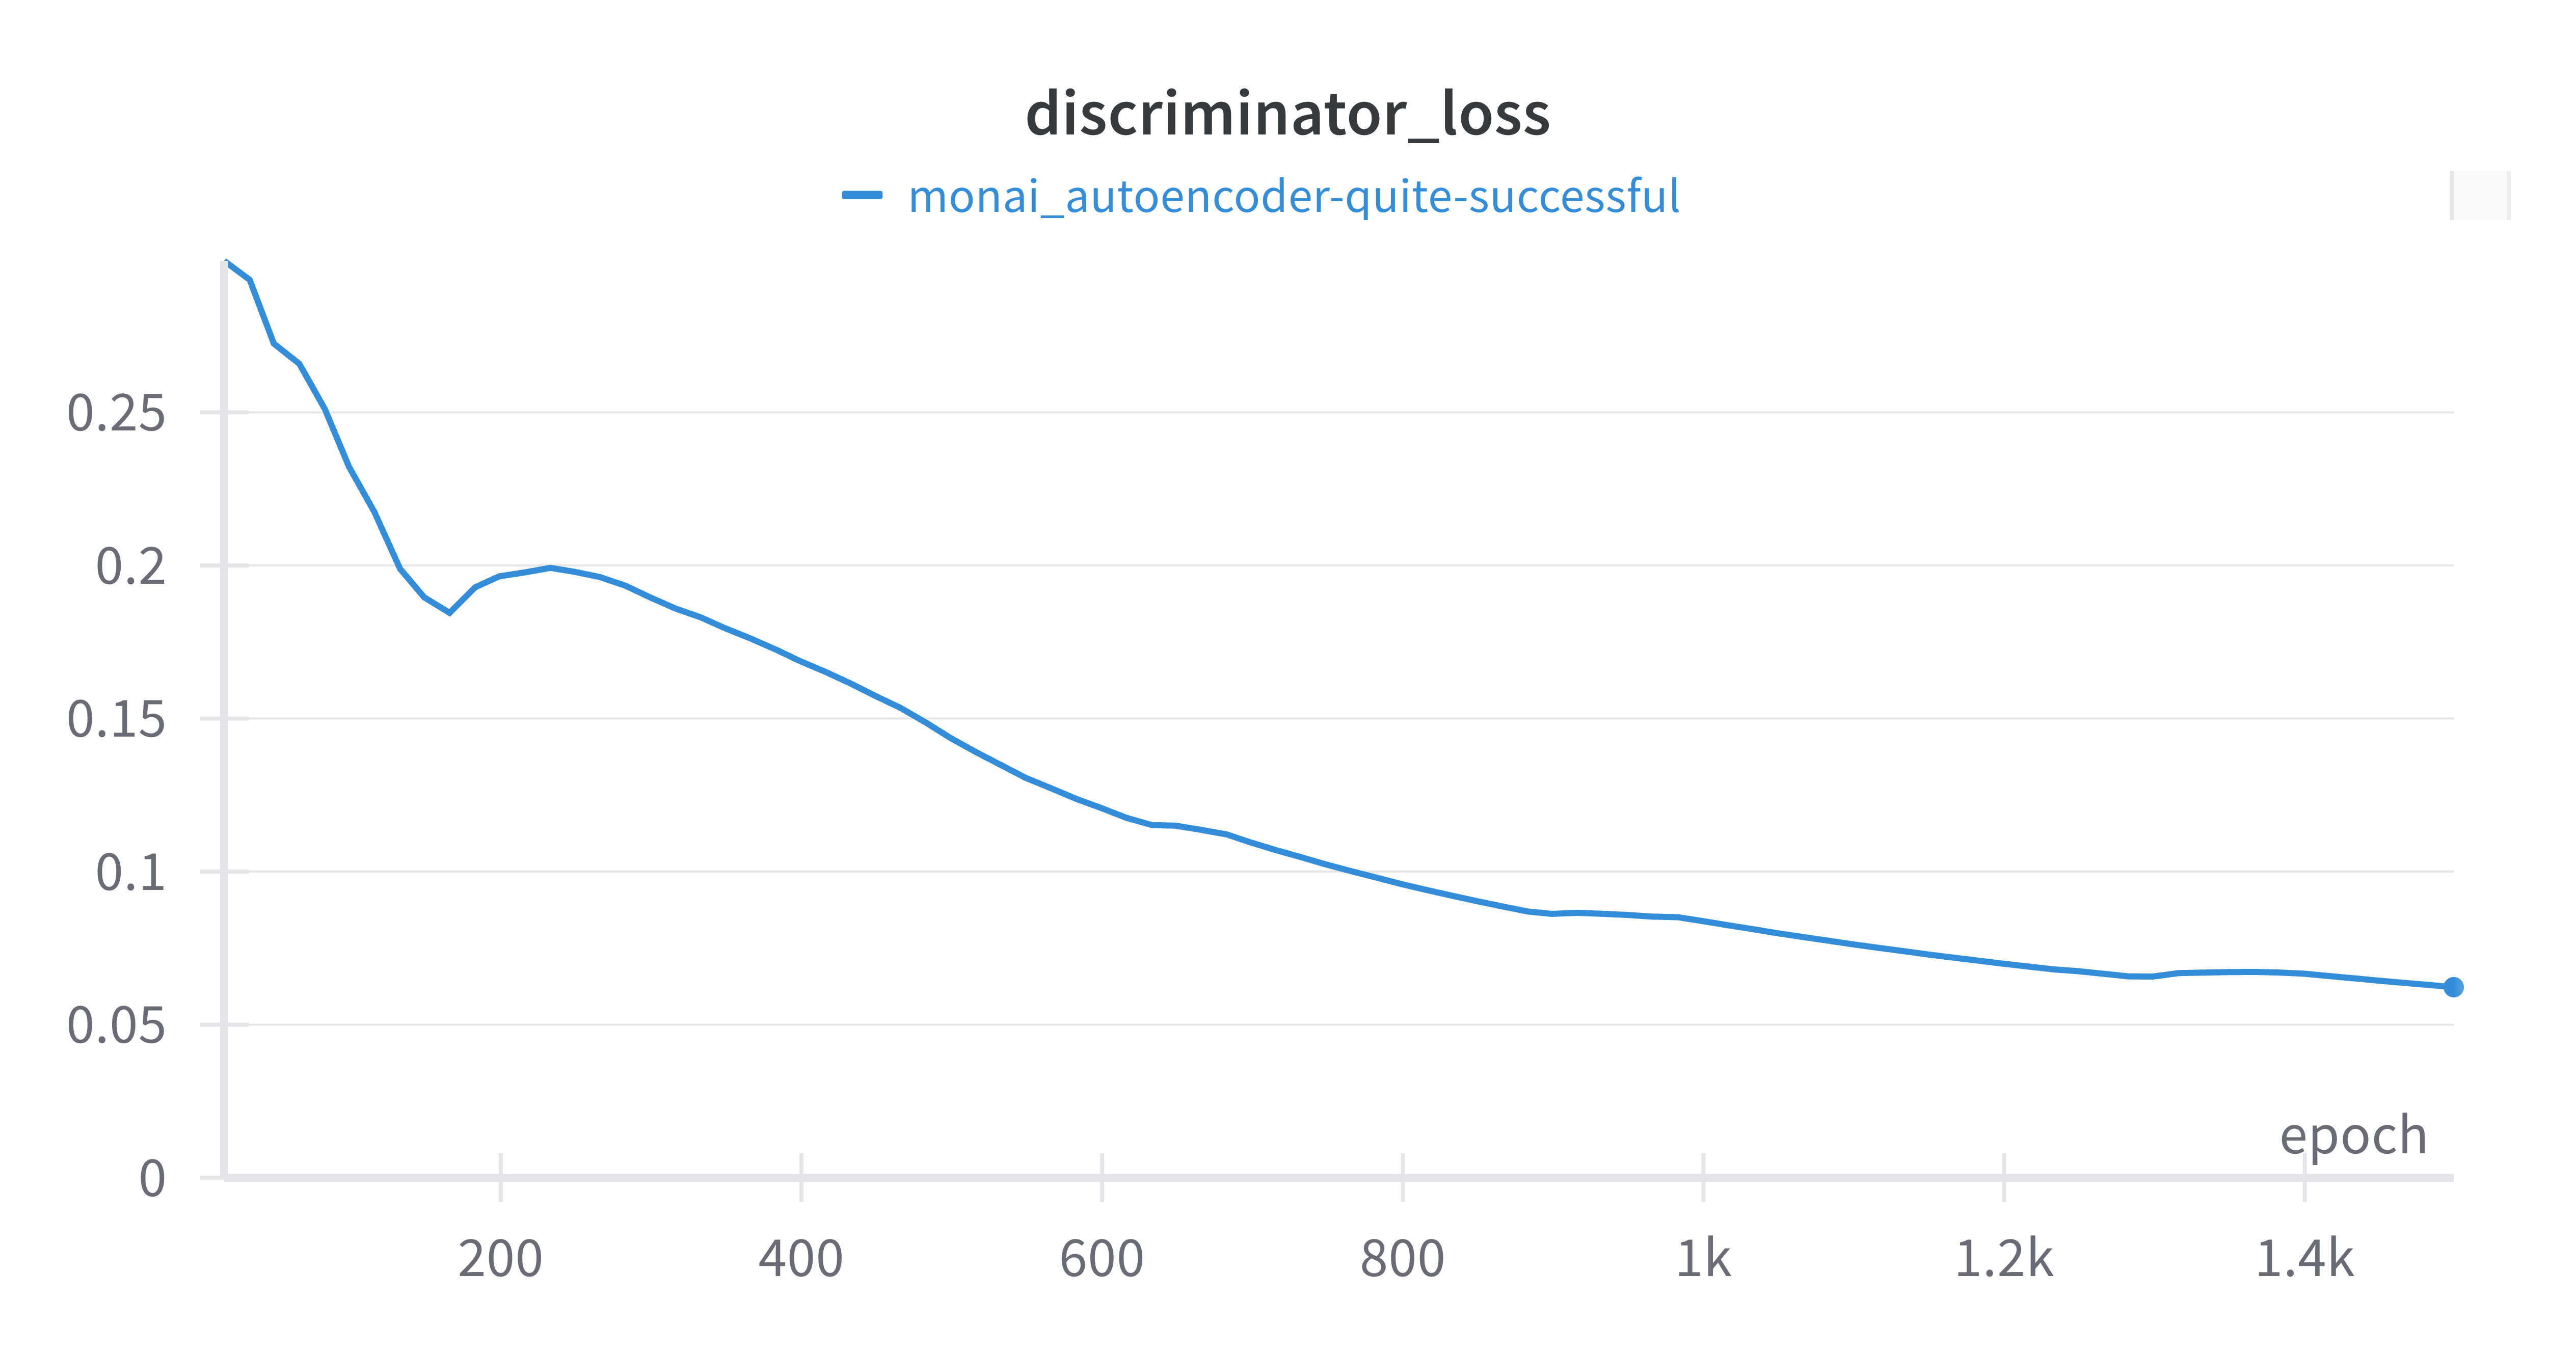
\includegraphics[width=\linewidth]{detailed_engineering/Monai Autoencoder/charts/discriminator_loss.png}
\caption{}
\endminipage
\end{figure}

\begin{figure}[H]
\minipage{0.49\textwidth}
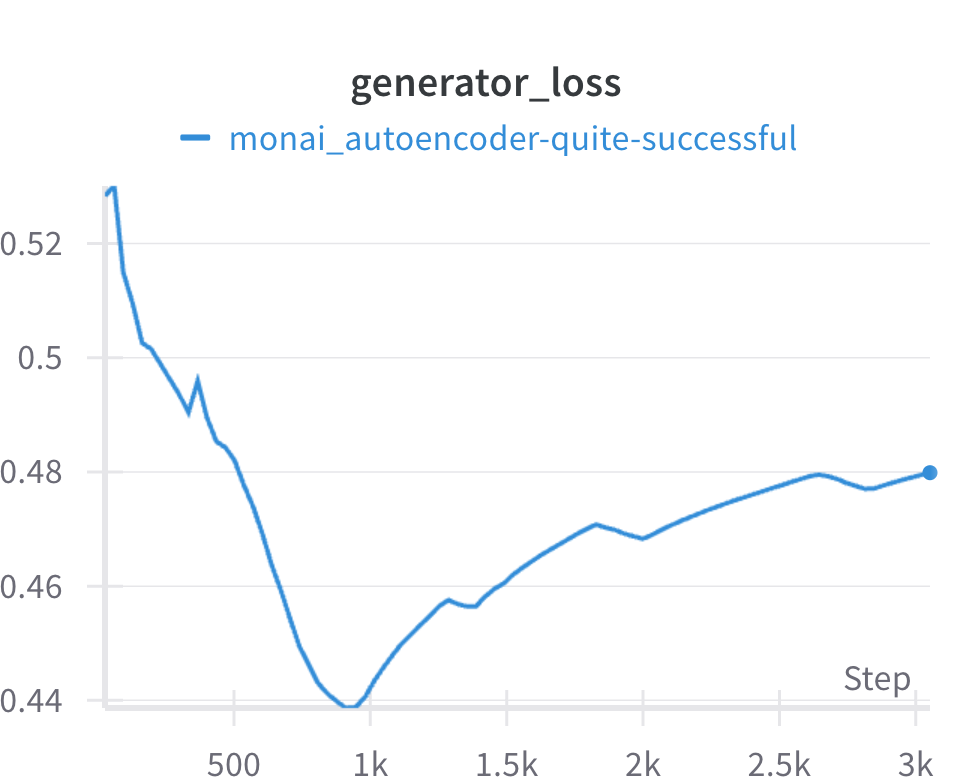
\includegraphics[width=\linewidth]{detailed_engineering/Monai Autoencoder/charts/generator_loss.png}
\caption{}
\endminipage\hfill
\minipage{0.49\textwidth}
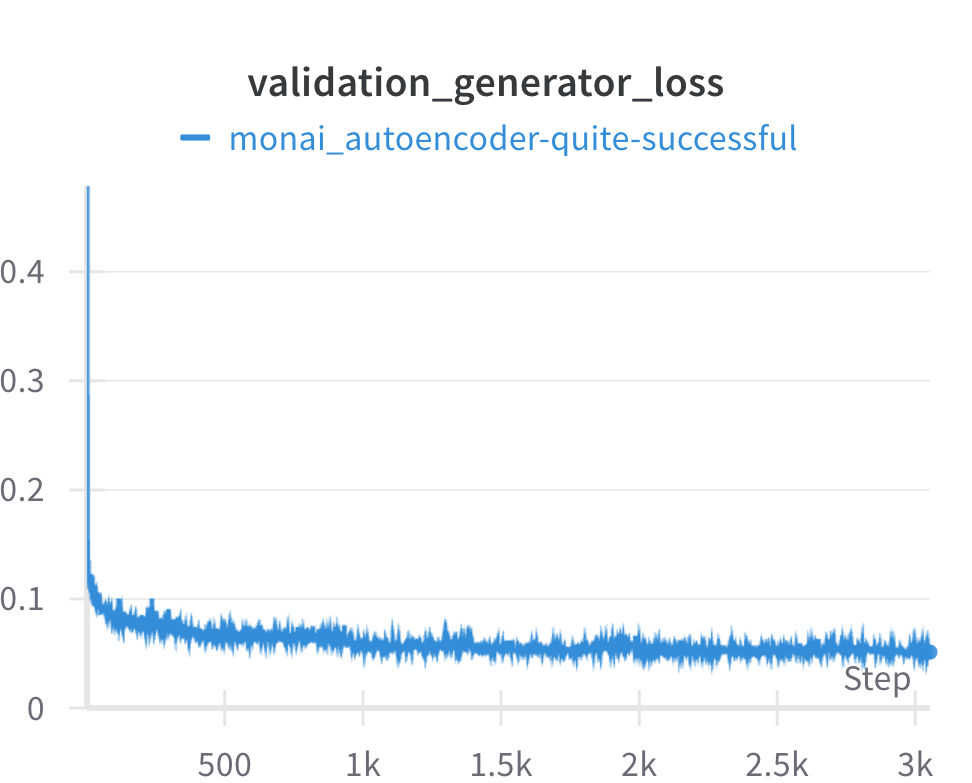
\includegraphics[width=\linewidth]{detailed_engineering/Monai Autoencoder/charts/val_generator_loss.png}
\caption{}
\endminipage
\end{figure}


\begin{figure}[H]
% \minipage{0.49\textwidth}
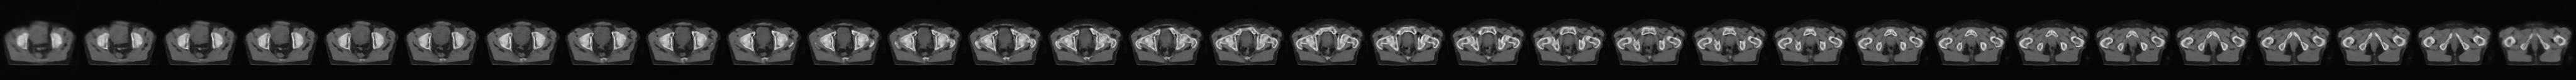
\includegraphics[width=\linewidth]{detailed_engineering/Monai Autoencoder/charts/reconstruction.png}
\caption{}
% \endminipage\hfill
% \minipage{0.49\textwidth}
% \includegraphics[width=\linewidth]{charts/Section-4-Panel-5-z2xepgyu7}
% \caption{}
% \endminipage
\end{figure}
d




\paragraph{LDM Attempt 1}\mbox{}\\

In this attempt $z$ was sampled from $\mathcal{N}(0,1)$ and passed through the decoder. 

\begin{figure}[H]
\minipage{0.49\textwidth}
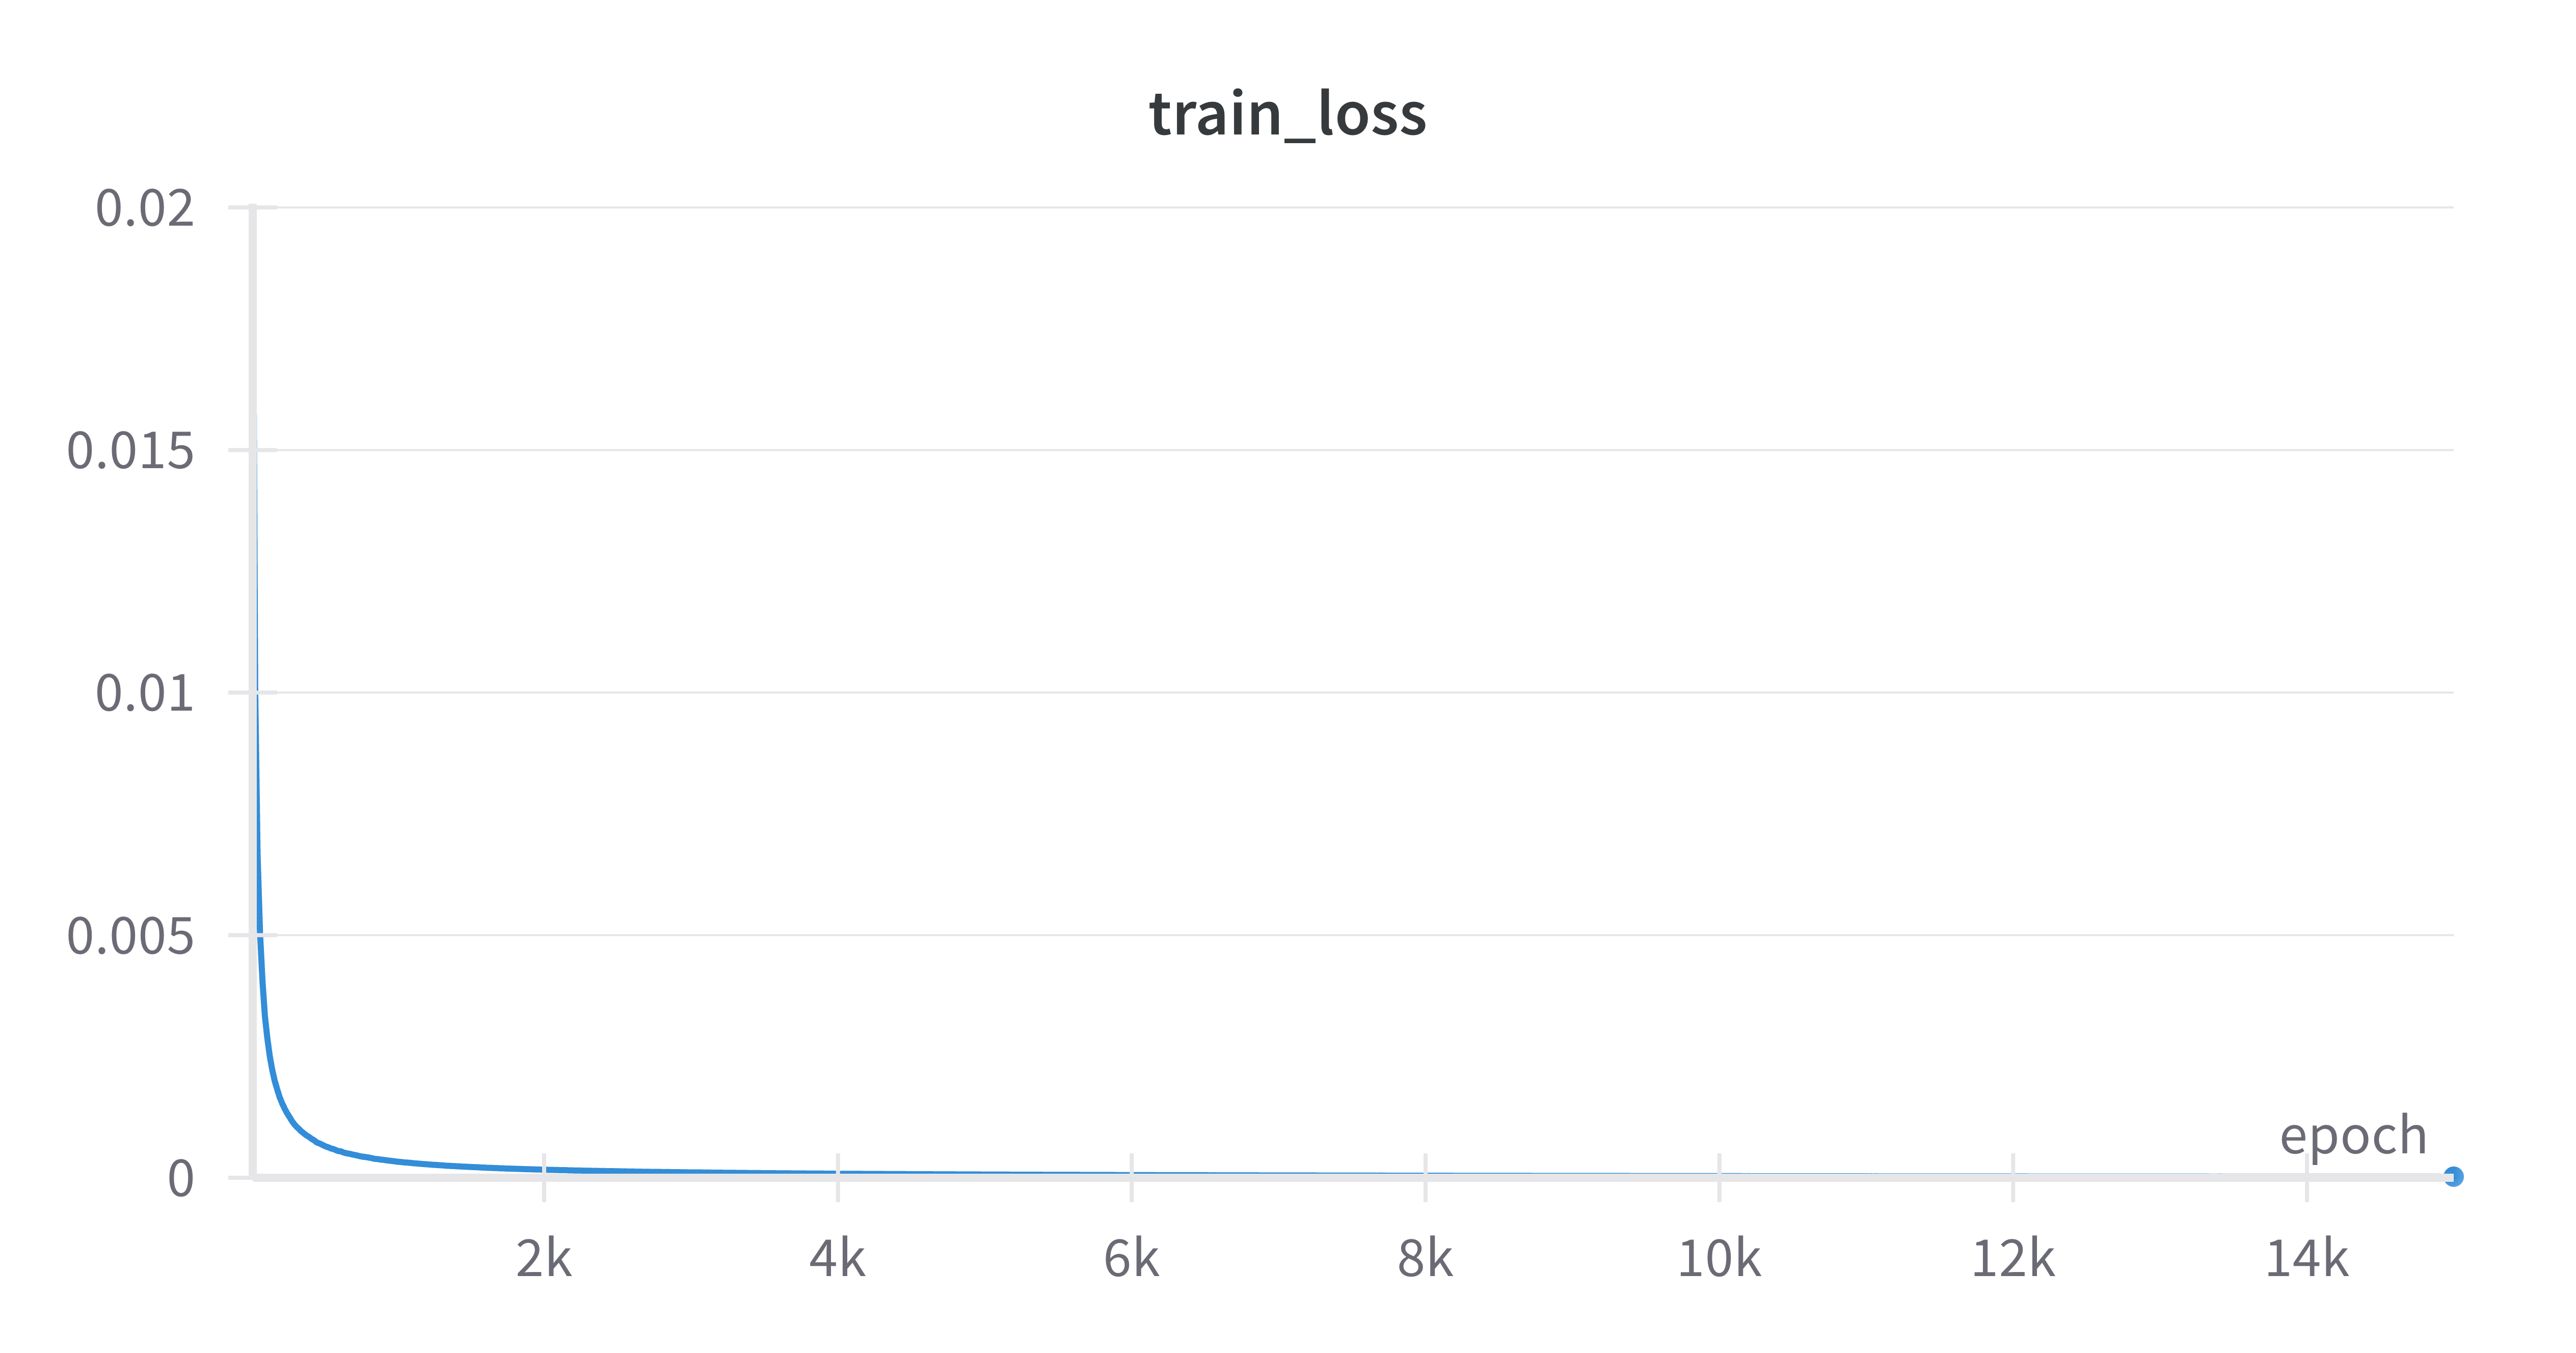
\includegraphics[width=\linewidth]{detailed_engineering/Monai Diffusion - Attempt 1/charts/train_loss.png}
\caption{}
\endminipage\hfill
\minipage{0.49\textwidth}
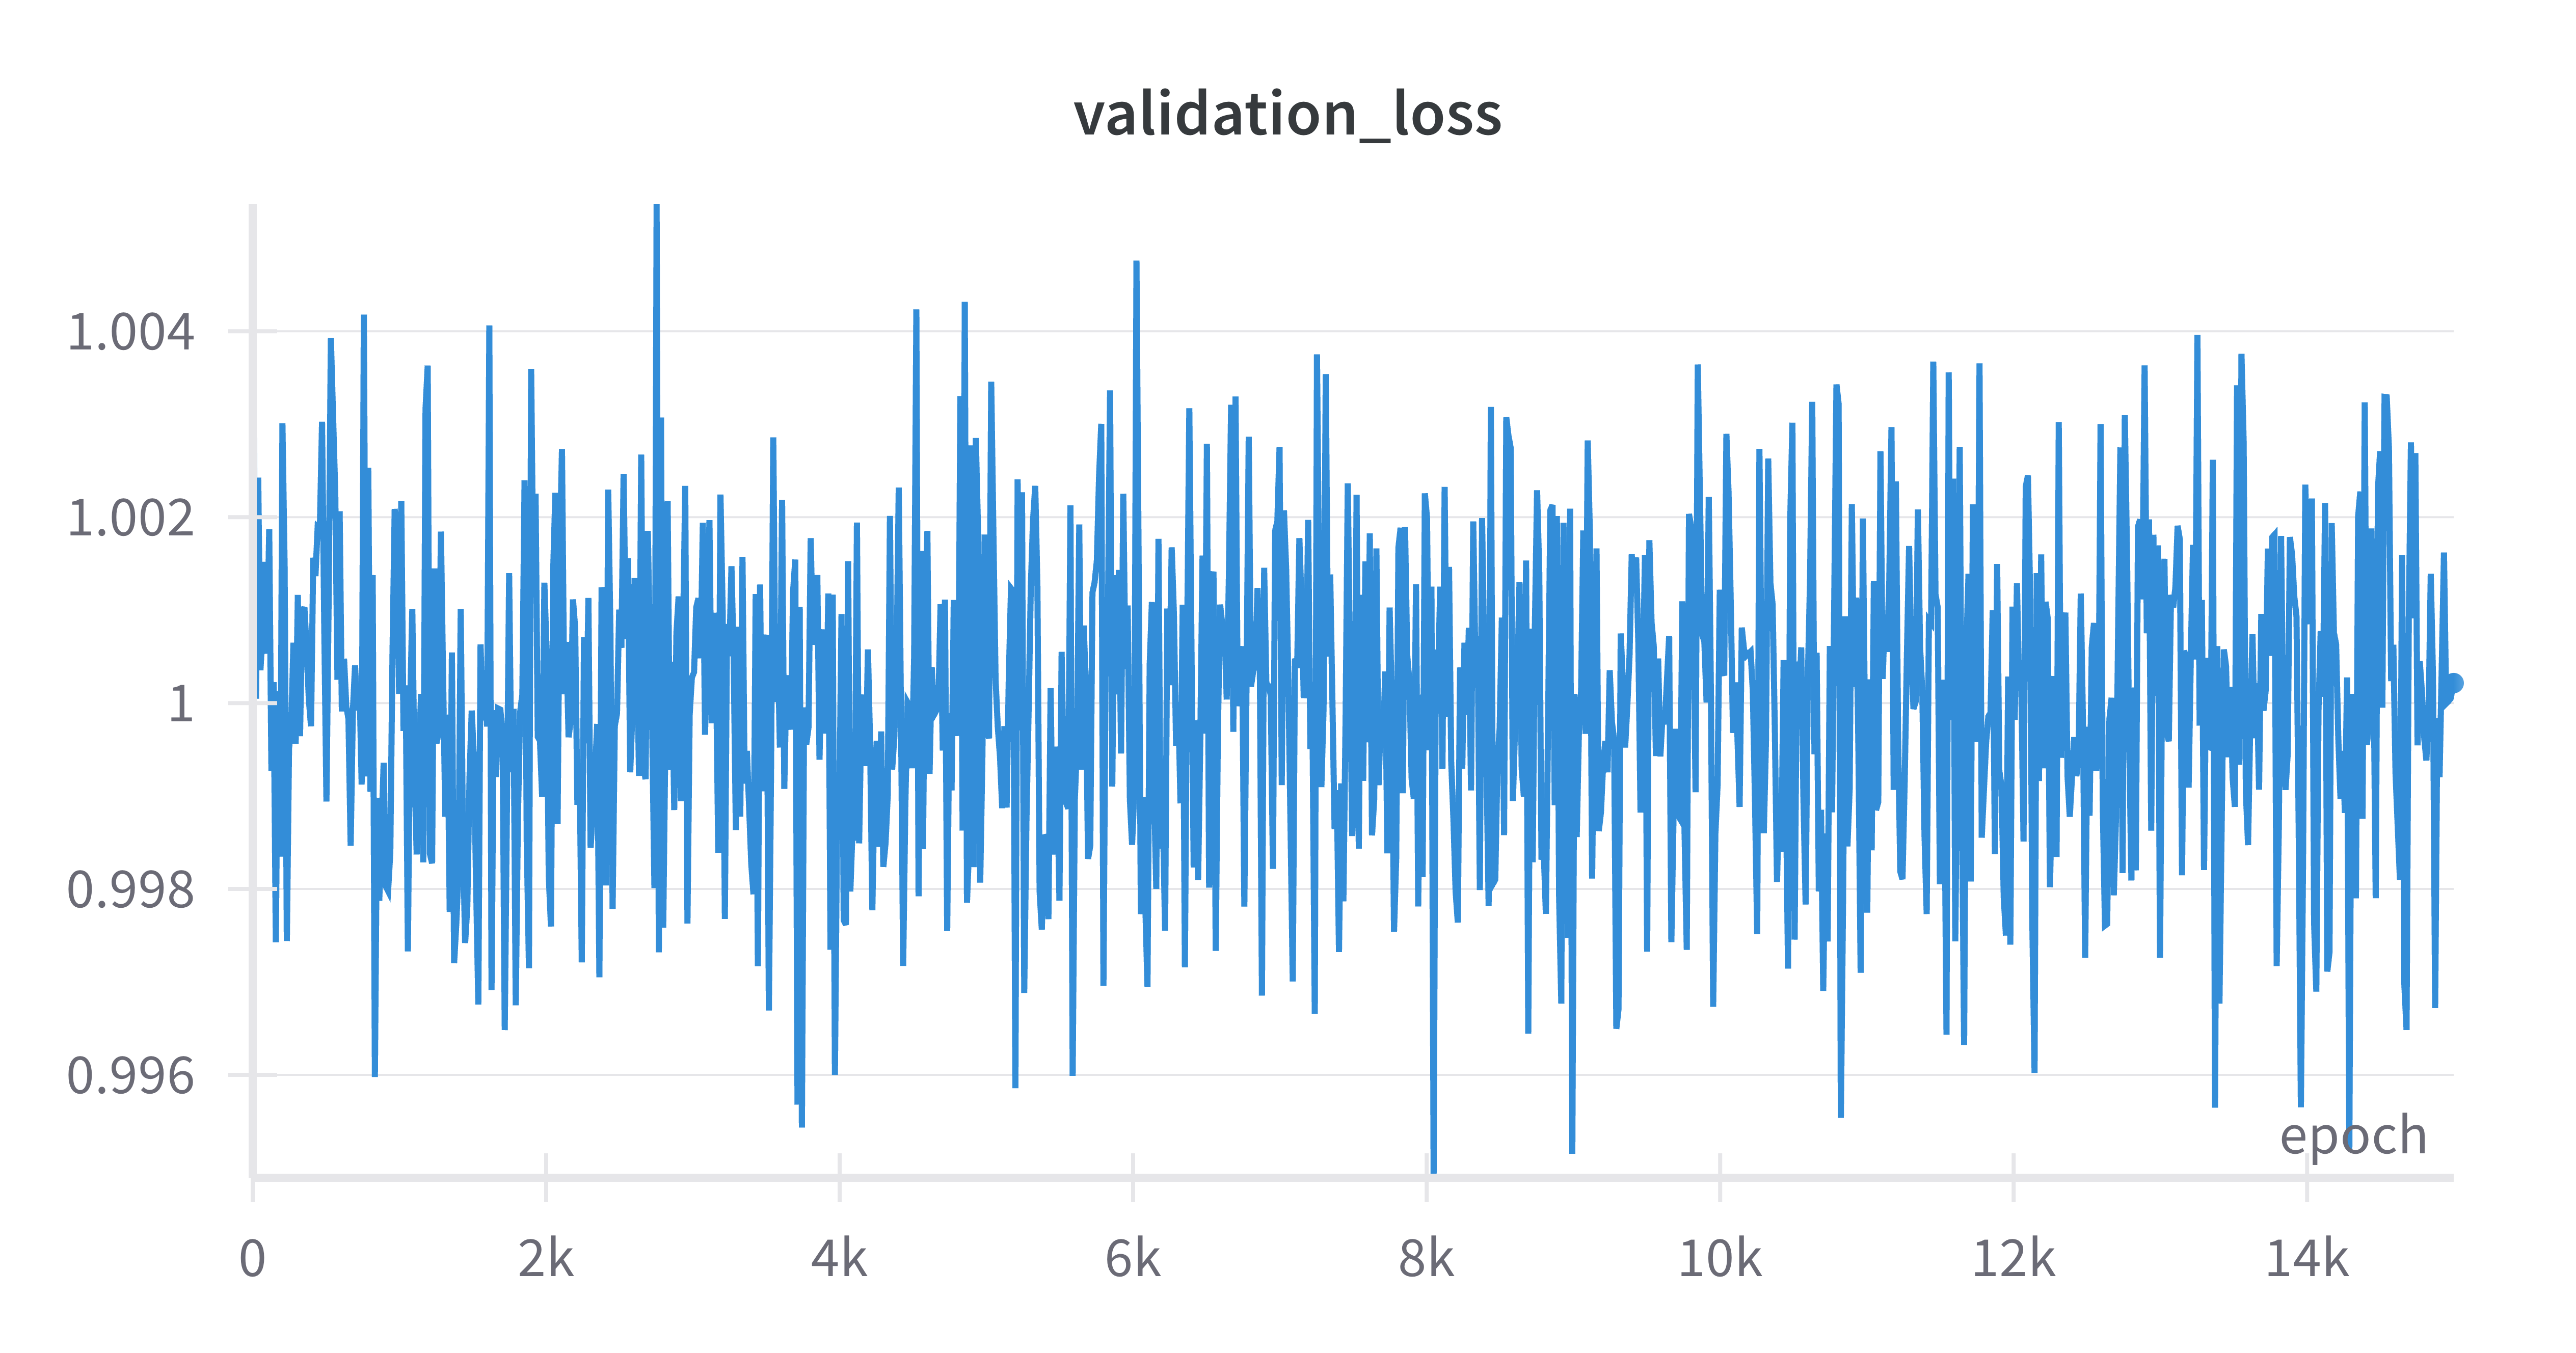
\includegraphics[width=\linewidth]{detailed_engineering/Monai Diffusion - Attempt 1/charts/validation_loss.png}
\caption{}
\label{fig:ldm_a1_val_loss}
\endminipage
\end{figure}


\begin{figure}[H]
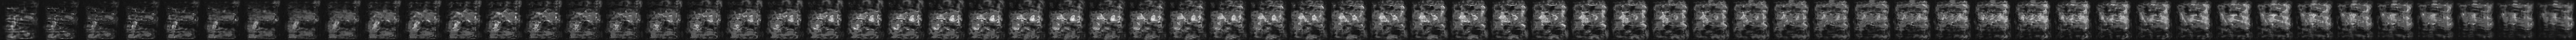
\includegraphics[width=\linewidth]{detailed_engineering/Monai Diffusion - Attempt 1/charts/generation.png}
\caption{Unsuccessful generation of synthetic CT scan.}
\label{fig:attempt1-generation}
\end{figure}

Generation was unsuccessful\ref{fig:attempt1-generation}. The validation loss did not decrease\ref{fig:ldm_a1_val_loss}.


\paragraph{LDM Attempt 2}\mbox{}\\

\indent In this attempt instead of creating noise from $\sim\mathcal{N}(0,1)$, the noise was generated from $N(\mu, \sigma)$ where $\mu$ is the mean of the training data $z_{\mu}$ and $\sigma$ is the mean of $z_{\sigma}$ obtained from the training data set (25 samples).

\paragraph{Model configuration}\mbox{}\\
The configuration was the same as in Attempt 1. The only difference was in the noise generation approach.

\paragraph{Training}\mbox{}\\
\begin{figure}[H]
\minipage{0.49\textwidth}
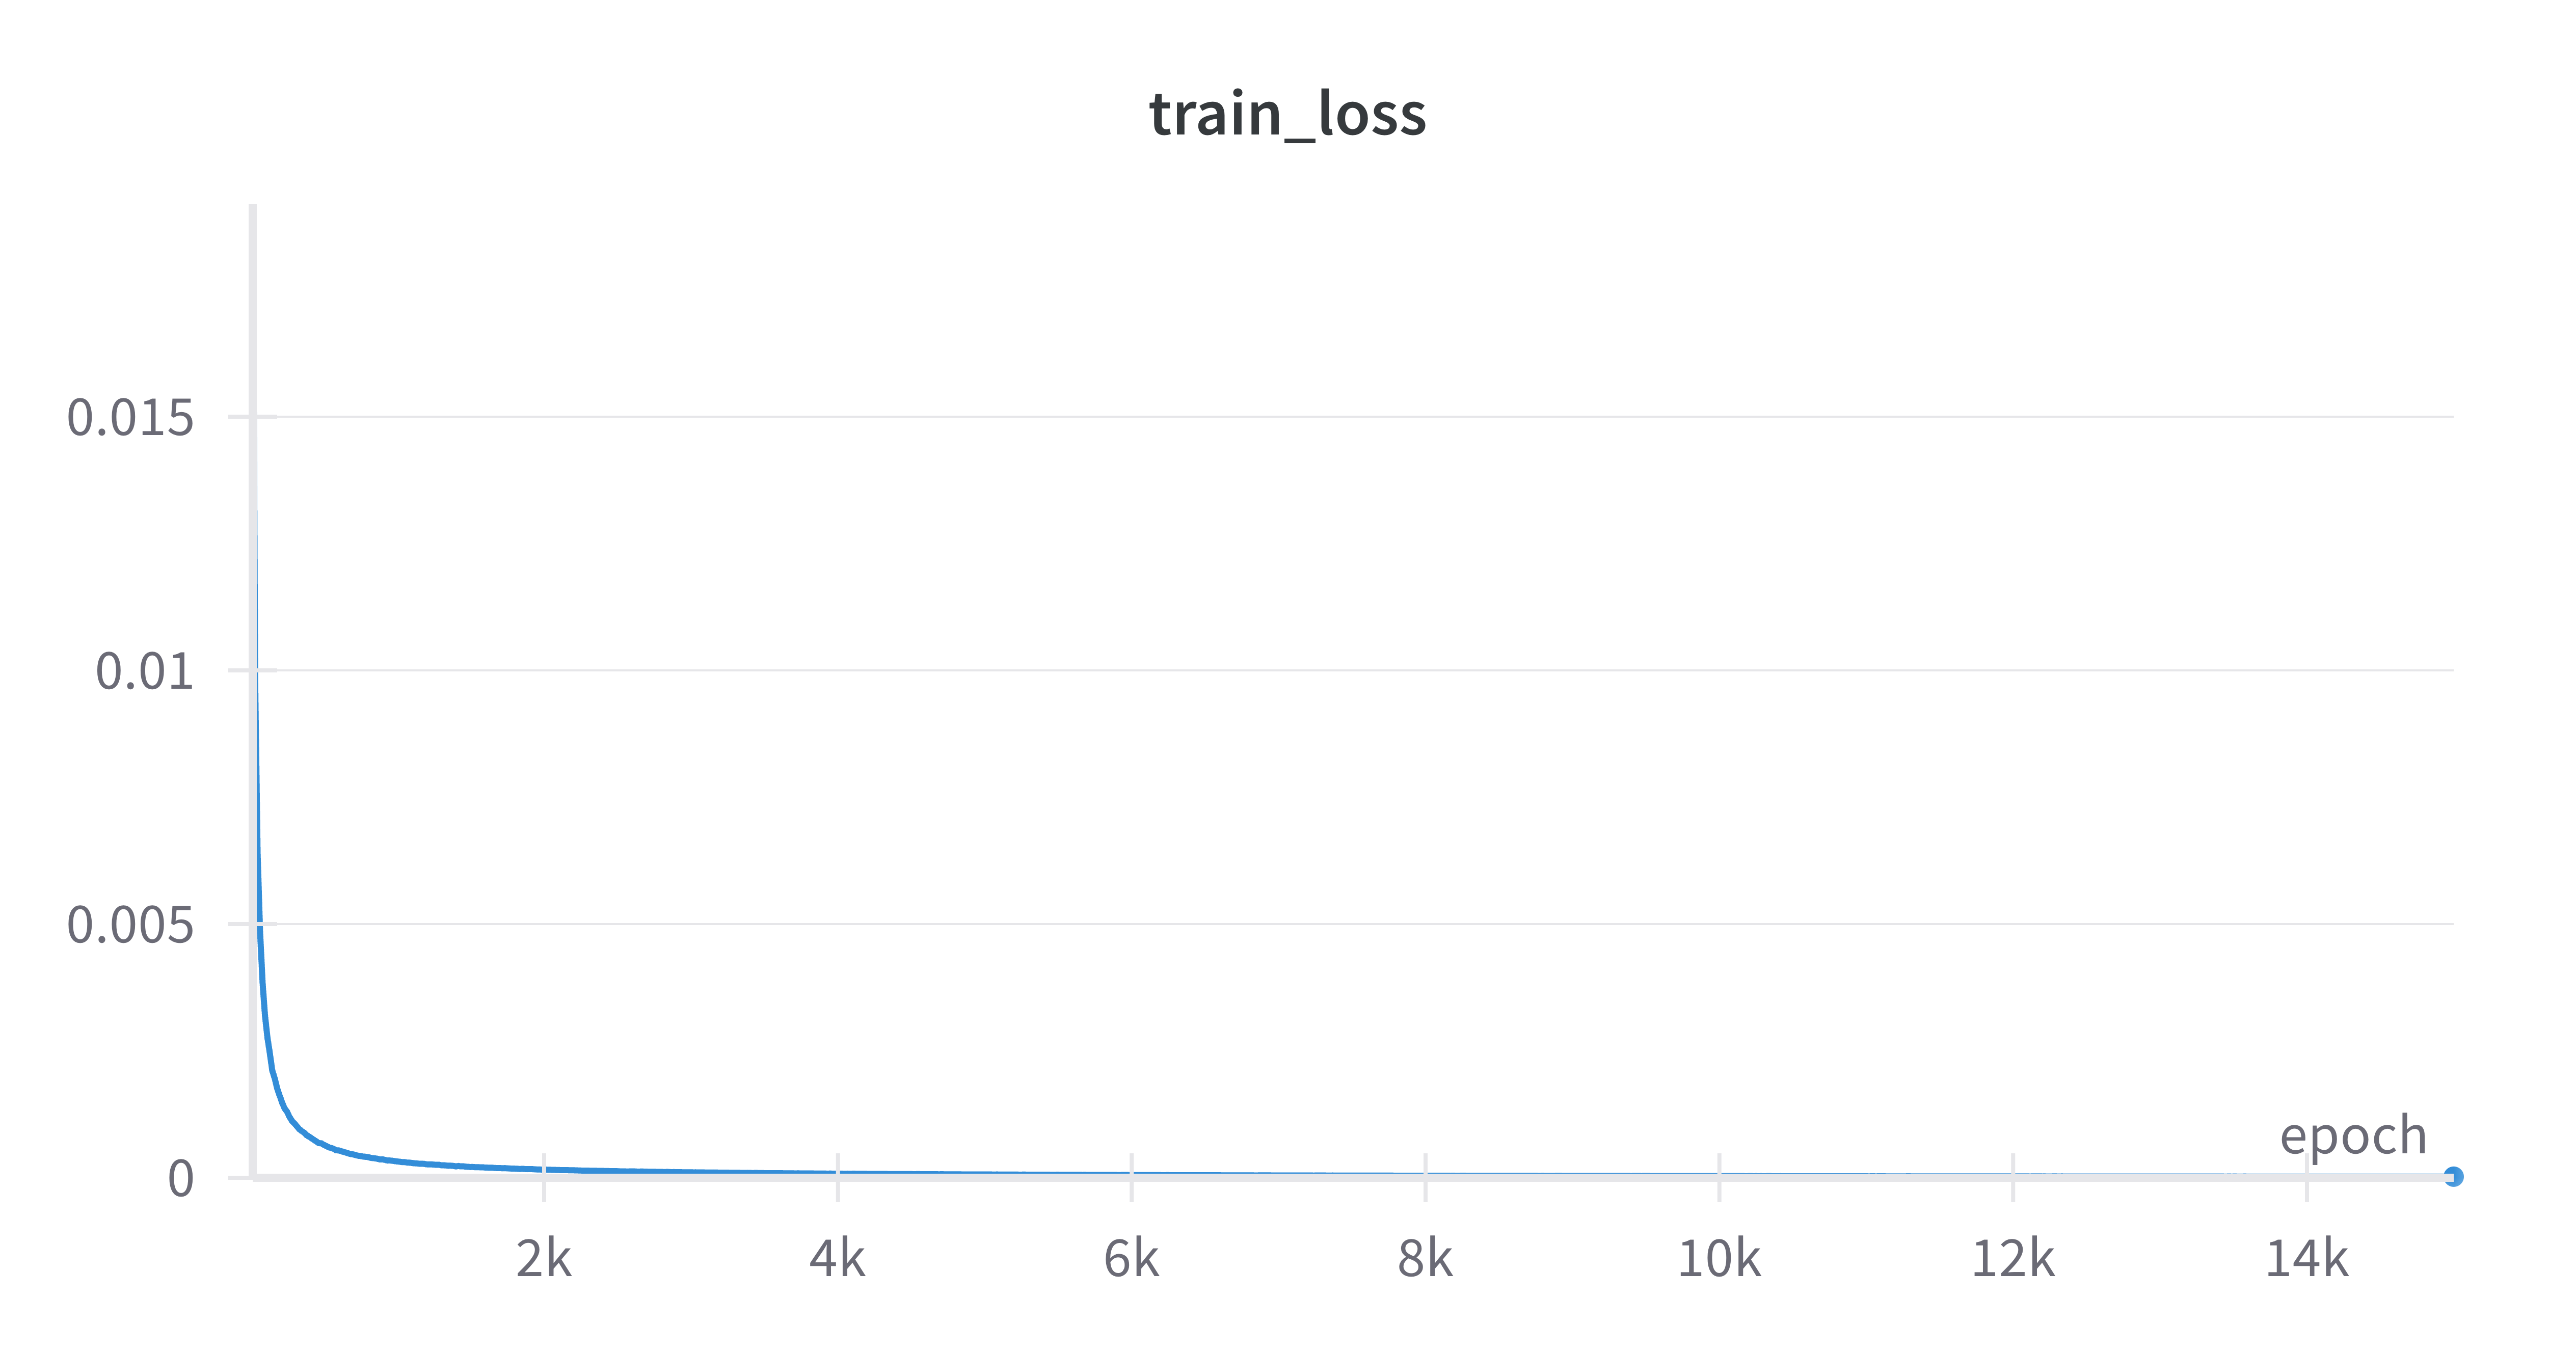
\includegraphics[width=\linewidth]{detailed_engineering/Monai Diffusion - Attempt 2/charts/train_loss.png}
\caption{}
\endminipage\hfill
\minipage{0.49\textwidth}
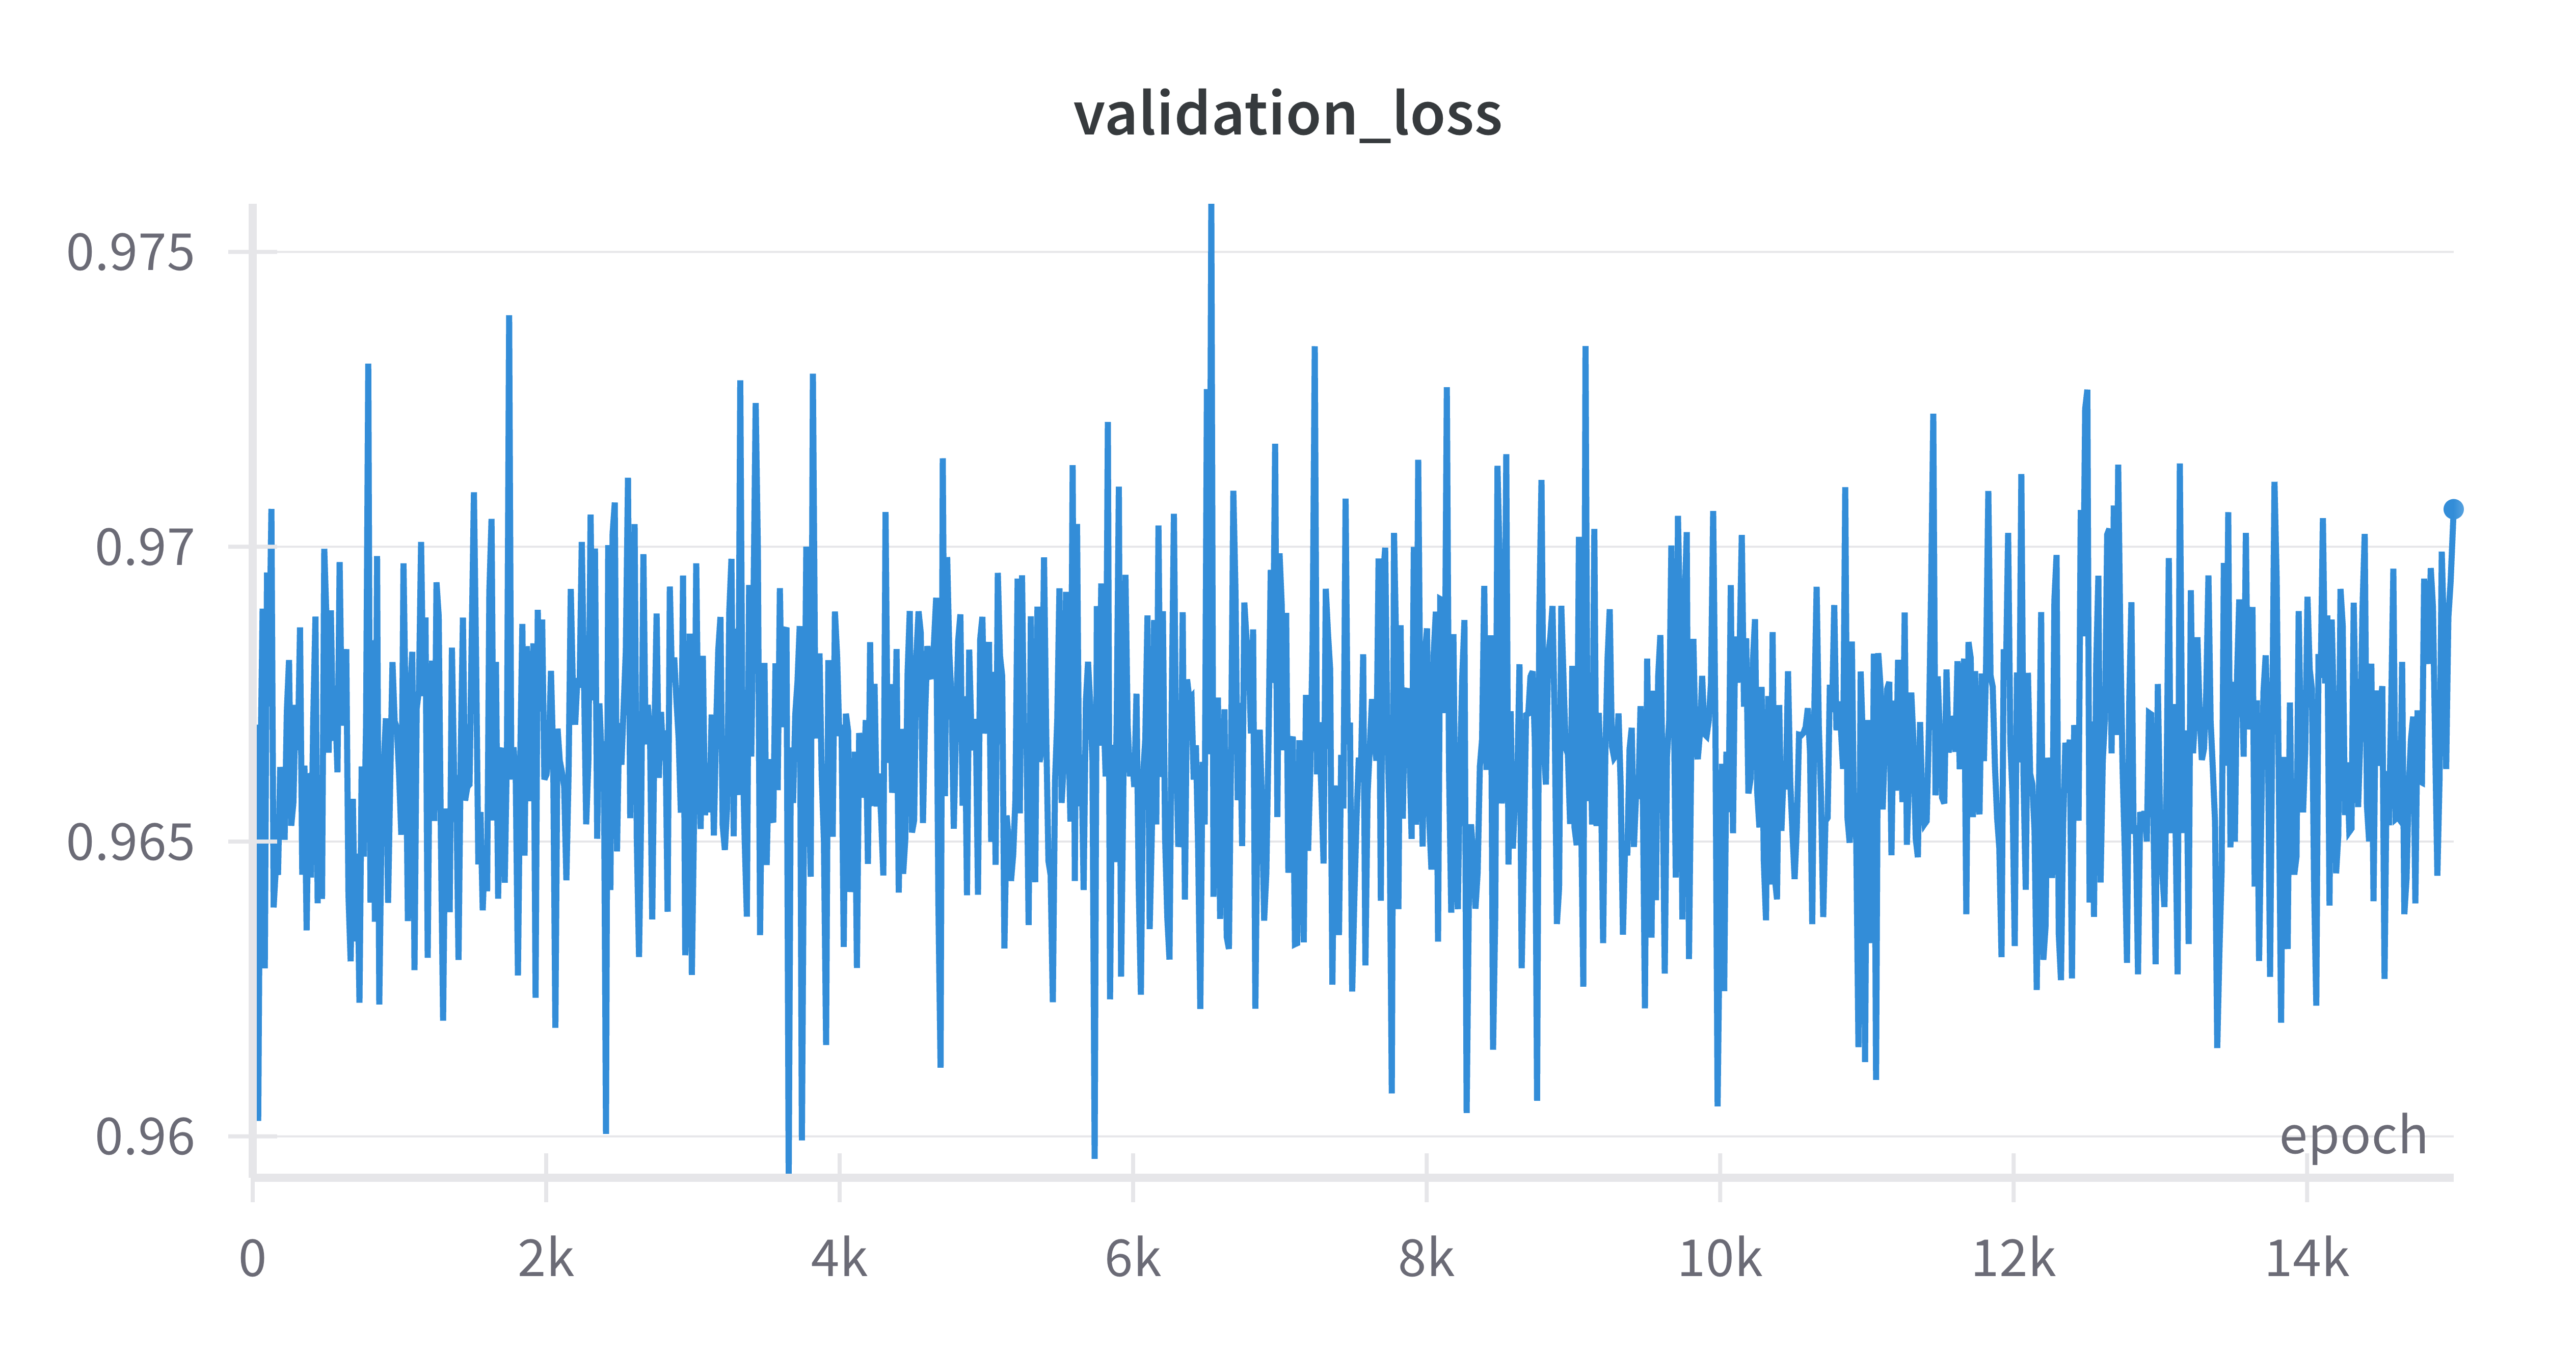
\includegraphics[width=\linewidth]{detailed_engineering/Monai Diffusion - Attempt 2/charts/validation_loss.png}
\caption{}
\label{fig:ldm_a2_val_loss}
\endminipage
\end{figure}

As is visible in the figure \ref{fig:ldm_a2_val_loss}, the validation loss did not decrease. The output of the generation was the same as in the previous attempt.






\newpage
\subsubsection{Transformers CT: VQVAE + Transformers}
The VQVAE\footnote{\url{https://github.com/FirasGit/transformers_ct_reconstruction}} model and its complementation are based on the one presented in article\cite{khader_transformers_2023}.

Due to time constraints, the VQGAN and transformer models presented in the work have not been trained. Only VQVAE was trained and the result of this process is presented below. 


\paragraph{VQVAE}\mbox{}\\
\paragraph{Model configruation}\mbox{}\\

\begin{table}[h!]
\centering
\begin{tabular}{|l|l|}
\hline
\textbf{Parameter} & \textbf{Value} \\
\hline
\multicolumn{2}{|c|}{\textbf{Training}} \\
\hline
Accelerator & GPU \\
\hline
Devices & 2 \\
\hline
Precision & 32 \\
\hline
Strategy & DDP \\
\hline
Maximum Epochs & 10001 \\
\hline
\multicolumn{2}{|c|}{\textbf{Model}} \\
\hline
Input Channels & 1 \\
\hline
Output Channels & 1 \\
\hline
Embedding Channels & 8 \\
\hline
Number of Embeddings & 16384 \\
\hline
Spatial Dimensions & 3 \\
\hline
Hidden Channels & [32, 64, 128, 256] \\
\hline
Kernel Sizes & [3, 3, 3, 3] \\
\hline
Strides & [1, 2, 2, 2] \\
\hline
Embedding Loss Weight & 1 \\
\hline
Beta & 1 \\
\hline
Loss Function & L1 \\
\hline
Deep Supervision & 0 \\
\hline
Use Attention & [False, False, True, True] \\
\hline
Normalization & Group (num\_groups: 4, affine: True) \\
\hline
Sample Every N Epochs & 20 \\
\hline
Learning Rate & 5e-6 \\
\hline
\multicolumn{2}{|c|}{\textbf{Dataset}} \\
\hline
Caching & Disk \\
\hline
Path & /ravana/d3d\_work/micorl/data/ct\_images\_prostate\_32fixed/ \\
\hline
Image Size & 128 \\
\hline
Number of Slices & 32 \\
\hline
Window Width & 400 \\
\hline
Window Level & 60 \\
\hline
\end{tabular}
\caption{Parameters for the Training Configuration}
\label{table:training_params}
\end{table}

\paragraph{Training}\mbox{}\\

\begin{figure}[H]
\minipage{0.49\textwidth}
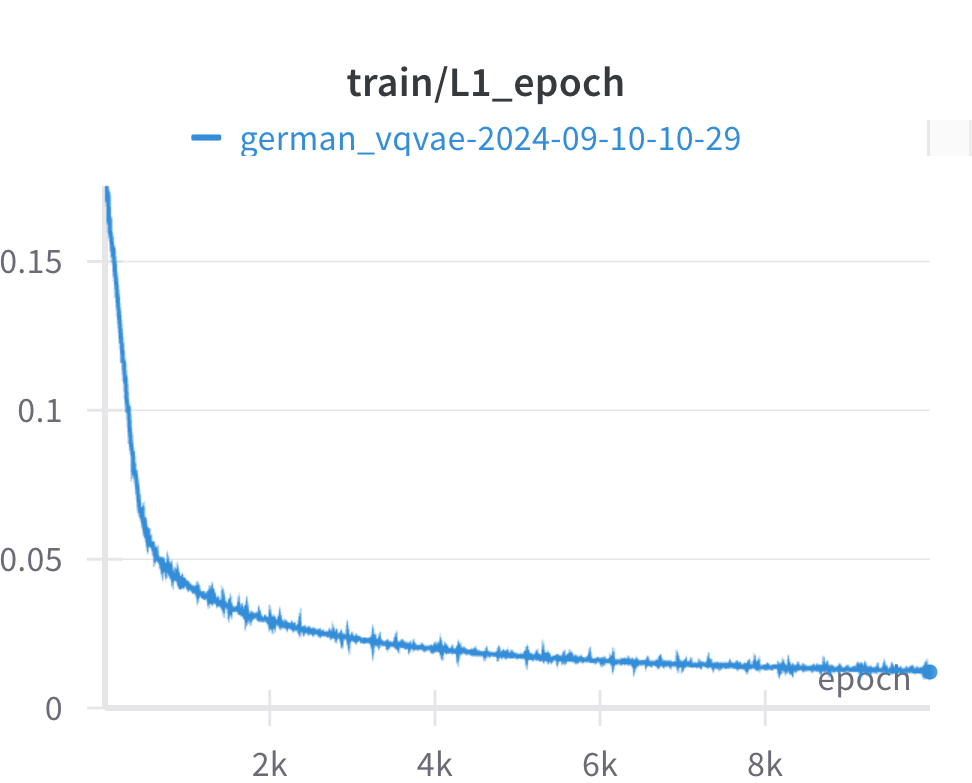
\includegraphics[width=\linewidth]{detailed_engineering/German VQVAE/charts/train_l1.png}
\caption{}
\endminipage\hfill
\minipage{0.49\textwidth}
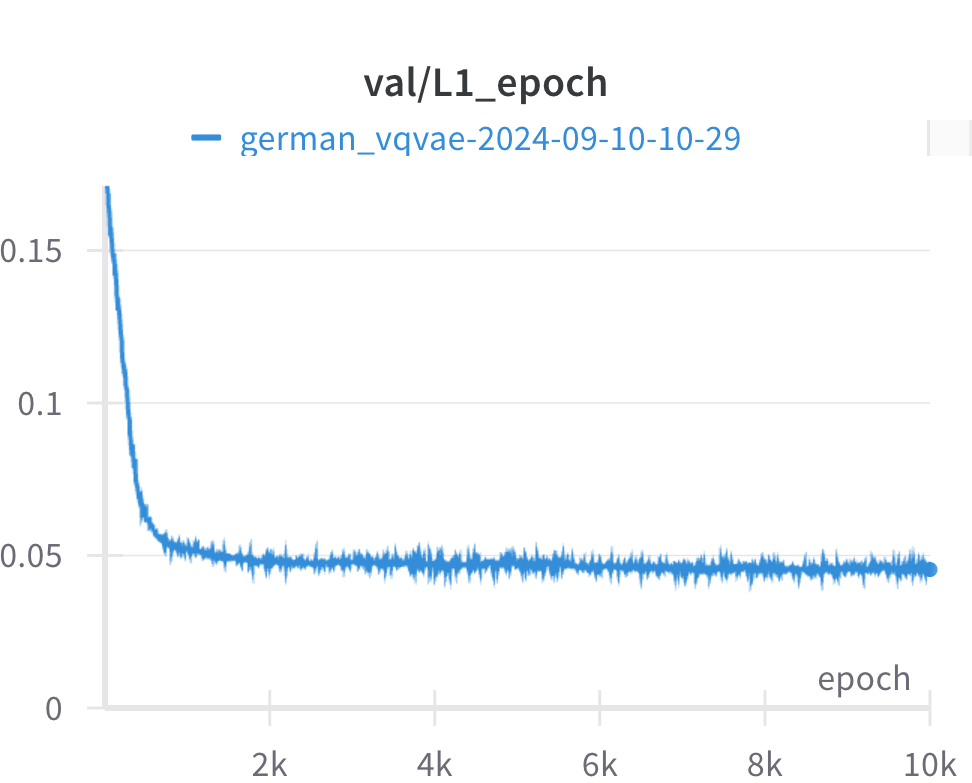
\includegraphics[width=\linewidth]{detailed_engineering/German VQVAE/charts/val_l1.png}
\caption{}
\endminipage
\end{figure}

\begin{figure}[H]
\minipage{0.49\textwidth}
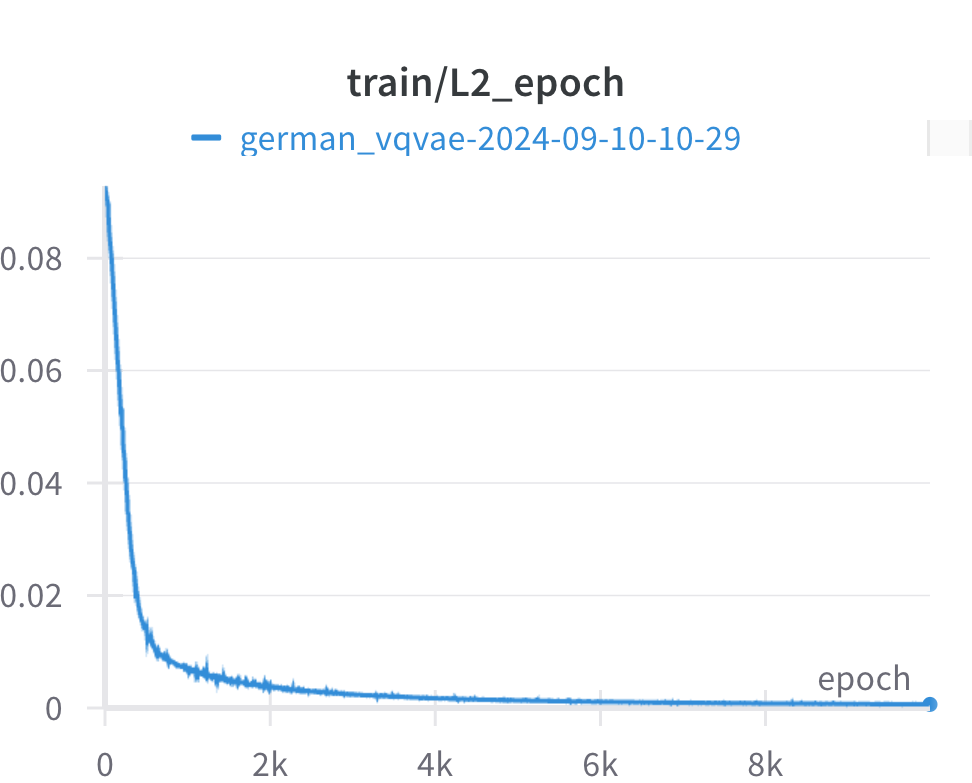
\includegraphics[width=\linewidth]{detailed_engineering/German VQVAE/charts/train_l2.png}
\caption{}
\endminipage\hfill
\minipage{0.49\textwidth}
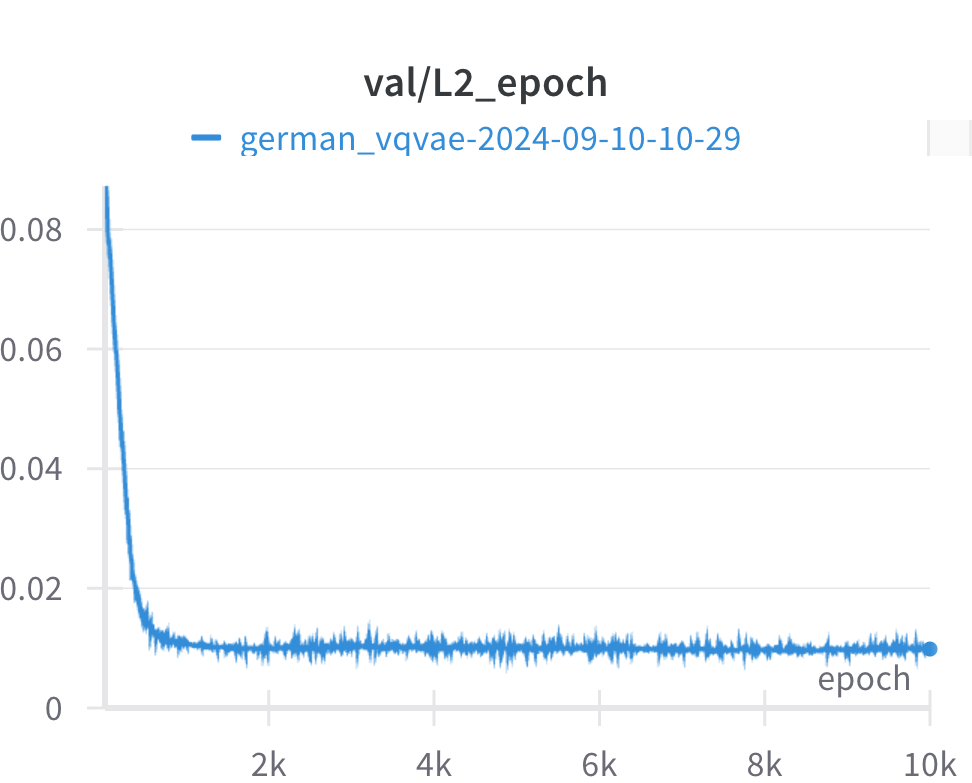
\includegraphics[width=\linewidth]{detailed_engineering/German VQVAE/charts/val_l2.png}
\caption{}
\endminipage
\end{figure}

\begin{figure}[H]
\minipage{0.49\textwidth}
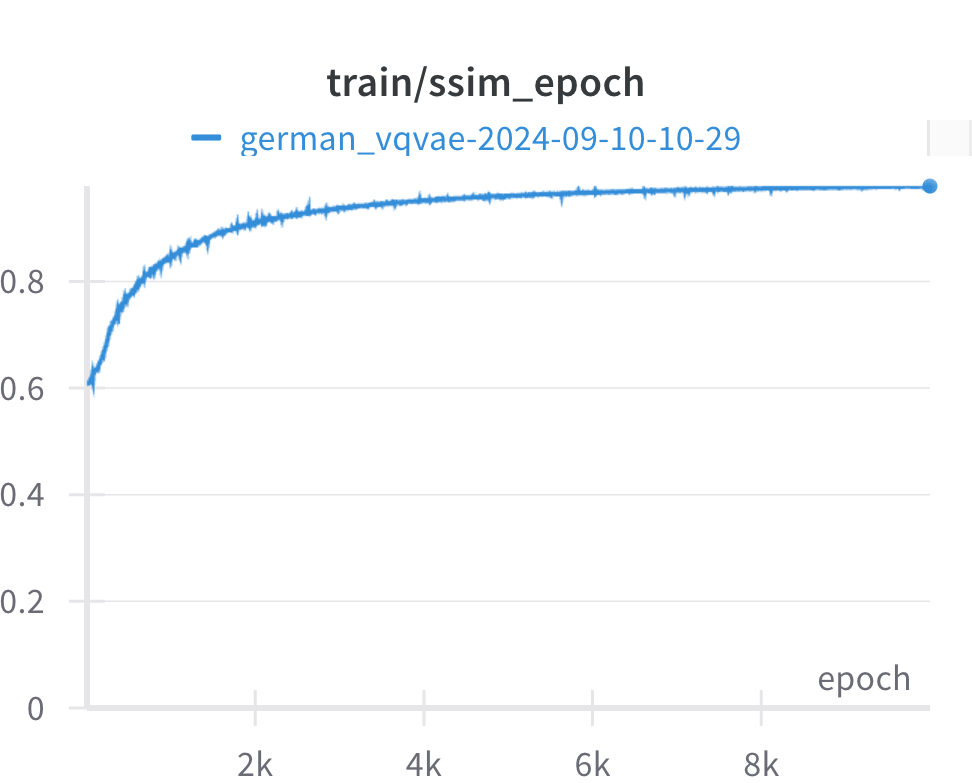
\includegraphics[width=\linewidth]{detailed_engineering/German VQVAE/charts/train_ssim.png}
\caption{}
\endminipage\hfill
\minipage{0.49\textwidth}
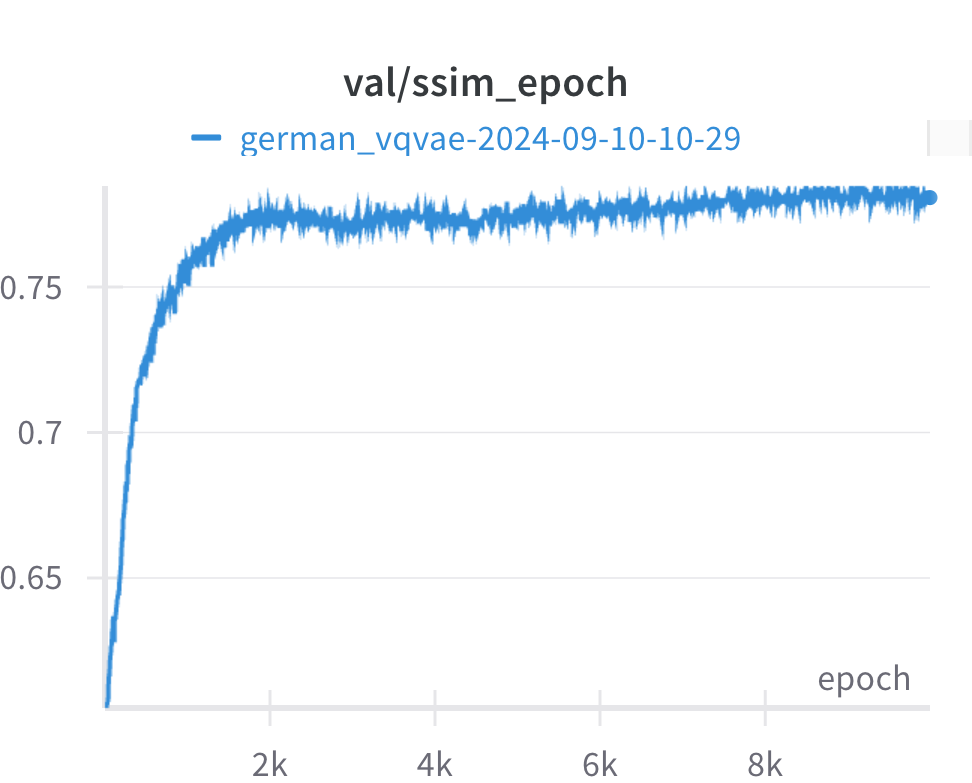
\includegraphics[width=\linewidth]{detailed_engineering/German VQVAE/charts/val_ssim.png}
\caption{}
\endminipage
\end{figure}




\paragraph{Results}\mbox{}\\

\begin{figure}[H]
    \centering
    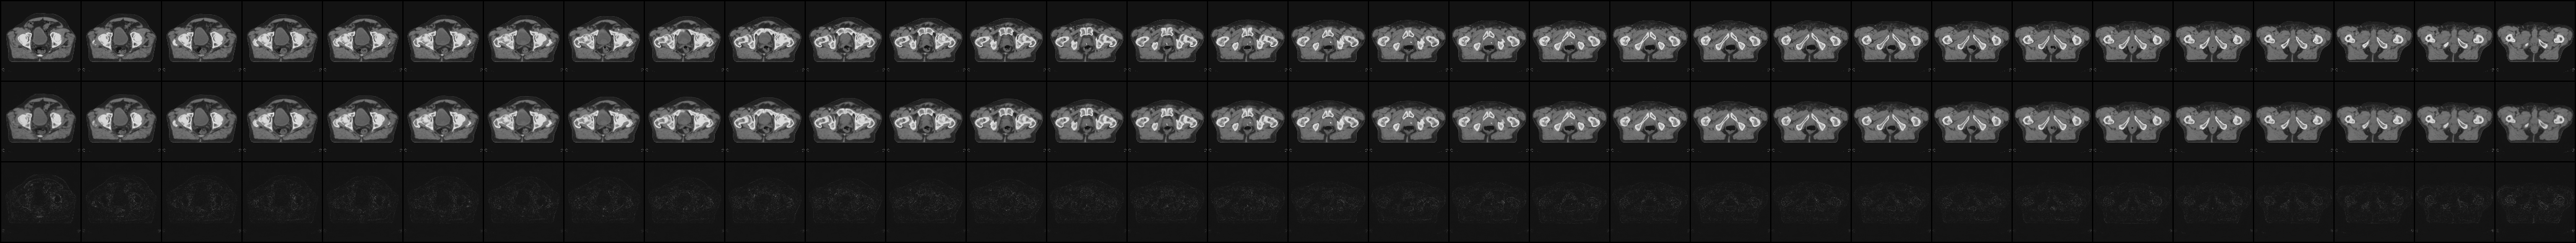
\includegraphics[width=\linewidth]{detailed_engineering/German VQVAE/charts/best_german_vqvae.png}
    \caption{The best quality reconstruction achieved. Epoch 8499, step 10540. Top - input, middle - reconstruction, bottom their difference}
    \label{fig:german_vqvae_best}
\end{figure}


\newpage
\subsubsection{Medical Diffusion: VQGAN + LDM}
\paragraph{Model configuration}

\paragraph{Training}
Objective: Minimize loss function defined as:

\begin{figure}[H]
\centering
\begin{subfigure}[h]{.45\linewidth}
    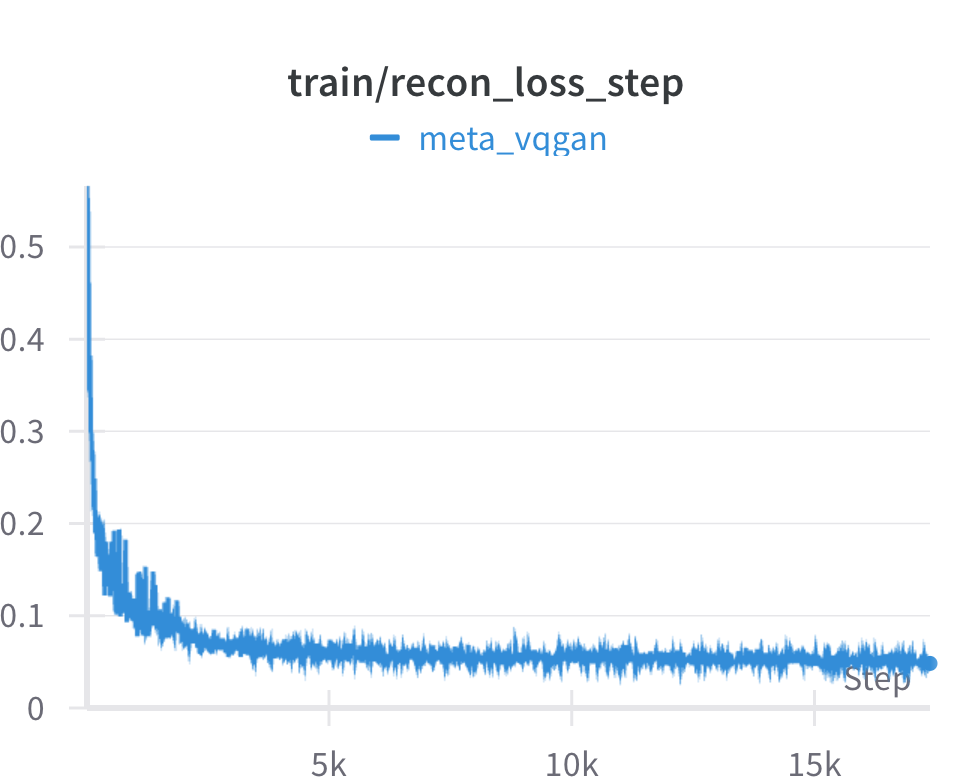
\includegraphics[width=\linewidth]{detailed_engineering/Meta VQGAN/charts/train_recon_loss_step.png}
    \caption{Caption}
    \label{fig:enter-label}
\end{subfigure}
\hfill
\begin{subfigure}[h]{.45\linewidth}
    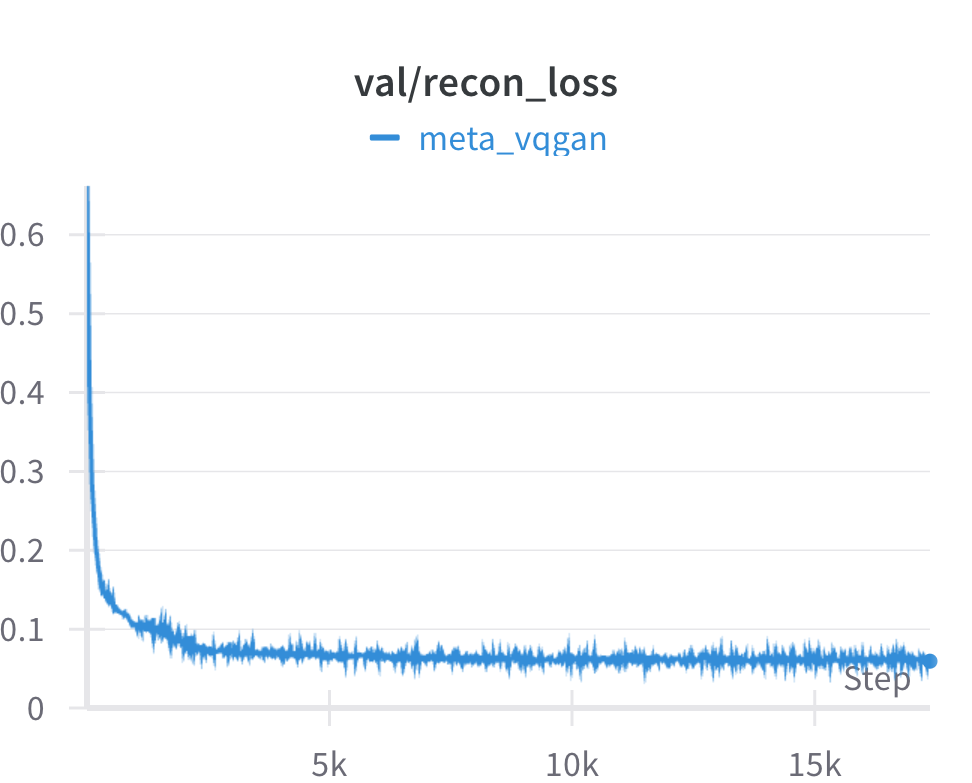
\includegraphics[width=\linewidth]{detailed_engineering/Meta VQGAN/charts/val_recon_loss.png}
    \caption{Caption}
    \label{fig:enter-label}
\end{subfigure}
\hfill
\begin{subfigure}[h]{.45\linewidth}
    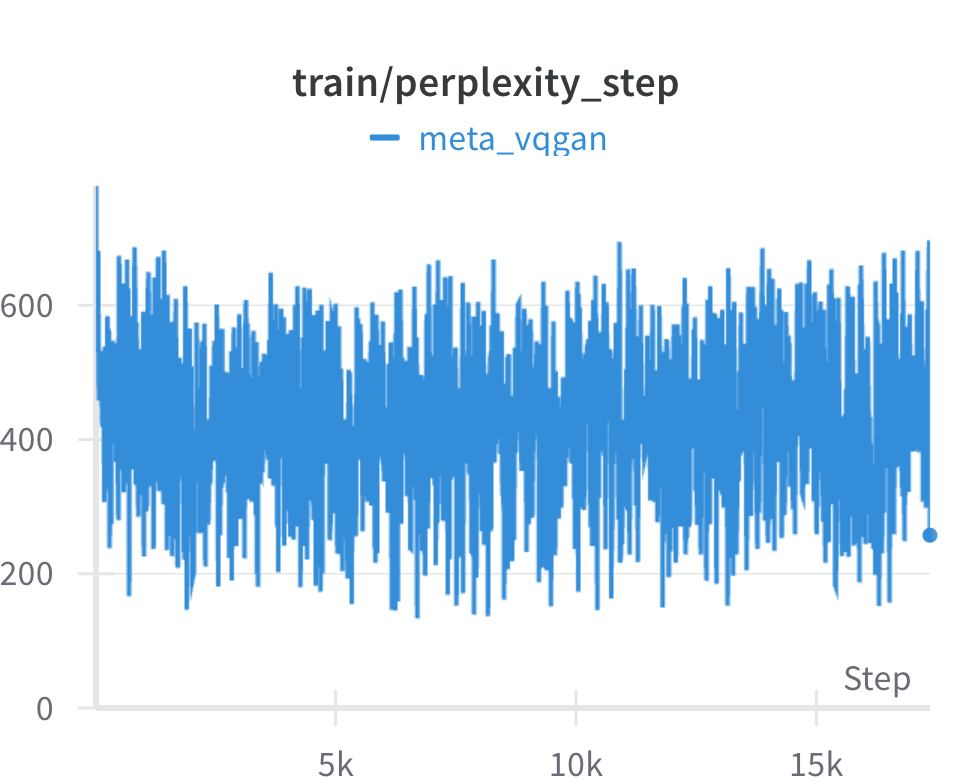
\includegraphics[width=\linewidth]{detailed_engineering/Meta VQGAN/charts/train_perplexity_step.png}
    \caption{Caption}
    \label{fig:enter-label}
\end{subfigure}
\hfill
\begin{subfigure}[h]{.45\linewidth}
    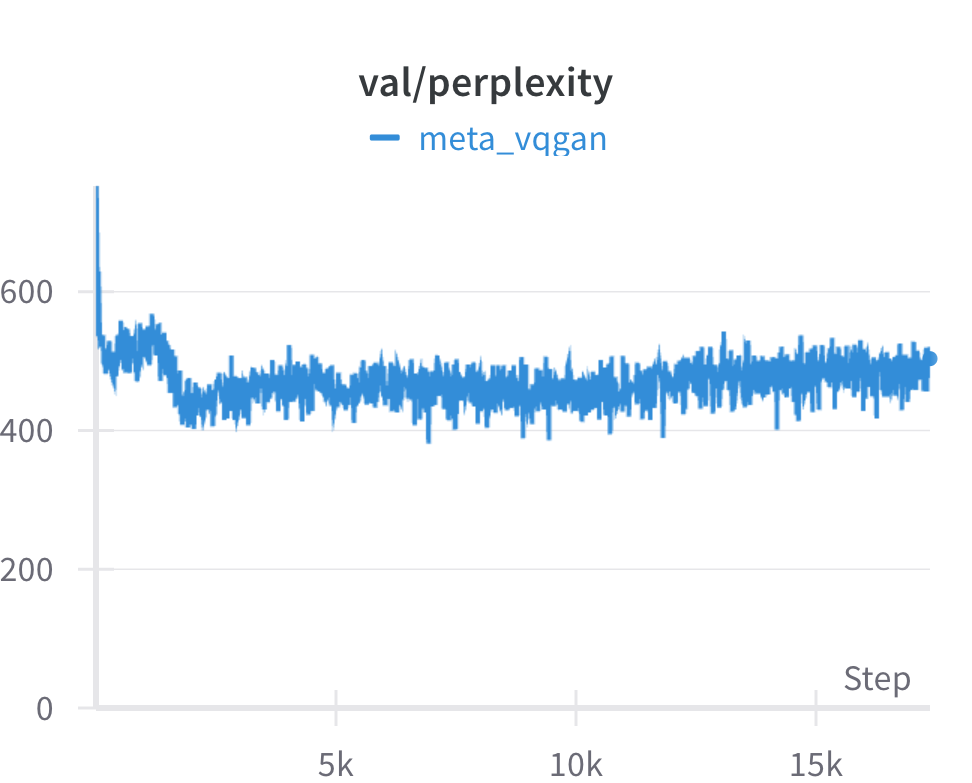
\includegraphics[width=\linewidth]{detailed_engineering/Meta VQGAN/charts/val_perplexity.png}
    \caption{Caption}
    \label{fig:enter-label}
\end{subfigure}
\hfill
\begin{subfigure}[h]{.45\linewidth}
    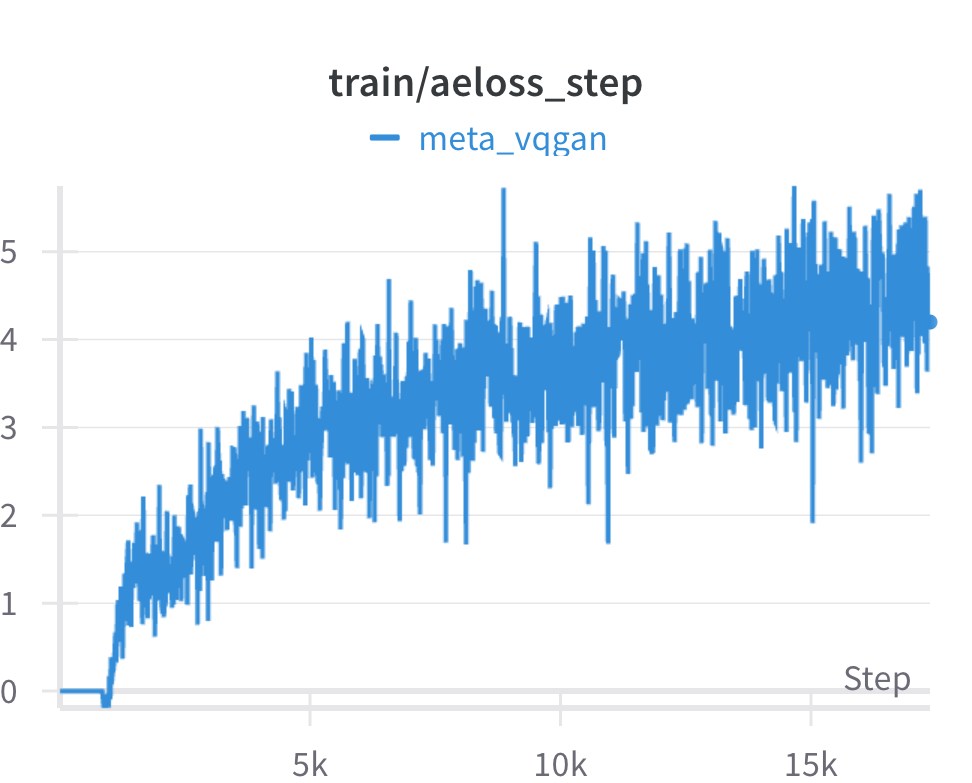
\includegraphics[width=\linewidth]{detailed_engineering/Meta VQGAN/charts/train_aeloss_step.png}
    \caption{Caption}
    \label{fig:enter-label}
\end{subfigure}
\hfill
\begin{subfigure}[h]{.45\linewidth}
    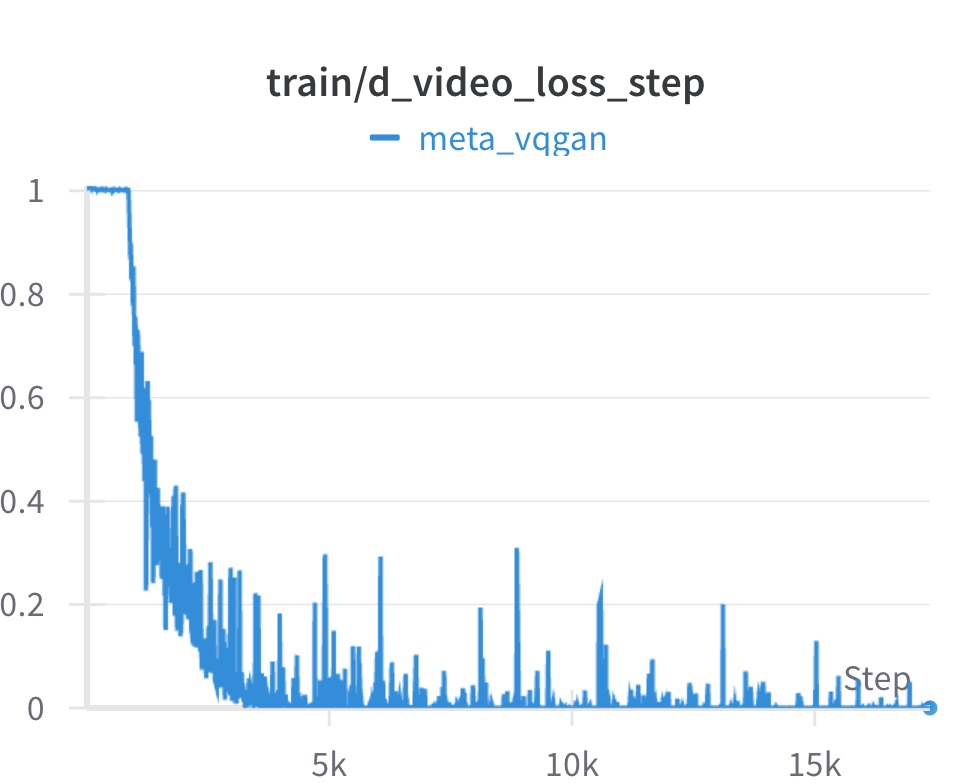
\includegraphics[width=\linewidth]{detailed_engineering/Meta VQGAN/charts/train_d_video_loss_step.png}
    \caption{Caption}
    \label{fig:enter-label}
\end{subfigure}
\hfill
% \begin{subfigure}[h]{.45\linewidth}
%     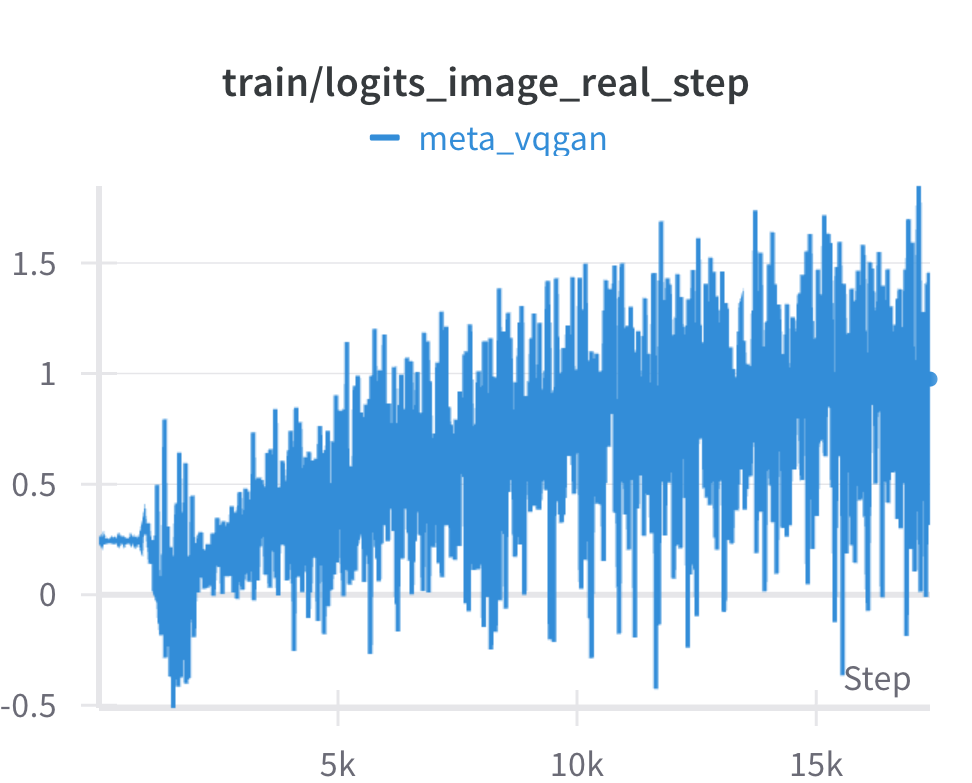
\includegraphics[width=\linewidth]{detailed_engineering/Meta VQGAN/charts/train_logits_image_real_step.png}
%     \caption{Caption}
%     \label{fig:enter-label}
% \end{subfigure}
% \hfill
% \begin{subfigure}[h]{.45\linewidth}
%     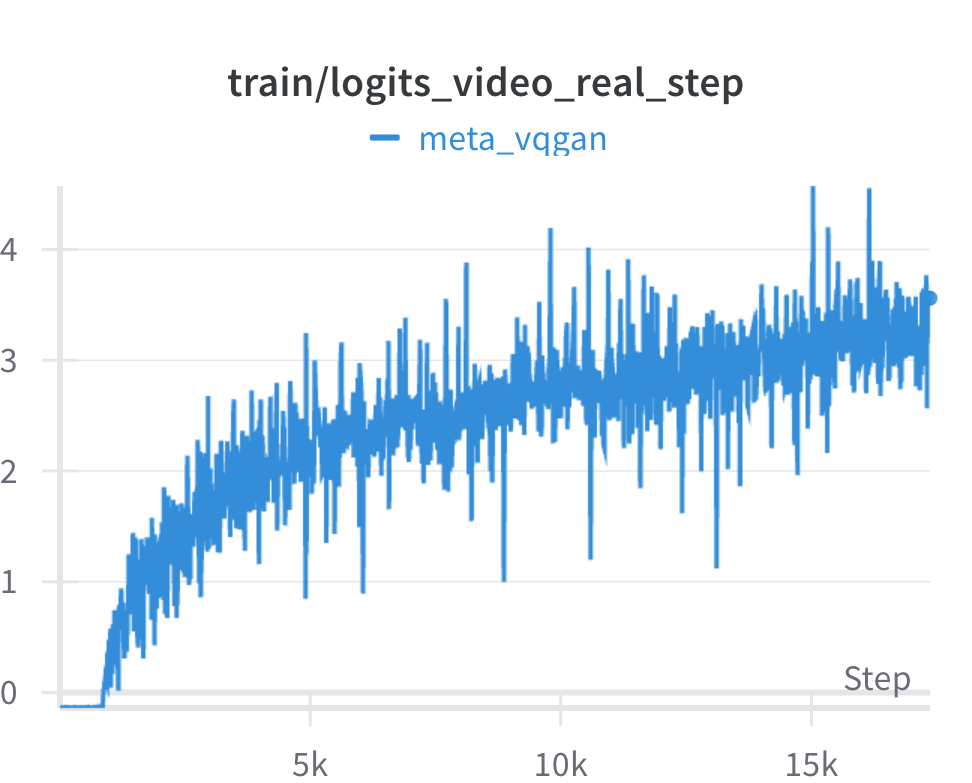
\includegraphics[width=\linewidth]{detailed_engineering/Meta VQGAN/charts/train_logits_video_real_step.png}
%     \caption{Caption}
%     \label{fig:enter-label}
% \end{subfigure}
\hfill
\begin{subfigure}[h]{.45\linewidth}
    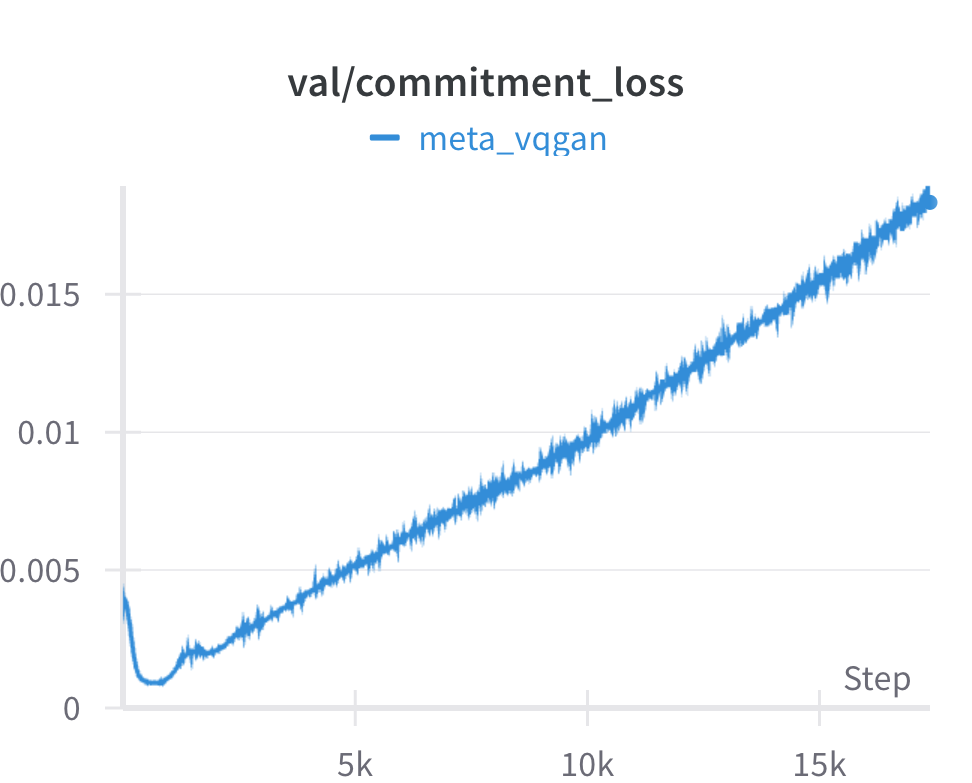
\includegraphics[width=\linewidth]{detailed_engineering/Meta VQGAN/charts/val_commitment_loss.png}
    \caption{Caption}
    \label{fig:enter-label}
\end{subfigure}
\hfill
\begin{subfigure}[h]{.45\linewidth}
    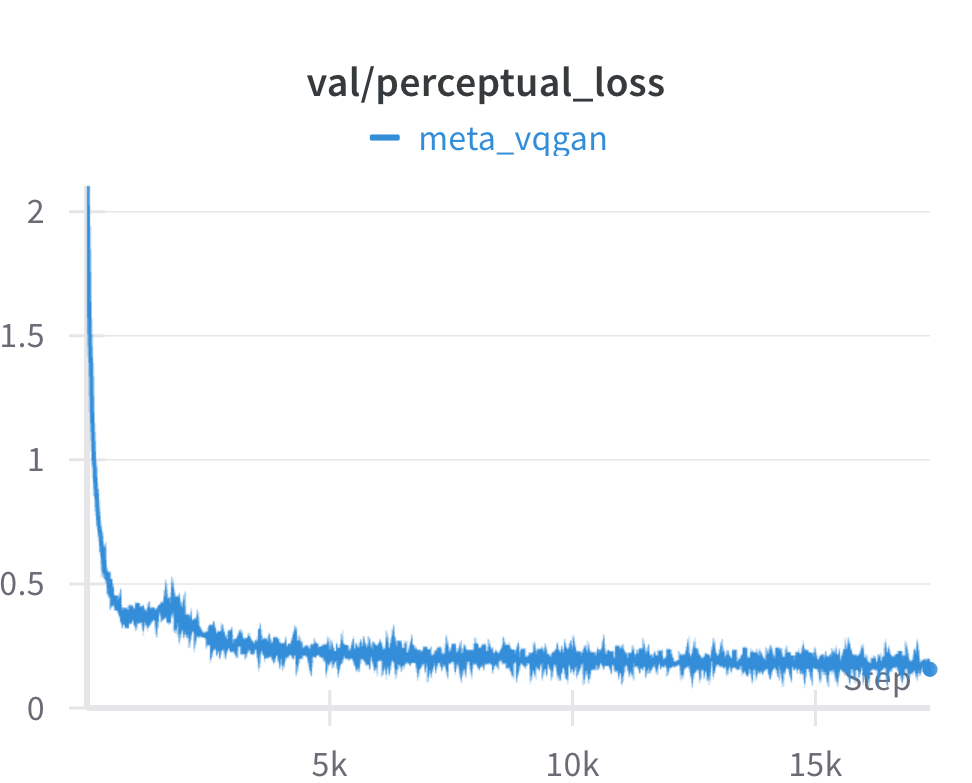
\includegraphics[width=\linewidth]{detailed_engineering/Meta VQGAN/charts/val_perceptual_loss.png}
    \caption{Caption}
    \label{fig:enter-label}
\end{subfigure}
\end{figure}


\paragraph{Results}

\newpage
\paragraph{Medical Diffusion DDPM}
\paragraph{Model configuration}

% \paragraph{Training}
% \begin{figure}[H]
% \centering
% \begin{subfigure}[h]{.45\linewidth}
%     \includegraphics[width=\linewidth]{detailed_engineering/}
%     \caption{Caption}
%     \label{fig:enter-label}
% \end{subfigure}
% \hfill
% \begin{subfigure}[h]{.45\linewidth}
%     \includegraphics[width=\linewidth]{detailed_engineering/Monai Autoencoder/charts/Section-4-Panel-2-bm1y05a9m.png}
%     \caption{Caption}
%     \label{fig:enter-label}
% \end{subfigure}
% \hfill
% \begin{subfigure}[h]{.45\linewidth}
%     \includegraphics[width=\linewidth]{detailed_engineering/Monai Autoencoder/charts/Section-4-Panel-3-dkwhik6ki.png}
%     \caption{Caption}
%     \label{fig:enter-label}
% \end{subfigure}
% \hfill
% \begin{subfigure}[h]{.45\linewidth}
%     \includegraphics[width=\linewidth]{detailed_engineering/Monai Autoencoder/charts/Section-4-Panel-4-d216pe2qa.png}
%     \caption{Caption}
%     \label{fig:enter-label}
% \end{subfigure}
% \hfill
% \begin{subfigure}[h]{.45\linewidth}
%     \includegraphics[width=\linewidth]{detailed_engineering/Monai Autoencoder/charts/Section-4-Panel-5-z2xepgyu7.png}
%     \caption{Caption}
%     \label{fig:enter-label}
% \end{subfigure}
% \end{figure}


\paragraph{Results}


\subsection{Evaluation}

In the table below, autoencoders with their reconstruction quality metrics are presented. 
In addition, the $LDM$ generation quality was measured in the same way. The generative model is treated as if it were a reconstructor, the same as an autoencoder.

In order to profesionally evaluate quality of the generated dataset, the FID score should be calculated. Since the FID score is related to images, not scans or videos, each layer has been analyzed separately. 
A synthetic data set of 28 images (length of the original data set) was created. Then each corresponding layer of scans was analyzed by FID. The mean FID score for each layer in the synthethic dataset is equal to 244.65. 

The number is high compared to the ones in the VQGAN paper\cite{esser2021tamingtransformershighresolutionimage}. It could be caused by the fact that LDM may not generate the internals of the body in the correct order, as can be seen in the figure \ref{fig:ldm-success-comparison}. However, it should be acknowledged by a radiology specialist or doctor of medicine.
\begin{table}[h!]
\centering
\begin{tabular}{|c|c|c|c|c|}
\hline
\textbf{Metric} & VAE & VQVAE1 & Medical Diffusion VQVAE & \textbf{LDM} \\
\hline
$\overline{L1}$ & 0.0309 & 0.0212 & 0.0144 & 0.0845 \\
\hline
$\overline{L2}$ & 0.0043 & 0.0023 & 0.0007 & 0.0270 \\
\hline
$\overline{SSIM}$ & 0.8690 & 0.9399 & 0.9795 & 0.5954 \\
\hline
$\overline{LPIPS}$ & 2.2485 & 1.3820 & 0.8898 & 3.3926 \\
\hline
\end{tabular}
\caption{Mean metrics of the model on the whole dataset as inputs and their reconstructions.}
\label{table:metrics}
\end{table}


% \input{monai}

% \newpage
% \section{Technical feasibility}
% \subsection{Strengths}
% \subsection{Weaknesses}
% \subsection{Opportunities}
% \subsection{Threats}

% \newpage
% \section{Economical feasibility}

% \newpage
% \section{Regulations and legal aspect}

\newpage
\section{Summary}
This project assessed the performance of the VAE, VQVAE, and VQGAN models for generating synthetic prostate CT scans. The implementation utilized modern GPUs and multi-GPU training methods. Tensorboard and WanDB were employed to monitor the AI model training. The execution environment was set up with cutting-edge technologies, Devbox and Rye, to ease future work. Furthermore, the project was initiated with a template that is widely adopted as a standard in the Data Science community.

 The results obtained allowed us to compare them and select the best one. This turned out to be the Medical Diffusion model (VQGAN + U-Net3D LDM) model\cite{khader2023medicaldiffusiondenoisingdiffusion}, which produces visually coherent and good quality prostate scans from Gaussian noise.  

\paragraph{The next steps}\mbox{}\\
\indent The next action that can be taken involves improving both the resolution and the dimensions of the scans. The enhancement in quality can be done by fine-tuning the parameters of the VQGAN model, with particular attention to the Autoencoder segment. A plausible method to accomplish this is to alter the codebook size and correspondingly adjust the scan size within the latent space.

Higher-quality images could possibly be also obtained using a transformer architecture that learns the connections between the encoding vectors and then generates images by the next embeeding prediction\cite{esser2021tamingtransformershighresolutionimage}\cite{khader_transformers_2023}. An another approach could be replacement of the denoising U-Net with the Diffusion Transformer\cite{peebles2023scalablediffusionmodelstransformers} or the Multi-Modal Diffusion Transformer\cite{esser2024scaling}, which is used in Stable Diffusion 3\cite{esser2024scaling}.  

Due to the fact that scans exceeding dimensions of 128x128 could not be handled by the graphics card, this particular size was employed for the majority of the models. In circumstances where it is necessary to produce larger scans, one can utilize the Fully Sharded Data Parallel technique or use a high-resolution technique mentioned in the VQGAN paper\cite{esser2021tamingtransformershighresolutionimage}. 

Nevertheless, in situations where the WFiIS "dose3d" computer operates at an insufficient speed or out-of-memory issues occur again, it is recommended to switch to a different computational system, such as an Athena supercomputer at Cyfronet AGH.



\newpage
\section{Annex}
% Opisać cel wykonania generacji

% Motywacja i cel = 2 strony
% \documentclass[a4paper,12pt]{article}

%te paczki zapewniają język polski
\usepackage[utf8]{inputenc}
\usepackage[english]{babel}
%\usepackage[T1]{fontenc}
% \usepackage{polski}

\usepackage{indentfirst} %pierwsza linia jest z wcięciem (w ang nie, stąd potrzeba tej paczki)
\usepackage{perpage} %the perpage package
\MakePerPage{footnote} %restartuje numerowanie footnotes

%potrzebna do wszelkich matematycznych rzeczy (macierze, specjalne znaki zbiorów, itp.)
\usepackage{amsmath}
\usepackage[normalem]{ulem}
\usepackage{amsfonts}
\usepackage{adjustbox}
%\usepackage{framed} %pozwala na ramki

\usepackage{graphicx, animate} %grafika i obrazy
\usepackage{wrapfig} %do umiejscawiania grafiki
\usepackage{color} %kolorki
\usepackage{geometry} %jakies dodatkowe ustawienia
\usepackage{array} %pionowe centrowanie tekstu w tabelach -> P{}
\usepackage{tabularx} %dostowany tabular, ktory automatycznie łamie zbyt długie komórki
\usepackage{float}
\usepackage{xurl} %dlugie linki
\usepackage[sorting=none, maxnames=4]{biblatex} %bibliografia
\addbibresource{bibliography.bib}
\usepackage{subcaption} %podpisy podwykresow
\usepackage{titlesec}
%definicja wymiarów stron
\geometry{hmargin={2cm, 2cm}, height=10.0in}

\usepackage{hyperref} %spis treści
\newcolumntype{P}[1]{>{\centering\arraybackslash}p{#1}}
\newcommand{\mmathbf}[1]{$\mathbf{#1}$}
\renewcommand{\thefootnote}{\fnsymbol{footnote}}

\newenvironment{conditions*}
  {
  \noindent gdzie:
  \par
  \vspace{\abovedisplayskip}\noindent
   \tabularx{\columnwidth}{>{$}l<{$} @{${}-{}$} >{\raggedright\arraybackslash}X}}
  {\endtabularx\par\vspace{\belowdisplayskip}}
  
\usepackage[linesnumbered]{algorithm2e} 
\usepackage{tikz-cd}
\usepackage{tikz}
\usetikzlibrary{positioning, shapes, shapes.geometric, arrows.meta, calc}


% K0D

% \usepackage[skip=1pt]{caption}
% \captionsetup[subfigure]{aboveskip=0pt}
\usepackage{listings ,pmboxdraw}
\lstset{
  basicstyle=\ttfamily,
  columns=fullflexible,
  keepspaces,
  literate=
  {┐}{\textSFiii}1%
  {└}{\textSFii}1%
  {┴}{\textSFvii}1%
  {┬}{\textSFvi}1%
  {├}{\textSFviii}{1}%
  {─}{\textSFx}1%
  {│}{\textSFxi}1%
  {┼}{\textSFv}1,
}

\usepackage{xcolor}
\usepackage{svg}

\definecolor{codegreen}{rgb}{0,0.6,0}
\definecolor{codegray}{rgb}{0.5,0.5,0.5}
\definecolor{codepurple}{rgb}{0.58,0,0.82}
\definecolor{backcolour}{rgb}{0.95,0.95,0.92}

\lstdefinestyle{mystyle}{
    backgroundcolor=\color{backcolour},   
    commentstyle=\color{codegreen},
    keywordstyle=\color{magenta},
    numberstyle=\tiny\color{codegray},
    stringstyle=\color{codepurple},
    basicstyle=\ttfamily\footnotesize,
    breakatwhitespace=false,         
    breaklines=true,                 
    captionpos=b,                    
    keepspaces=true,                 
    numbers=left,                    
    numbersep=5pt,                  
    showspaces=false,                
    showstringspaces=false,
    showtabs=false,                  
    tabsize=2
}

\lstset{style=mystyle}

% my parg
\newcommand{\myparagraph}[1]{\paragraph{#1}\mbox{}\\}

\usepackage{amsmath, amssymb, latexsym}
\usepackage{sidecap}
 
\usepackage{tikz}
\usetikzlibrary{decorations.pathreplacing}
 \usepackage[mode=build]{standalone}
\usepackage{import}


\let\oldref\ref
\renewcommand{\ref}[1]{(\oldref{#1})} % () przy referencjach

\newcommand{\myref}[1]{(\ref{#1})} % () przy referencjach

\makeatletter
\newcounter{subsubparagraph}[subparagraph]
\renewcommand\thesubsubparagraph{%
  \thesubparagraph.\@arabic\c@subsubparagraph}
\newcommand\subsubparagraph{%
  \@startsection{subsubparagraph}    % counter
    {6}                              % level
    {\parindent}                     % indent
    {3.25ex \@plus 1ex \@minus .2ex} % beforeskip
    {-1em}                           % afterskip
    {\normalfont\normalsize\bfseries}}
\newcommand\l@subsubparagraph{\@dottedtocline{6}{10em}{5em}}
\newcommand{\subsubparagraphmark}[1]{}
\makeatother
\begin{document}
% \documentclass[twoside,11pt,a4paper]{article}[standalone]
% /newcommand{\newind}[]{\newline \indent}


\subsection{Motivation}

\end{document}
\newpage
% ~\newpage
% Opis modelu 
% W jaki sposób i co badamy
% 7 stron
% \import{./}{./implementation}
\setlength\intextsep{0.3cm}

% \newpage
% \section{Results analysis}
% Jakie uzyskano wyniki

% z innych metod, szumów, artefaktów ... etc. 
% 10 stron ok.
% 2 strony
\newpage
% \import{./}{summary.tex}
\newpage
% \section{Dodatek}
% \input{Appendix}
\newpage
\printbibliography[heading=bibintoc,title=Bibliography]
\end{document}